\documentclass[
	main=english,
	ruledheaders=section,%Ebene bis zu der die Überschriften mit Linien abgetrennt werden
	class=book,% Basisdokumentenklasse
	thesis={type=Master Thesis},% Dokumententyp Thesis
	accentcolor=9c,% Auswahl der Akzentfarbe
	custommargins=false, %=true Ränder werden mithilfe von typearea automatisch berechnet (für jede Schriftgröße anders oder so)
	marginpar=false,% Kopfzeile und Fußzeile erstrecken sich nicht über die Randnotizspalte
	BCOR=5mm,%Bindekorrektur
	DIV=10, %gegen Whitespace
	twoside,
	parskip=half-,%Absatzkennzeichnung durch Abstand
	fontsize=11pt,%Basisschriftgröße laut Corporate Design ist mit 9pt häufig zu klein
	%	logofile=example-image, %Falls die Logo Dateien nicht vorliegen
]{tudapub}
% Englische Sprache 
\usepackage[english]{babel}
% Pakete mit Mathesymbolen und zur Beseitigung von Schwächen der Mathe-Umgebung
\usepackage{latexsym,exscale,stmaryrd,amsmath}
% Farbe
\usepackage{color}

%Bibliography and citation
\usepackage[numbers,sort&compress,square]{natbib}
\bibliographystyle{BibtexStyle}
%\bibliographystyle{alpha}

\usepackage{url}

% Für Einheiten
\usepackage[per-mode=symbol, separate-uncertainty=true]{siunitx}
\sisetup{output-decimal-marker={.},list-final-separator={\text{ and }},list-pair-separator={\text{ and }},list-separator={, },list-units=single}
\sisetup{range-phrase={\text{ to }},range-units=brackets, list-units=brackets}
\sisetup{print-zero-exponent=false, print-unity-mantissa=false}
\sisetup{detect-all}
%\sisetup{scientific-notation = engineering}


% Für Captions / Bildunterschriften - keine Einrückung in der zweiten Zeile mehr
\setcapindent{0pt}

%flush figures
\usepackage{placeins}
\usepackage{float}

% Zur Graphikausgabe
%Beipiel: 
%\includegraphics[width=\textwidth]{grafik.png}

% Text umfließt Graphiken und Tabellen
% Beispiel:
% \begin{wrapfigure}[Zeilenanzahl]{"l" oder "r"}{breite}
%   \centering
%   \includegraphics[width=...]{grafik}
%   \caption{Beschriftung} 
%   \label{fig:grafik}
% \end{wrapfigure}
\usepackage{wrapfig}




%---------------------------------------------------------------------
% stuff I added myself
% \usepackage{cite} % so that multiple ref in a cite works
\usepackage{float}
\usepackage{graphicx}
\usepackage{caption}
\usepackage{subcaption}
\usepackage[export]{adjustbox}
\usepackage[font={small}]{caption}
\usepackage{hyperref}
\usepackage{gensymb}
\usepackage{boldline}
\usepackage[titletoc]{appendix}
\usepackage{upgreek}

\usepackage[nottoc]{tocbibind} %Includes "References" in the table of contents

% and some commands I added
\newcommand{\dofigure}[4]{
	\begin{figure}
		\centering
		\includegraphics[width = #1\textwidth]{Diagrams/#2}
		\caption{#3}
		\label{#4}
	\end{figure}
}

\newcommand{\angstrom}{\textup{\AA}}
\newcommand{\eV}[1]{
	\SI{#1}{\electronvolt}
}



%%%%%%%%%%%%%%%%%%%
%Paketvorschläge Tabellen
%%%%%%%%%%%%%%%%%%%
%\usepackage{array}     % Basispaket für Tabellenkonfiguration, wird von den 
%%folgenden automatisch geladen
\usepackage{tabularx}   % Tabellen, die sich automatisch der Breite anpassen
%\usepackage{longtable} % Mehrseitige Tabellen
%\usepackage{xltabular} % Mehrseitige Tabellen mit anpassbarer Breite
\usepackage{booktabs}   % Verbesserte Möglichkeiten für Tabellenlayout über 
%horizontale Linien

%%%%%%%%%%%%%%%%%%%
%Paketvorschläge Mathematik
%%%%%%%%%%%%%%%%%%%
\usepackage{mathtools} % erweiterte Fassung von amsmath
\usepackage{amssymb}   % erweiterter Zeichensatz
\usepackage{makecell}
\usepackage{stackengine}\setstackEOL{\cr} %EOL is abbreviation for "end of line."

%Formatierungen für Beispiele in diesem Dokument. Im Allgemeinen nicht 
%notwendig!
\let\file\texttt
\let\code\texttt
\let\tbs\textbackslash
\let\pck\textsf
\let\cls\textsf

\usepackage{pifont}% Zapf-Dingbats Symbole
\newcommand*{\FeatureTrue}{\ding{52}}
\newcommand*{\FeatureFalse}{\ding{56}}

\begin{document}
	
	\Metadata{
		title=Soft X-Ray Spectrometers for Absorption Spectroscopy of Aluminum in Laser Driven Backlighter Experiments,
		author=Carlos Butler
	}
	
	\title{Soft X-Ray Spectrometers for Absorption Spectroscopy of Aluminum in Laser Driven Backlighter Experiments}
	\subtitle{Spektrometer für weiche 
	Röntgenstrahlung aus 
	laser-getriebenen Quellen zur Absorptionsspektroskopie von Aluminium}
	\author[C. Butler]{Carlos Esteban Butler}%optionales Argument ist die Signatur,
	\birthplace{Florida, USA}%Geburtsort, bei Dissertationen zwingend notwendig
	\reviewer{Prof. Dr. Vincent 
	Bagnoud \and Philipp Hesselbach, M.Sc.}%Gutachter
	\titlegraphic{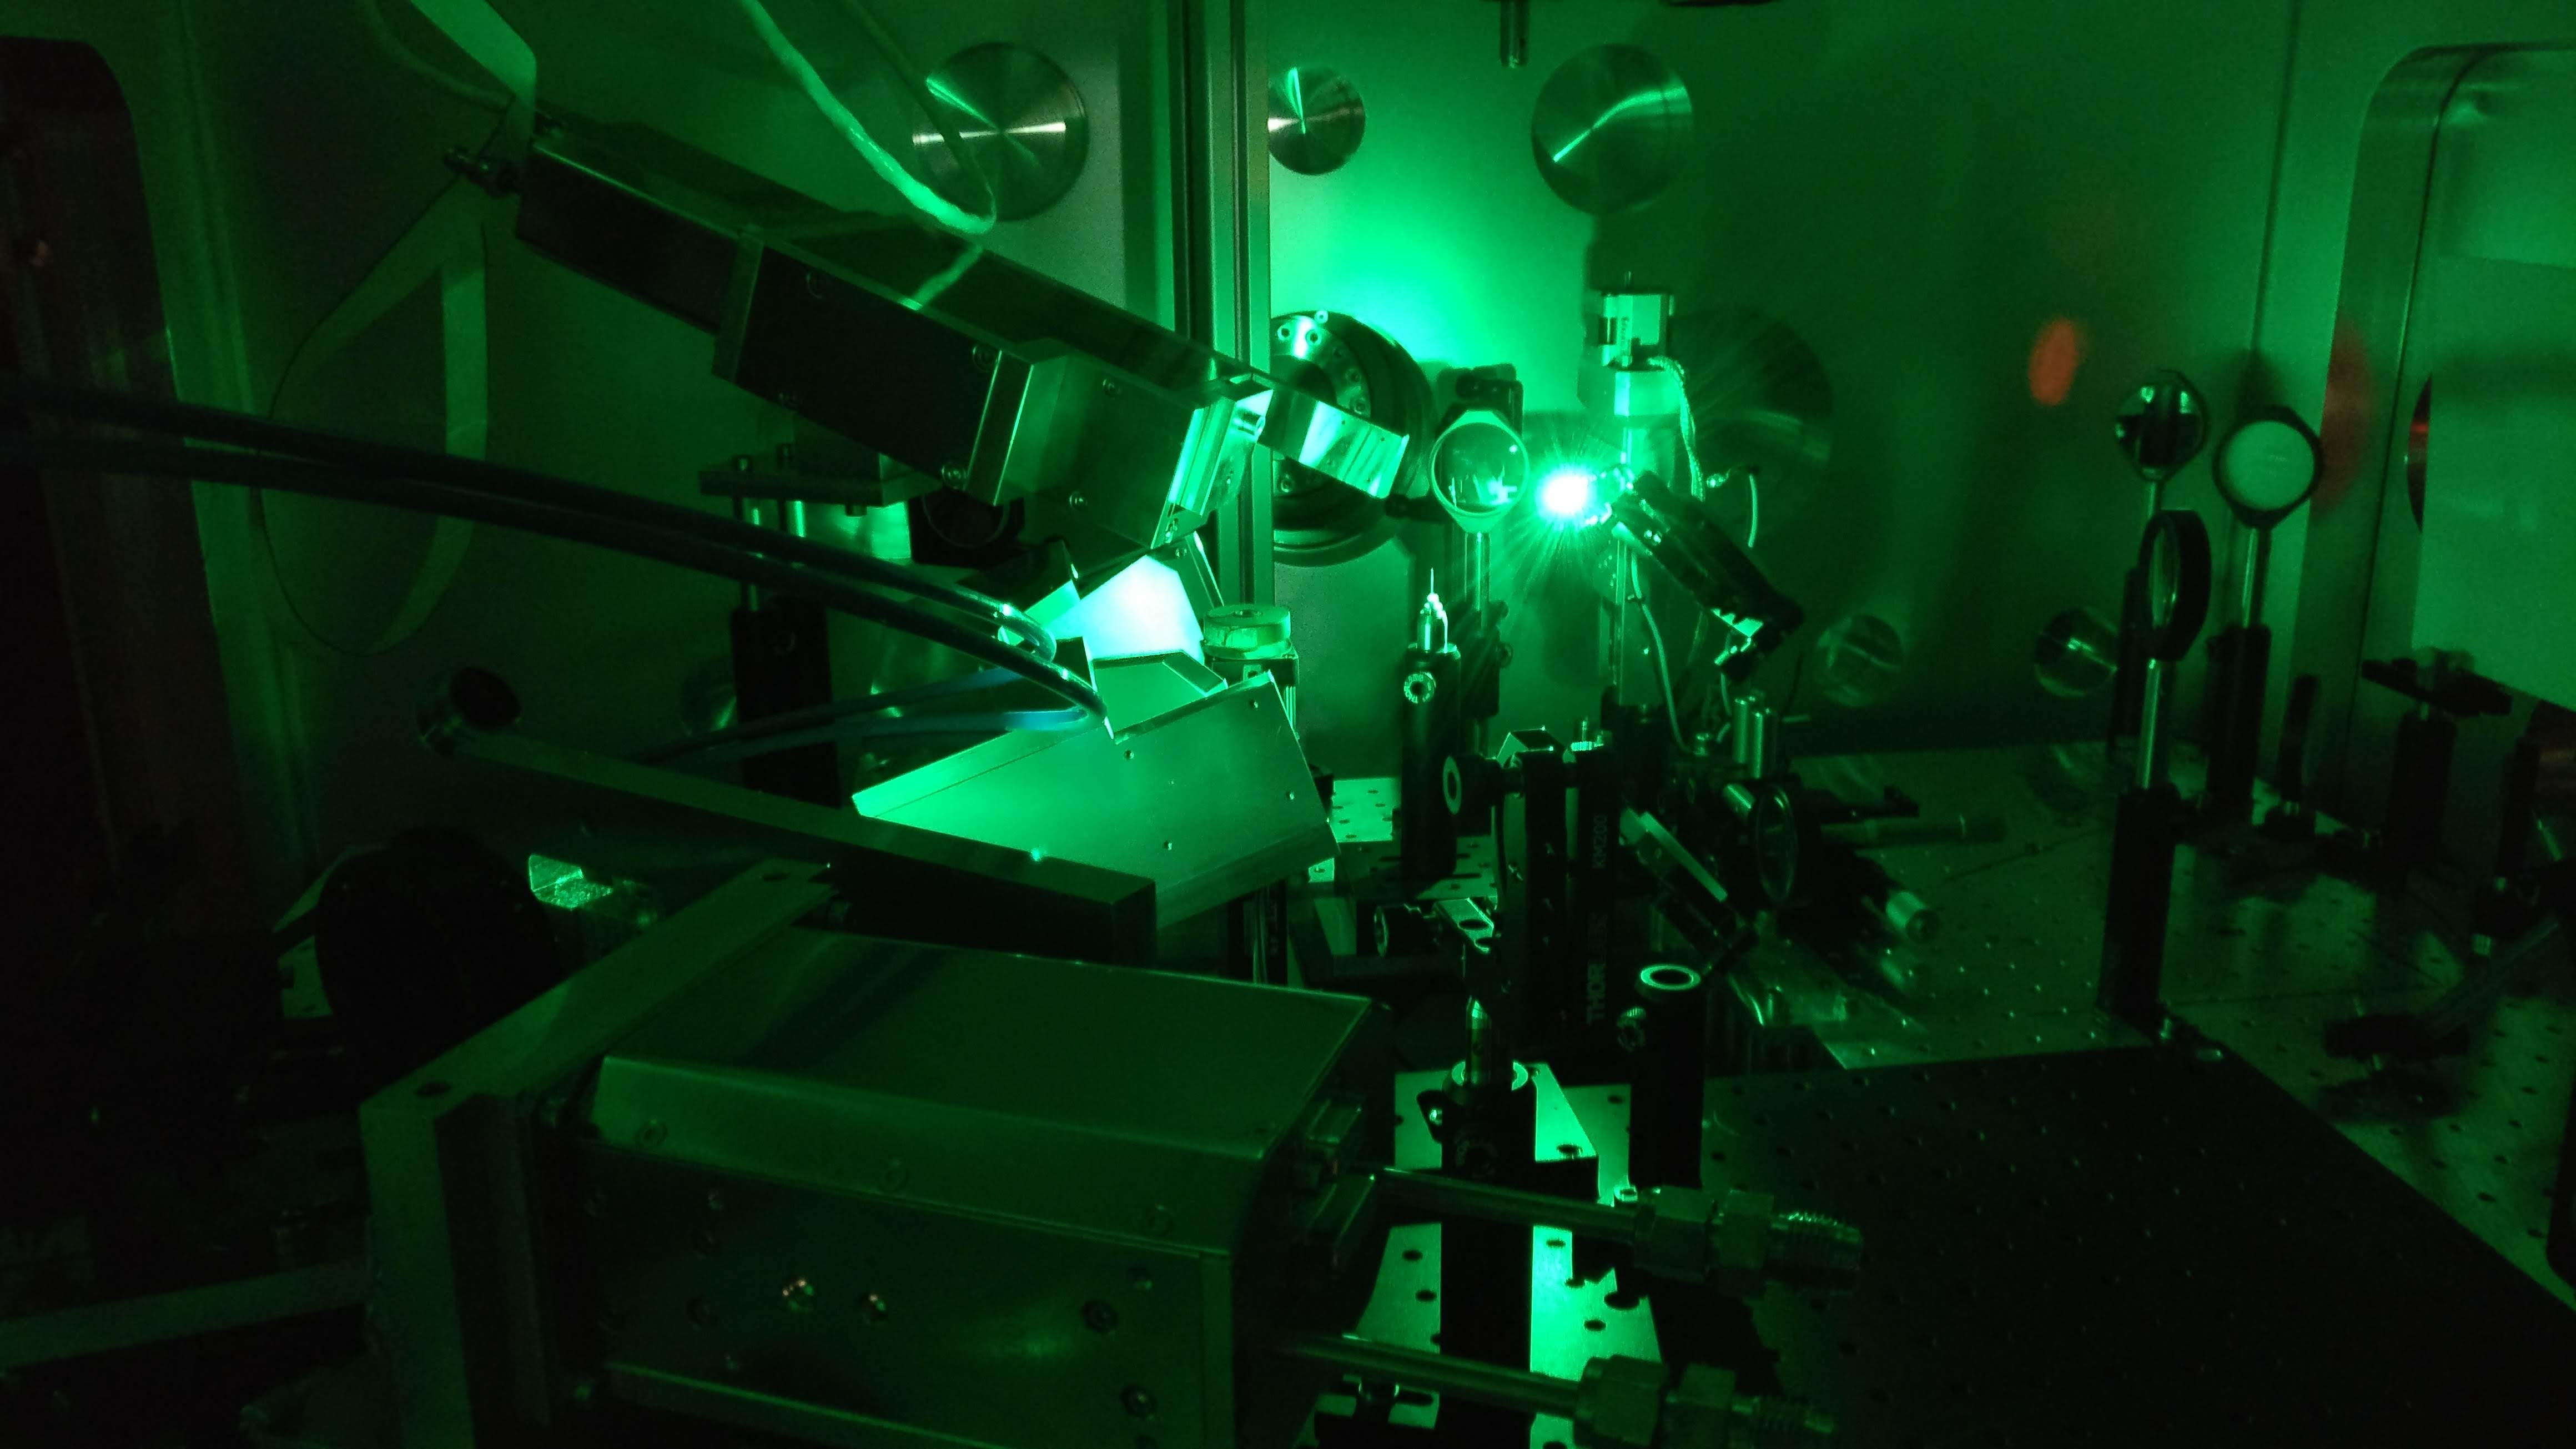
\includegraphics[width=\width]{Diagrams/Title.jpg}}
	
	%Diese Felder werden untereinander auf der Titelseite platziert.
	%\department ist eine notwendige Angabe, siehe auch dem Abschnitt 
	%`Abweichung von den Vorgaben für die Titelseite'
	\department{phys} % Das Kürzel wird automatisch ersetzt und als Studienfach 
	%gewählt, siehe Liste der Kürzel im Dokument.
	\institute{Institute of Nuclear Physics}
	\group{Working Group Bagnoud}
	
	\date{January 16, 2024}
	\examdate{January 16, 2024}
	\tuprints{license=This document is published under the license CC BY-NC 4.0 International \newline\url{creativecommons.org/licenses/by-nc/4.0/},
	urn=urn:nbn:de:tuda-tuprints-275311,
	printid=id/eprint/27531}

	
	% \dedication{Für alle, die \TeX{} nutzen.}
	
	\maketitle
	
	\affidavit
	\chapter*{Acknowledgments}

This thesis would not have been possible without the help of many people. I'd like to thank the plasma physics/PHELIX group at GSI in general for taking me in and supporting me, and of course for the fun times. In particular I want to thank my supervisor Philipp Hesselbach, M.Sc., who supported me every step of the way and offered invaluable advice, and Dr. Paul Neumayer, who gave continued support throughout the thesis, as well as Prof. Dr. Vincent Bagnoud for giving me the opportunity and accommodating my ever-changing plans. The spectrometer designs benefited from the helpful input of Dr. Artem Martynenko, who also gave me great advice and help with the analysis of spectrometer data. The always stressful beamtime was successful (and often fun) thanks to the awesome experiment team of Philipp, Paul, Dr. Zsuzsanna Major, Dr. Bernhard Zielbauer, and Alice Renaux. I'd also like the thank my office roommates René Kalla, Sarah Grimm, Alice, Pierre Lebegue, and Jannis Lutz for the great conversations and dumb jokes. I hope to see all of you again and have you try more of my desserts.

I wouldn't have reached this point in my studies without the help of my family, especially my mom, dad, and siblings, who supported my decisions and were always there for me, during my studies and well before that. A very special shout out goes to my (newly-minted) wife Yan Yi. I don't know what I would do without you.


	
	\tableofcontents
	
	\chapter{Introduction}

The experimental study of warm dense matter (WDM) has 
been gaining steam in the last few decades thanks to 
developments in laser and accelerator 
facilities, allowing researchers to better probe 
these elusive states of matter \citep{riley2021warm, 
falk2018experimental, graziani2014frontiers}. WDM, 
though not precisely defined, is generally considered 
to encompass states with pressures above 
\SI{100}{\giga\pascal}, temperatures in the range of 
\SI{1}{\electronvolt} to \SI{100}{\electronvolt}, and 
high densities, lying at or above solid density 
\citep{riley2021warm}. In this regime the plasma 
displays unique properties, including strongly 
coupled, fluid-like ions and fully or partially 
degenerate electrons, which invalidates many standard 
approximations in the current theory 
\citep{falk2018experimental} and makes WDM difficult 
to 
describe. In addition to this theoretical interest, 
WDM is of great importance to 
many fields, ranging from astrophysics, where the 
study of WDM gives insight into the internal 
structure and evolution of many celestial objects 
\citep{koenig2005progress,collins1998measurements, 
tahir2022planetary}, to inertial confinement fusion, 
relevant for the 
understanding of implosions of laser fusion capsules 
\citep{riley2021warm, falk2018experimental}. 
Consequently, many large-scale 
experiments are conducted on WDM 
\citep{bagnoud2010commissioning, 
millot2019nanosecond, altarelli2011european}, which 
all seek to solve the significant experimental 
challenges inherent to WDM, i.e. the generation of 
extreme conditions 
\citep{koenig2005progress,falk2018experimental} and 
the consequently short lifetimes on 
the order of micro- to nanoseconds 
\citep{riley2021warm}. 

The necessity of rapidly depositing large amounts of 
energy with powerful drivers to reach WDM conditions presents a 
considerable experimental challenge. In general, two main requirements play a role in assessing the viability of a WDM driver. One is uniformity of the sample, as strong temperature or density gradients can hinder comparison with theory and therefore make it difficult to assess the WDM properties. This limitation rules out many direct drivers. The other requirement is timescale. The sample should stay within WDM conditions long enough for probes and optimally allow time for equilibration \citep{riley2017generation}. Since static methods, such as diamond anvil 
cells (DAC), where the sample is confined and compressed between diamond anvils \citep{dubrovinsky2000situ}, only reach temperatures and pressures at the low end of the WDM range ($\approx$\SI{100}{\giga\pascal} and $\lessapprox$\SI{1}{\electronvolt}), dynamic methods are often pursued. 

The dynamic WDM generation methods can be loosely placed in two categories: shock/ramp compression and volumetric heating \citep{riley2017generation}. A notable example of the former type is indirectly laser driven shocks. A high-Z cylindrical hohlraum target is irradiated with intense laser pulses resulting in x-ray emission which, in turn, ablate the top layer of a shock target located in the center of the hohlraum, driving a shock which culminates in the center. This method was successfully applied at the National Ignition Facility (NIF) in California to generate WDM of beryllium \citep{doppner2023observing}. A promising application of the latter type, volumetric heating, comes in the form of ultra-short x-ray pulses from x-ray free-electron lasers (XFEL). These intense pseudo-monochromatic x-ray beams are focused to a spot size of a few microns. Upon irradiating a sample target, the photons are mostly absorbed through photo-absorption in a given band or shell of the material, depositing their energy uniformly within femtoseconds and producing a transient WDM state \citep{riley2017generation}, as demonstrated at the Linac Coherent Light Source (LCLS) facility in California \citep{vinko2012creation}. An alternative approach to volumetric heating, and the one relevant to this work, are intense heavy-ion beams, which transfer energy to a sample through coulomb collisions between the ions in the beam and electrons in the target. For this approach the penetration range is on the 
scale of several mm and heating occurs 
isochorically along the whole sample 
\citep{tahir2008studies}. These properties offer significant advantages in that large (mm$^3$) high-Z WDM samples with sufficient lifetimes for equilibration
and high uniformity can be produced \citep{riley2021warm, tahir2022planetary}, opening doors to new 
WDM physics. 

Similarly to the generation of warm dense matter, the diagnostics and characterization of WDM samples require addressing unique obstacles. Due to the short lifetimes of the state, the diagnostic methods must allow for fast data acquisition. Additionally, the high opacity of WDM samples in the 
optical 
range means that most methods of optical probing are excluded, 
unless performing surface or shock-wave measurements 
\citep{riley2021warm, schoenberg2020high, 
falk2018experimental}. X-rays, on the other hand, are 
capable of penetrating these samples thanks to longer 
attenuation lengths, and therefore 
offer effective diagnostic techniques for probing the 
bulk properties of WDM \citep{torchio2016probing, 
bagnoud2010commissioning}. In order to apply these techniques, intense, fast x-ray sources, also referred to as backlighters, are required. Common methods to produce 
x-rays for WDM experiments include synchrotrons 
\citep{torchio2016probing}, x-ray free-electron lasers \citep{lee2003finite}, and 
laser-driven plasmas. Interestingly, in the case of XFEL, the x-ray beam can simultaneously act as the WDM driver and a selective probe, as shown at the LCLS by \textit{Vinko, et al.} \citep{vinko2012creation}. In the frame of this thesis, laser-driven plasma, generated by
irradiating backlighter targets with a
high-intensity pulsed optical laser, acts as a high-brightness fast x-ray source for the diagnostics, which can be 
tuned to desired energy ranges and intensities 
through the choice of backlighter material and laser 
energy \citep{bagnoud2010commissioning}. The 
tunability, high intensity, and small angular 
dependence of the x-ray emission are especially attractive to WDM 
matter research.

Advances in the area of intense x-ray beam generation enable several diagnostic techniques applicable to WDM research, including 
x-ray scattering, radiography, and 
x-ray absorption spectroscopy \citep{riley2021warm, 
falk2018experimental}. The first method involves studying features in spectrally resolved x-ray scattering measurements and comparing the results to theoretical descriptions of the scattering \citep{riley2017generation}. In this way, \textit{Lee et al.} successfully determined the ion temperature and density of laser-driven dense plasma of beryllium \citep{lee2009x}. Another effective diagnostic technique is X-ray Absorption Fine-Structure Spectroscopy (XAFS), an extension of x-ray absorption spectroscopy, which was first demonstrated in the scope of WDM research in 1987 by \textit{Hall et al.} \citep{hall1988experimental} and is the diagnostic of choice in this work. This method extracts bulk properties of a sample by investigating features of an absorption spectrum located around an absorption edge, defined by the binding energy of a shell of electrons. The features form when electrons released through the photoelectric effect quantum mechanically scatter on neighboring atoms in the sample. The back-scattered photoelectron wave-functions overlap with the electron state at the original atom, modulating the absorption coefficient \citep{newville2014fundamentals}. As this modulation behaves differently depending on proximity to the absorption edge, one distinguishes between X-ray Absorption Near Edge Structure (XANES) and Extended X-ray Absorption Fine-structure (EXAFS), i.e. at photon energies from typically $\sim \SI{50}{\electronvolt}$ above the edge \citep{levy2009x, peyrusse2009k}. As a smaller energy range and higher spectral resolution is required for XANES as compared to EXAFS and because each encompass different theoretical descriptions, experiments commonly target one specifically. Because each sub-technique allows for determining different material properties \citep{riley2021warm}, XAFS can cover a wide range of applications, although it is important to note that the method benefits from a smooth backlighter spectrum as well as an uniform sample to resolve the fine-structures \citep{riley2017generation}. Accordingly, the experimental setup must be designed specifically to match the requirements of XAFS.

The general experimental scheme (see fig. \ref{fig: HIHEX scheme}), which will build the context of this work, seeks to leverage three concepts of WDM research in a novel way: intense heavy-ion beams for WDM generation, laser-driven plasma for backlighting, and XAFS for diagnostics. The heavy-ion beam produces large, highly homogeneous WDM samples, while the high intensity and tunability of the laser-driven backlighter allows for a smooth x-ray source spectrum with a significant x-ray flux. Together, these advantages harmonize well with XAFS to create the possibility of highly resolved absorption spectra of uniform WDM samples, with which bulk properties can be extracted with precision, opening the door to further advances in WDM research. 

\begin{figure}[H]
	\centering
	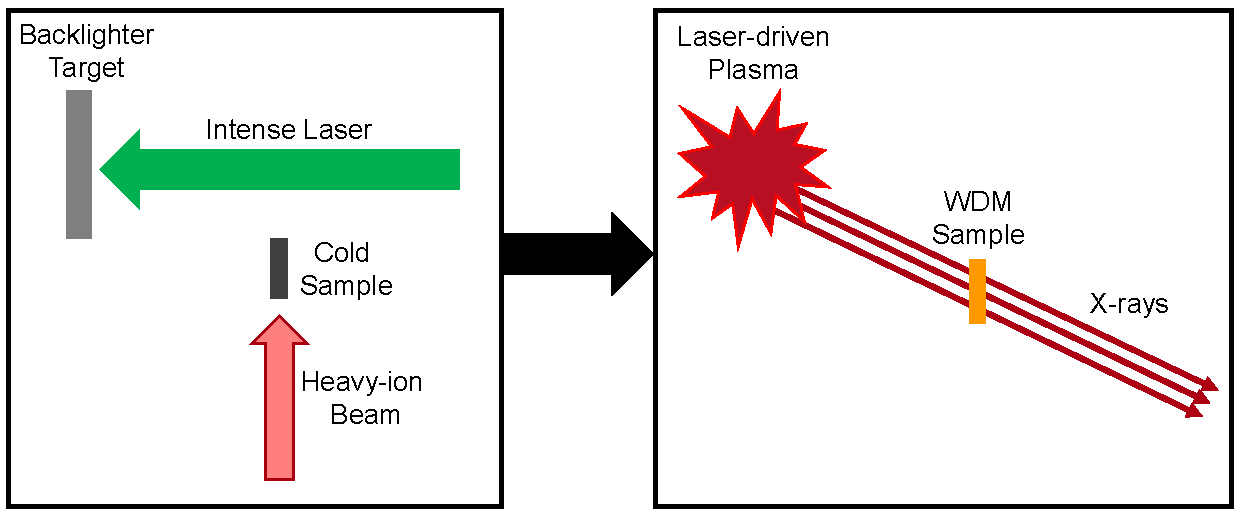
\includegraphics[width=0.85\textwidth]{Diagrams/HIHEX.pdf}
	\caption{Schematic of experiment using heavy ions for WDM generation paired with laser-driven X-ray sources for diagnostics.}
	\label{fig: HIHEX scheme}
\end{figure}

A project utilizing this scheme will be realized at the Facility for Antiproton and 
Ion Research (FAIR), an accelerator facility under 
construction in Darmstadt, Germany 
\cite{schoenberg2020high}, with current research work carried out at a 
neighboring facility, the GSI 
Helmholtz Center for Heavy Ion Research 
\citep{bagnoud2010commissioning}. With the goal of validating the experimental setup and demonstrating a proof of concept, preparatory experiments are conducted at the High energy, High 
Temperature (HHT) experimental station, where high-energy nanosecond laser pulses
from the Petawatt 
High-Energy Laser for Heavy Ion Experiments (PHELIX) 
are combined with heavy-ion beams originating at the 
UNIversal Linear ACcelerator (UNILAC) and accelerated 
by the heavy ion synchrotron SIS-18. Using these 
heavy-ion beams with velocities of 0.9 $c$
\cite{GSI_2023}, ion counts of $\sim 4\cdot 10^9$ 
for U$^{73+}$ per FWHM = \SI{100}{\nano\second} 
bunch, and an ion focal spot of 
$\sim$1$\times$\SI{1}{\milli\meter\squared}
\citep{GSI_2023_ion_num}, along with PHELIX ns-pulses 
with laser energies of up to 
\SI{200}{\joule} at 2$\omega$ (\SI{527}{\nano\meter}) and focused down to \SI{25}{\micro\meter} (FWHM), 
heavy-ion heating experiments using x-rays from 
laser-driven plasma can be conducted. As such, GSI 
offers, as of writing this, the
unique ability to combine intense heavy-ion beams 
with high-energy ns laser pulses 
\citep{hoffmann2006frontiers}. These capabilities 
will be expanded in the 
future at the Atomic, Plasma Physics and Applications 
(APPA) cave at FAIR, in its final stage achieving ion 
numbers of up to $\sim 5\cdot10^{11}$ ions 
(U$^{73+}$) per bunch through acceleration in the 
synchrotron SIS-100 \citep{schoenberg2020high}. The 
APPA cave will combine this more 
intense heavy-ion beam with a laser system of 
comparable characteristics to PHELIX, finally 
reaching the WDM regime with temperature states of up 
to >\SI{10}{\electronvolt}
\citep{schoenberg2020high}. 

On the path towards the generation of WDM, an 
experiment at HHT using the heavy-ions of the SIS-18 
synchrotron is planned for 2024, 
aiming to 
investigate heavy-ion heated Al samples through 
absorption 
spectroscopy around the Al K-edge. The work of this 
thesis is carried out in the context of a 
preparatory experiment conducted in May, 2023, 
whose goal is to investigate and optimize
the laser-driven x-ray backlighter and XAFS diagnostics setup in a 
laser-only beamtime using PHELIX.

Essential to the proposed experiments are x-ray spectrometers, which act as the primary measurement devices. By the nature of x-ray-matter interactions, conventional optical components, like lenses and mirrors, cannot be used for x-ray diagnostics. In the case of x-ray spectrometers, the number of refracting surfaces is usually limited to one, as otherwise rays are too heavily absorbed \citep{kunze2009introduction}. This restriction, as well as the violent conditions inherent to WDM experiments and the requirement of two well aligned spectra for deriving the Al absorption spectrum for XAFS, necessitate the design of spectrometers unique to this application. As such, my task is the design, implementation, and characterization of soft x-ray spectrometers to conduct XAFS of the Al K-edge by producing high resolution, high signal-to-noise ratio spectra, while accounting for the challenges inherent to the experimental setup.

Due to the prevalence of x-ray diagnostics in high-energy density matter research, x-ray spectrometers have become ubiquitous in the field and are now a well-matured technology \citep{renner2019challenges}. As is typical for the realm of high-resolution x-ray 
spectroscopy of extreme-state matter, crystals serve as the spectrally dispersing elements of the spectrometers. A deciding factor in the performance of these instruments is the shape of the crystal. In general, flat crystals offer simplicity of design and fewer defects in the crystal structure, while bent crystals enable focusing of the rays, leading to higher flexibility in the design, improved signal-to-noise ratios, and potential for better resolution, at the cost of increased complexity and introduction of crystal defects \citep{renner2019challenges,kunze2009introduction}. Drawing inspiration from 
spectrometers successfully implemented in other XAFS 
experiments \citep{levy2010double, 
torchio2016probing, hall1988experimental}, I created two soft x-ray spectrometers. The first targets the near-edge structures of XAFS and uses a 
dual channel, flat crystal geometry, while the second is intended 
for EXAFS and implements a focusing geometry, known 
as a Focusing Spectrograph with with Spatial 
Resolution (FSSR), with a 
spherically bent crystal. With these two starkly different constellations, I will weigh two contrasting design philosophies. On one hand, the flat crystal spectrometer focuses on ease of use and reliability, intending to reduce the overall complexity of the experimental setup and ensure best possible crystal quality. On the other, the bent crystal design emphasizes spectrometer performance, yielding potentially improved spectra and greater adaptability, but also adding complexity and chances for unforeseen difficulties. In the course of this thesis, each aspect of the spectrometers and their performance in the 2023 beamtime will be assessed and used to inform the design of spectrometers for future experiments.

This work is structured as follows. In chapter \ref{chapter: XAFS}, I discuss XAFS in depth and briefly present two experiments found in the literature which apply XAFS in WDM research. In chapter \ref{section: theory}, I explain the fundamentals of x-ray spectrometers, 
outlining the theory behind them with special focus 
placed on the FSSR. For the FSSR, I collect the 
sometimes inconsistent information from the 
literature and reformulate it to present a unified 
picture. I also derive the 
analytical dispersion of the spectrometer geometries relevant for 
this work and elaborate 
on resolution. In chapter \ref{chapter: spectrometer design}, the considerations and 
constraints placed on the spectrometer design 
according to their purpose and the experimental setup 
are listed and explained, followed by descriptions and explanations of the spectrometers' features in detail. In chapter \ref{chapter: experimental setup}, I present the experimental setup of the 2023 laser-only experiment at HHT, along with a description of the spectrometers' mechanical design and functions. In chapter \ref{chapter: data analysis}, the spectrum extraction and analysis procedure of the experimental data are explained. In chapter \ref{chapter: results and discussion}, I present the results and discuss their implications for the spectrometers. Finally, in chapter \ref{chapter: outlook} I summarize the content and findings of this work and apply them to recommend a spectrometer design for a combined experiment in 2024. 






	\chapter{X-Ray Absorption Fine-Structure Spectroscopy}
\label{chapter: XAFS}

The method of X-ray Absorption Fine-Structure Spectroscopy (XAFS) probes the electronic structure of atoms in a material by 
irradiating a sample with X-rays and recording the resulting absorption spectrum. As this diagnostic technique constitutes the purpose of the spectrometers designed in this work, it will be elaborated on in the following.

XAFS originates from X-ray Absorption Spectroscopy (XAS), a method 
first experimentally established in 1918-1920 at Lund University in a series of experiments by K. Stenström and H. Fricke under the supervision of M. Siegbahn \citep{siegbahn1925spectroscopy, mottana2013}. Although XAS was 
overshadowed by X-ray Diffraction (XRD) in its first few decades, in large part due 
to the higher x-ray intensity requirements, it had a key advantage in that it 
could probe less ordered and liquid materials. As such, the technique 
experienced a boom in 1975, where the building of 
large research facilities with electron synchrotrons enabled consistent 
access 
to intense x-ray sources \citep{stumm1989history}. This also 
marks the advent of XAFS, the modern version of XAS, allowing measurement of 
the fine structures of absorption edges, which presents the opportunity to 
locally probe defects and features in lattice 
structures to a 
higher degree than other x-ray diagnostics. With 
over 50\% of beamtime requests from industrial customers for synchrotron 
laboratories pertaining to x-ray absorption methods, XAFS has become a 
well-established tool to evaluate samples for a wide array of fields, 
including 
Chemistry, Biology and Material Science 
\citep{mottana2015historical}.

XAFS is not only limited to conventional samples, but can also be applied to probe short-lived, dynamic states such as WDM \citep{eason1984improved}, which exists in a non-crystalline state where 
short-range order dominates, making XAFS especially suited as a diagnostic 
technique \citep{levy2009x}. X-ray sources 
capable of short pulses, like laser-produced plasma, or spectrometers using detectors 
with 
rapid recording, like image plates or CCD cameras, enable the collection of a complete spectra on the order of nanoseconds. The first experiment using XAFS on WDM was conducted in in 
1987, 
in which converging laser-induced shocks were used to bring an aluminum 
sample 
to WDM conditions \citep{hall1988experimental}. Since then, XAFS has been 
widely used in WDM matter research, with x-ray crystal spectrometers playing 
a 
central role \citep{riley2021warm, levy2009x, torchio2016probing}.

In the 
context of WDM 
experiments, XAFS often examines the photon energy 
range 
around a 
K-edge, defined by the binding energy of K-shell 
electrons in a material. By studying the fine-structures of 
the absorption spectra in this region, multiple properties of WDM, e.g. density, 
temperature, and coordination of atoms, can be 
simultaneously extracted \citep{levy2010double, 
torchio2016probing, hall1988experimental}. These 
structures 
consist of shifts in the location and 
shape of the K-edge, as well as oscillations in the 
absorption coefficent after the edge, and originate from free electrons ejected by x-rays 
through the photoelectric effect. In a simplified 
description as depicted in fig \ref{XAFS_scheme}, the wave-functions of the ejected electrons scatter on neighboring atoms, so that a 
part of the free electron wave-function returns to 
and interferes with the absorbing atom. As this all 
occurs in a single coherent quantum state, the 
process is effectively a modulation 
of the quantum electronic state at the location of 
the absorbing atom. Since the absorption coefficient 
depends on the available electronic states, this 
phenomenon causes modulation of the absorption 
probability, and therefore the absorption 
spectrum, depending on the atomic order within 
$\approx 5\angstrom$ of the absorbing atom 
\citep{newville2014fundamentals}. 

\begin{figure}
	\centering
	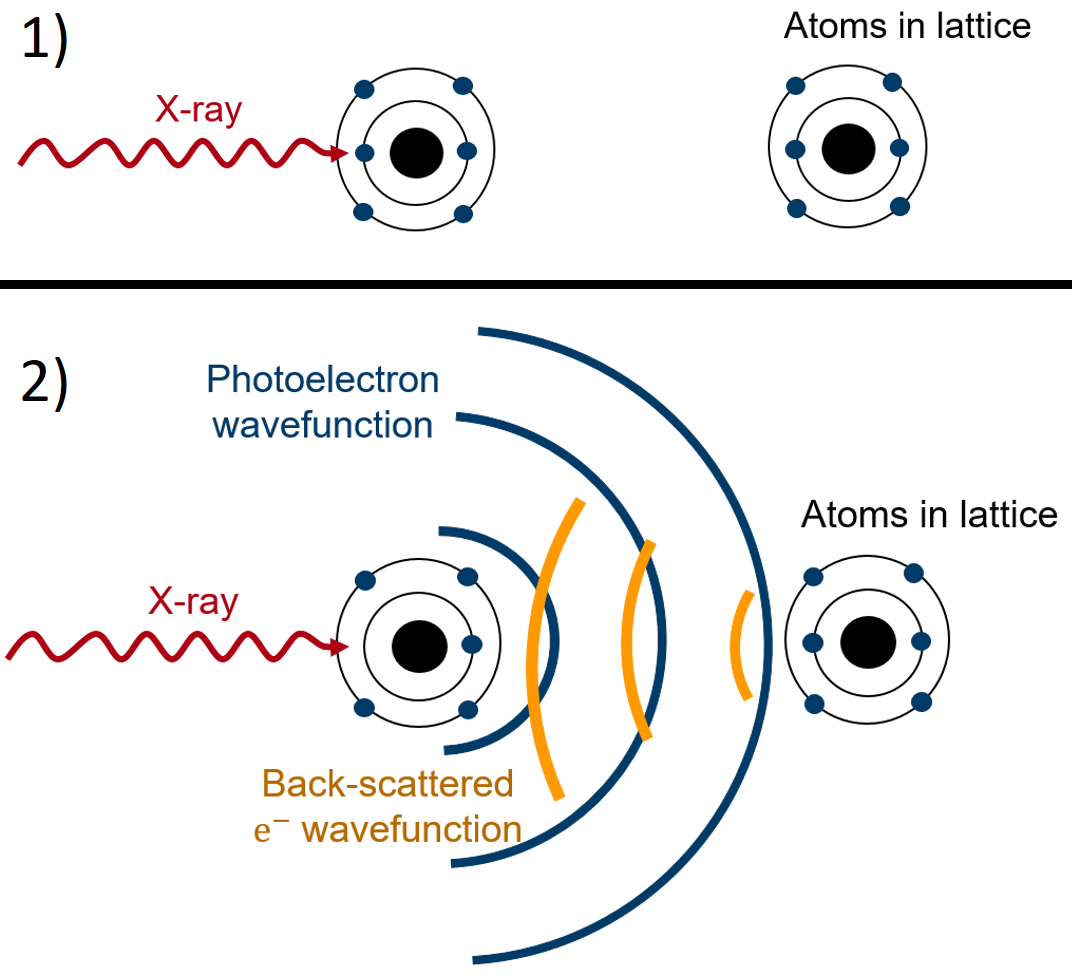
\includegraphics[width = 0.55\textwidth]{Diagrams/XAFS_scheme.PNG}
	\caption{Schematic representation of XAFS mechanism. 1) An electron is 
	ejected from the absorbing atom through the photoelectric effect. 2) The 
	electron wavefunction is partially back-scattered by a neighboring atom 
	in a lattice, which returns to the absorbing atom and modulates the 
	electronic states, consequently modulating the absorption coefficient.}
	\label{XAFS_scheme}
\end{figure}

XAFS can be broken 
down into two techniques: X-ray Absorption Near Edge 
Structure (XANES), covering the range of 
\SI{50}{\electronvolt} within the K-edge 
\citep{peyrusse2009k}, and Extended X-ray Absorption 
Fine-Structure (EXAFS), extending as far as \eV{250} 
above the edge \citep{fontaine1979soft}. In the case 
of XANES, 
the shift and slope of the K-edge are governed by the 
degeneracy, ionization, and continuum lowering of the 
plasma and are affected by the electronic temperature and 
density  \citep{falk2018experimental, levy2009x}. For EXAFS, the amplitude of the absorption 
oscillations is an indicator of ionic temperature, while 
the 
position and frequency of the peaks reveal 
information about the density and ionic order 
\cite{riley2021warm}. Note that determining 
properties from the oscillations is more 
straightforward for EXAFS, as approximations of 
single scattering are valid in this region, 
simplifying theoretical models 
\citep{newville2014fundamentals}.

To give an idea of what XAFS absorption spectra typically look like and 
how WDM properties can be determined from them, I will summarize two 
experiments, with one applying XANES and the other EXAFS, whose results are 
depicted in fig. 
\ref{XAFS_examples}. In an experiment conducted by Levy\textit{ et al.} 
\citep{levy2009x} corresponding 
to fig. \ref{XAFS_examples}a, WDM of aluminum is produced through isochoric 
heating with a picosecond proton beam pulse generated by Target Normal Sheath 
Acceleration (TNSA) on gold targets. The sample is then irradiated with x-rays 
from a laser-driven plasma backlighter of erbium, allowing for recording of 
absorption spectra. By fitting theoretical models and simulations to the 
experimental near-edge curves, WDM quantities can be extracted. For example, the electron 
temperature is determined through the variable slope of the K-edge, where a 
steeper slope indicates a lower temperature. Likewise, the electron temperature 
can be found by studying the far-edge structures, as shown in fig. 
\ref{XAFS_examples}b. In this experiment by Torchio \textit{et al.} 
\citep{torchio2016probing}, iron samples are compressed and brought to WDM 
conditions through laser-driven shocks, then diagnosed with x-rays from a synchrotron beamline specialized for x-ray absorption 
techniques. The electron temperature is determined through comparison of the experimental EXAFS to theoretical models. In addition, information about the atomic structure of the sample 
is gained by studying the disappearance of certain peaks. Notable is also the 
decreasing amplitude of EXAFS oscillations with increasing temperature, which is 
indicative of a collapse of atomic order in the material. 

\begin{figure} [H]
	\centering
	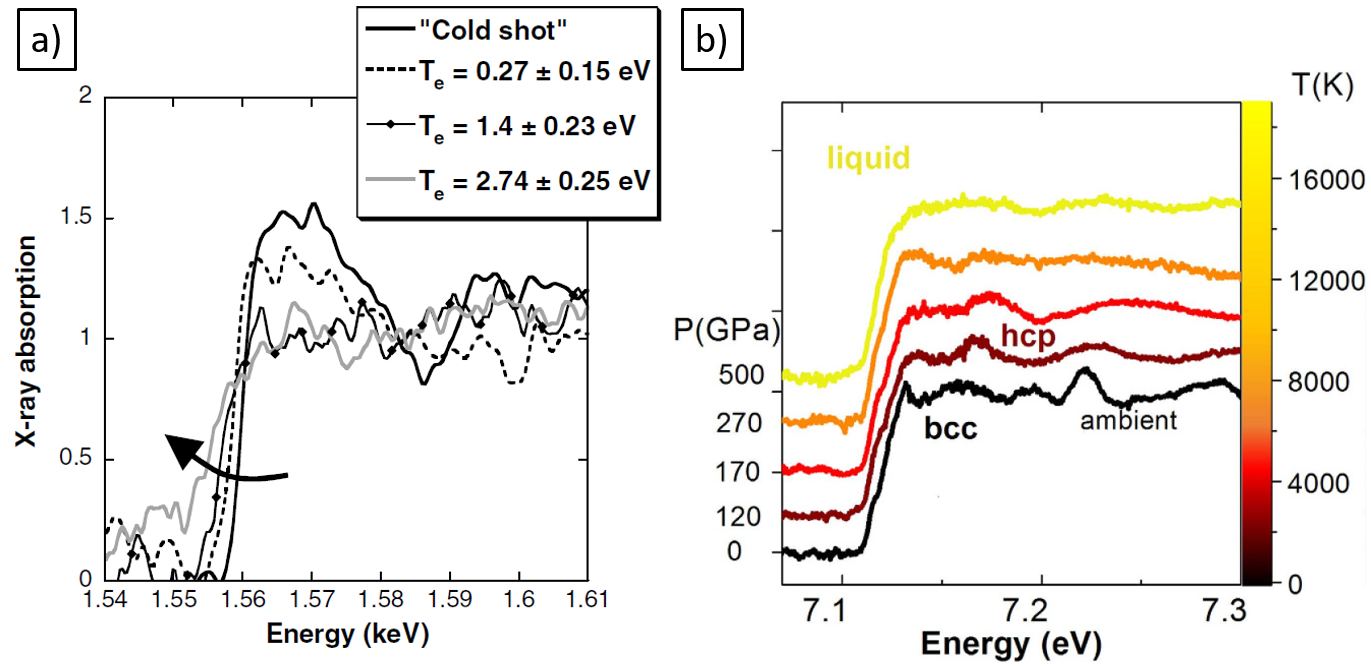
\includegraphics[width = \textwidth]{Diagrams/XAFS_examples.PNG}
	\caption{Examples of XAFS spectra taken in WDM experiments for XANES and 
	EXAFS respectively. It is important to note that the first graph displays 
	absorption spectra of aluminum, while the second shows spectra of iron. 
	\textbf{a)} Spectra from an aluminum sample isochorically heated to WDM 
	conditions with energetic proton beam and diagnosed with x-rays from 
	laser-driven plasma of erbium. XANES is applied to extract information 
	about the electron temperature \citep{levy2009x}. 
	The arrow highlights the reduction of the K-edge slope with rising 
	temperature.
	\textbf{b)} Spectra from an iron sample brought to WDM conditions with a 
	laser-driven shock and investigated with x-rays generated by a synchrotron. 
	EXAFS is conducted to derive the temperature and lattice structure of the 
	samples. Note that the spectra are artificially shifted along the y-axis to 
	represent rising pressure \citep{torchio2016probing}.}
	\label{XAFS_examples}
\end{figure}

Both of these results exemplify the power of XAFS as a diagnostic method for 
warm dense matter. As with most experiments in this vein, this method is made 
possible by x-ray spectrometers. Due to a number of restrictions originating 
from inherent properties of these devices and the volatile nature of WDM, the design of these spectrometers is essential for experimental success. As such, I will 
go into more depth on their history and design in the following chapter. 
	\chapter{Fundamentals of X-Ray Spectrometers}
\label{section: theory}

Since their inception in 1914 \citep{bragg1914x}, x-ray spectrometers 
have 
developed into an indispensable tool for plasma and high-energy 
density matter 
research, where x-rays allow probing into the optically opaque samples \cite{renner2019challenges}. This can be attributed in part 
to the 
unique challenges presented by x-rays and their interaction with 
matter. 
Conventional optics cannot be applied, as no absorption free 
materials are 
available and sufficient reflectivity is only achieved with 
grazing-angle 
incidence, greatly increasing optical aberrations 
\citep{kunze2009introduction}. By necessity, the entire optics of 
the 
spectrometers must therefore be realized using as few components as 
possible. 
In most cases, this limits the components to two; the 
detector and the dispersive element, which spatially separates the 
photons 
according to their energies and in most cases consists of one 
reflecting 
surface, as each new surface reduces the intensity of the x-rays on 
detector. Additionally, the placement of the components in relation to the x-ray source plays a vital role. In light of these limitations, x-ray spectrometers 
are generally designed with the specific experimental scheme and 
goals in mind 
and optimized using ray-tracing codes \citep{renner2019challenges}.

Central to the function of these spectrometers is the dispersive 
element. For 
energies below \eV{250}, gratings are 
generally used, 
owing to their high reflectivity, while for x-rays from 
\eV{250}-\SI{100}{\kilo\electronvolt}, and 
therefore for this work, crystals are more suitable
\citep{renner2019challenges}. The spectral dispersion of the x-rays 
occurs upon 
reflection on the 
dispersive element, where optical path differences between incident 
photons 
lead to interference. If this difference corresponds to multiples of 
the 
photon's wavelength, there is constructive interference, while the 
reflected 
intensity of other wavelengths is suppressed. As the optical path 
difference 
depends on the incident angle, photons are dispersed according to 
wavelength. 
In the case of crystals, this dependence is expressed by Bragg's law 
\citep{yang2011focusing}
\begin{equation}
	n\lambda = 2d_l\sin(\theta),
	\label{Bragg}
\end{equation}
where $n$ is the diffraction order, $\lambda$ the wavelength, $d_l$ 
the lattice 
constant, and $\theta$ the grazing angle.

In this work I will categorize the wide variety of spectrometer 
designs into 
two types; flat crystal and bent crystal spectrometers. Crystals can be 
one-dimensionally 
bent, for example cylindrically, or two-dimensionally, i.e. 
conanically or 
spherically. The type and degree of bending is limited by the 
crystal material 
and available production methods \citep{kunze2009introduction}. 
Typically, flat 
crystal spectrometers 
offer simplicity, ease of build, and more diverse crystal material choice 
with fewer 
defects, while bent crystal spectrometers exhibit the potential for combining dispersion and focusing in one element, yielding 
more 
flexible geometries and potentially high resolution and intensity 
on the detector 
\citep{renner2019challenges,kunze2009introduction}. As a result, 
improved 
signal-to-noise ratios are expected for bent crystal designs, at the 
cost of 
more complicated schemes and potential for crystal defects. 

In this section, I aim to introduce the background and fundamentals 
needed for 
this work. First in section 2.1, the flat crystal design is briefly 
outlined 
and 
explained, also serving as a baseline used to introduce some 
important 
quantities. In section 2.2, bent crystal designs are discussed, 
including an 
overview of the von-Hamos geometry and a more detailed 
explanation of the Focusing Spectrograph with Spatial Resolution (FSSR) 
geometry. Then, in section 2.3, the 
calculations for the dispersion of the spectrometer geometries designed in this work are shown. Lastly, the influences on the resolution are discussed in 
section 2.4.


\section{Flat Crystal Geometries}
\label{section: flat crystal geometry}

An example of a flat crystal spectrometer geometry is shown in fig. 
\ref{BasicSpec}, where the Bragg angle of the central energy, corresponding to 
the ray incident on the center of the detector, is given as 
$\theta_0$ and a Bragg angle of an arbitrary wavelength as $\theta$. For every 
incident angle on the crystal, only one wavelength fulfills the Bragg 
condition, so that the rays are dispersed on the detector with a dispersion 
$d(E)$, where $d$ gives the location of the rays on the detector. 
This 
dispersion equation is essential for processing of the spectra from 
raw data, and is 
therefore to be calculated or, for more elaborate geometries, 
determined using 
ray-tracing procedures.

\begin{figure}[H]
	\centering
	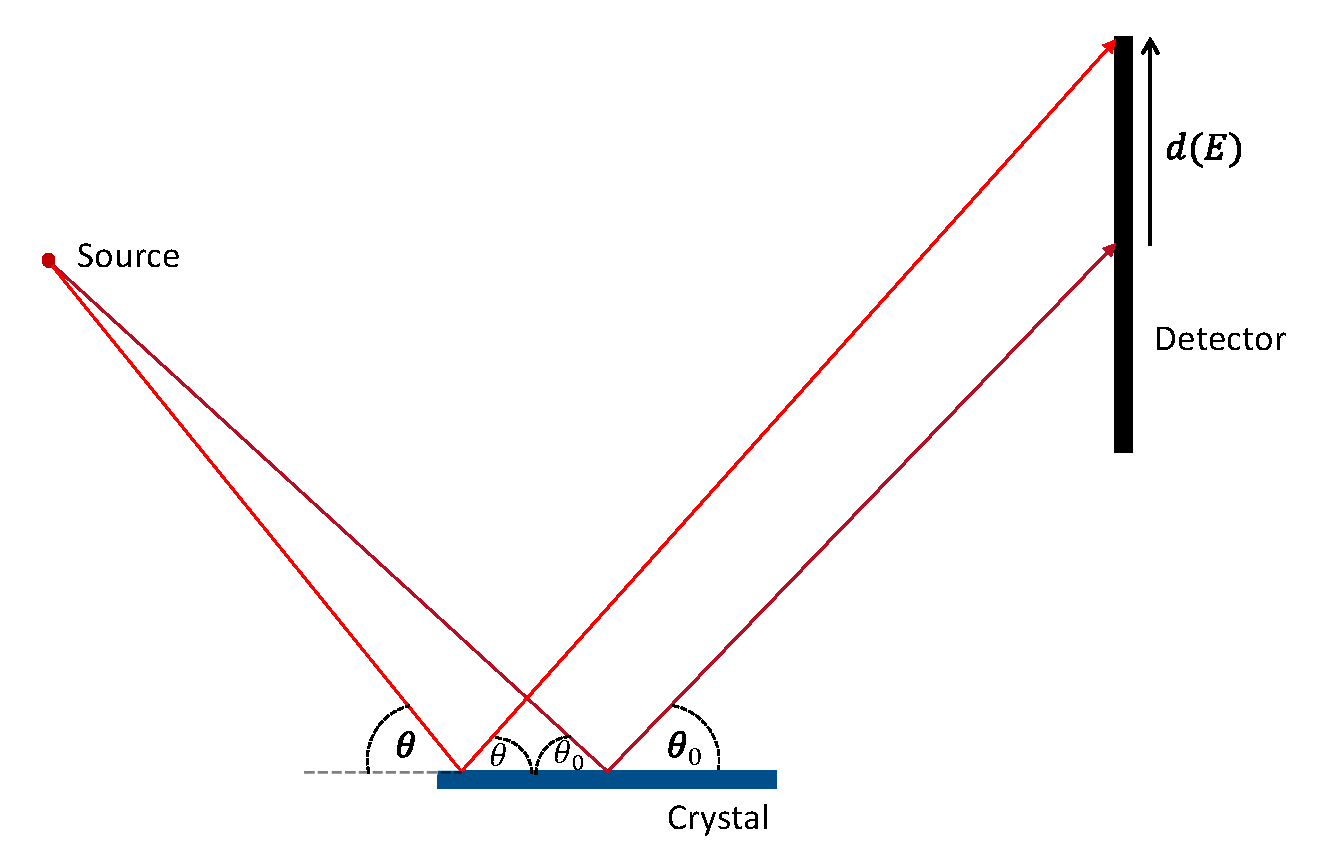
\includegraphics[width = 0.70\textwidth]{Diagrams/Basic_Spectrometer.pdf}
	\caption{Schematic geometry of a spectrometer with a flat crystal.}
	\label{BasicSpec}
\end{figure}

Currently, flat crystal spectrometers are typically eschewed in 
favor of bent 
crystal in the context of high-energy density matter experiments, 
attributed to 
the higher intensity on detector and reduction of source-size 
influences on the 
resolution of bent crystal schemes. If flat crystal schemes are 
used, they 
often come in as compact, easy-to-use mini-spectrometers, mostly 
serving 
supportive roles \citep{renner2019challenges}. Notably, a novel 
type of flat 
crystal spectrometers shows promise, employing two vertically 
orientated plane 
crystals, but is not suitable for this work due to its lower 
collection 
efficiency \citep{renner1999vertical}. Nevertheless, flat 
crystal 
schemes could prove suitable if the experimental scheme covers the 
drawbacks, 
i.e. small source size and intense x-ray source, and a simple 
spectrometer 
scheme with fewer crystal artefacts is desired.

\section{Bent Crystal Geometries}

Bending of the 
crystal allows for higher intensity on the detector, and therefore 
better 
signal-to-noise ratios, as the crystals collect the rays more 
effectively than 
their flat counterparts. Intuitively, this can be understood as more 
surface area of the crystal reflecting light of a certain wavelength 
onto the 
same approximate region on the detector. This comes at the cost of 
possibly 
worsening intrinsic reflection properties of the crystal 
\citep{holzer1998flat}, potentially impacting the inherent resolution due to the 
crystal, 
though the focusing properties of the scheme can 
offset this 
impact \citep{renner2019challenges}. Spherical crystals often entail 
FSSR 
geometries, while cylindrical crystals are applied for von Hamos 
geometries. Both will be handled individually in 
the 
following, with a more detail explanation of the FSSR, which is the geometry used in this work. 

\subsection{Von Hamos Geometry}

The von Hamos geometry is shown schematically in fig 
\ref{SchematicVonHamos}. 
In this case the 
components are placed such that the source and detector lie on the 
cylinder 
axis of the crystal. As a result, all rays emitted from a point 
source with the 
same incident angle on the crystal are focused onto the same point 
on the 
detector, regardless of 
where they are reflected on the circular arc. In effect, the 
geometry leads to 
one dimensional imaging of the source, with the spatial resolution 
along the y 
axis 
and spectral resolution in x direction in fig 
\ref{SchematicVonHamos}. With its 
high collection efficiency and 1-D imaging, this scheme is popular, 
but has the 
drawback of a shallow angle of incidence on the detector and 
sensitivity to 
source broadening in the dispersive direction 
\citep{renner2019challenges}.

\begin{figure}[H]
	\centering
	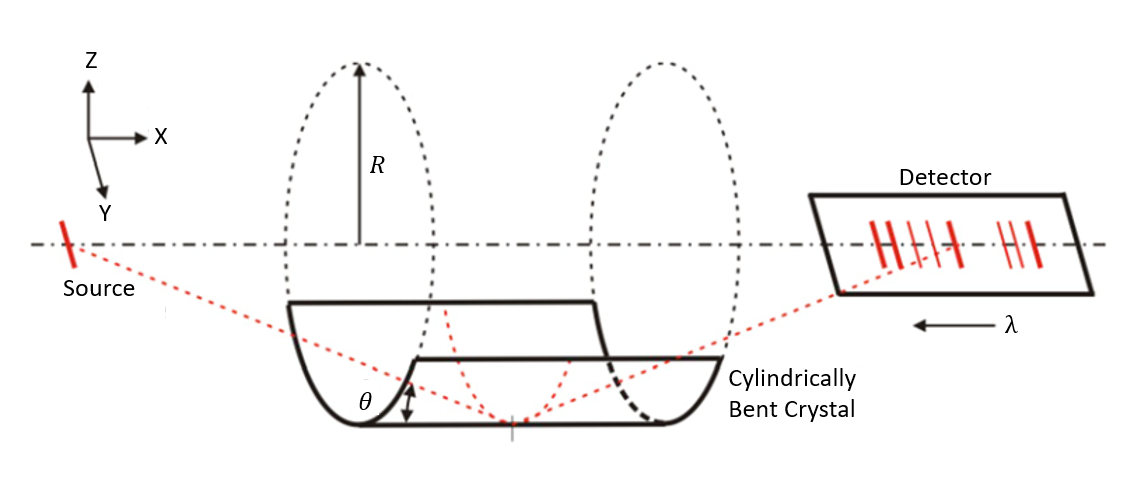
\includegraphics[width = 
	0.90\textwidth]{Diagrams/Schematic_vonHamos.PNG}
	\caption{Schematic representation of a spectrometer of the von 
	Hamos 
	geometry. R represents the crystal curvature radius. 
	\citep{renner2019challenges}}
	\label{SchematicVonHamos}
\end{figure}



\subsection{Focusing Spectrograph with Spatial Resolution} 
\label{SectionTheoryFSSR}

The FSSR has become 
one of the most widely used spectrometer geometries in plasma diagnostics 
\citep{yang2011focusing}, since it offers high luminosity, spectral and spatial 
resolution, and can cover relatively large energy ranges \citep{renner2019challenges}. Its geometry is 
characterized by the 
use of a spherically bent crystal and is commonly separated into two variants, 
the FSSR-1D and 
FSSR-2D, whereby the suffix refers to the dimensions of the source imaging 
\citep{renner2019challenges, blasco2001portable}. Due to its comparable 
simplicity, the function 
of the FSSR-1D will first be described, followed by the FSSR-2D in the final 
paragraph.

Before discussing further, I need to make an aside about the terminology used 
here. When I refer 
to "imaging", I mean imaging in the sense of rays coming from an object plane 
being reflected in such a way that an 
image is formed in the image plane, 
which depends on from where the rays were emitted. This is analogous to what 
occurs for 
lenses and curved mirrors, which is simply the result of 
refraction or reflection on a curved surface. Furthermore I will differentiate 
between 
"mirror imaging" and 
"pinhole imaging", referring to imaging due to mirror curvature in the first 
case and pinholes as in pinhole cameras in the second. On 
the other 
hand, "spectral focusing" refers to the focusing of the rays of the same 
wavelength, but from 
different origins, onto a single point. This is in essence different from 
imaging, since it does 
not inherently form an image, although both cases involve a form of focusing.

A schematic representation of the geometry can be found in fig. 
\ref{3DSchematicFSSR}. To explain the workings of the FSSR-1D, it is 
instructive to define two 
distinct planes, as the properties of the spectrometer change between them. In 
this work they are 
denoted as the dispersive 
plane, containing the direction of dispersion and the circle depicted in fig 
\ref{3DSchematicFSSR}, and the vertical plane, which is perpendicular to the 
dispersive plane and 
includes the detector surface. In the literature these planes are often 
referred to as the 
meridional (dispersive) and sagittal (vertical) planes 
\citep{yang2011focusing,renner2019challenges}. First, I will focus on the 
dispersive plane.


\begin{figure}
	\centering
	\begin{subfigure}[t]{0.58\textwidth}
		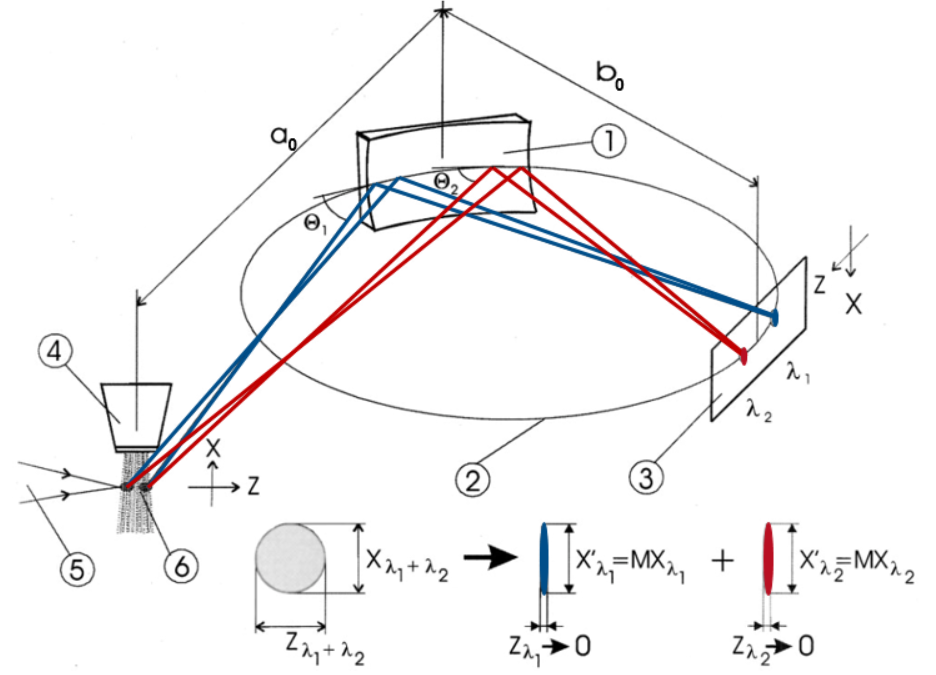
\includegraphics[width=\textwidth]{Diagrams/3DSchematicFSSR.PNG}
		\caption{Schematic depiction of the FSSR-1D spectrometer. (1) 
		Spherically bent crystal, (2) Rowland circle, (3) detector, (4) target 
		material (in the diagram a gas, in this work a foil), 
		(5) laser beam, (6) laser-produced plasma. Additionally the 
		imaging of the source is shown on the bottom, where a 1D-image is 
		formed for each wavelength. \citep{blasco2001portable}}
		\label{3DSchematicFSSR}
	\end{subfigure}%
	\hfill
	\begin{subfigure}[t]{0.38\textwidth}
	\centering
		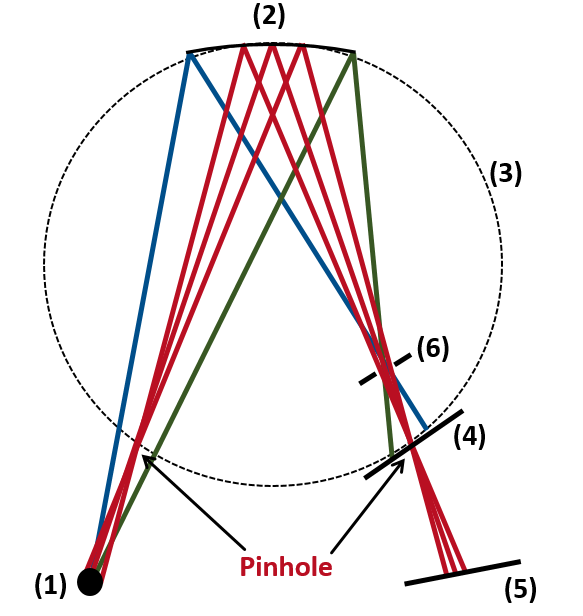
\includegraphics[width=\textwidth]{Diagrams/2D1DFSSR.PNG}
		\caption{Schematic comparison of the FSSR-1D and 2D configurations. (1) 
		Source, (2) 
		spherically bent crystal, (3) Rowland circle, (4) detector in FSSR-1D, 
		(5) detector in 
		FSSR-2D, (6) aperture at polychromatic crossover. Also pictured is the 
		location of the 
		pinhole-like points for the rays of a single 
		wavelength, here in red.}
		\label{FSSRComparison}
	\end{subfigure}
	\caption{FSSR Schemes.}
	\label{FSSRSchemes}
\end{figure}


An important concept to this configuration in the dispersive plane is the Johann 
geometry 
\citep{johann1931erzeugung}, which utilizes the so-called
Rowland circle (RC) (see fig. \ref{FSSRSchemes}), defined as a circle 
tangential to the spherical 
crystal at its midpoint with the radius $R/2$, where $R$ is the radius of the 
crystal 
curvature.  According to this geometry, any ray with a given wavelength that 
passes 
through a certain point on the RC fulfills the Bragg condition everywhere on 
the crystal surface and is focused in first approximation onto 
another point on the RC, mirrored across the crystal curvature pole. All other 
rays of this wavelength, which do not pass through this point, do not fulfill 
Bragg's law anywhere on the crystal and are hence not 
reflected. This effectively results in spectral focusing of the light onto the 
RC independent of where the rays are emitted, as schematically illustrated 
in fig. 
\ref{3DSchematicFSSR}, where the red and blue rays indicate different 
wavelengths. To note here is 
also that placing the detector on the RC is the defining feature of the FSSR-1D 
\citep{monot2002high}.

For both planes, mirror imaging properties are an additional important aspect originating from the spherical bending, comparable to imaging from a concave 
mirror and 
therefore in itself independent of wavelength. There are two focal lengths, one 
for each plane,  
which result from astigmatism due to the off-axis location of the source with 
respect to the 
crystal. The imaging condition, which follows from the mirror equation, in the 
vertical plane is 
\citep{blasco2001portable} 
\begin{equation}
	\frac{1}{a}+\frac{1}{b} = \frac{(2\cos(\alpha))}{R},
	\label{Sfocusing}
\end{equation}
where, for a given ray, the distance between emission point and crystal 
incidence is denoted as 
$a$, the distance between crystal incidence and detector incidence as $b$ and 
the Bragg angle as 
$\theta$, with $\alpha = 
90\degree - \theta$. To achieve the best 
possible spectral resolution and imaging, the source-crystal distance $a_0$, where the 
index 0 refers to the 
central ray, and the crystal-detector distance $b_0$ are chosen 
so that eq. \ref{Sfocusing} is satisfied \citep{blasco2001portable, 
renner2019challenges,faenov1994}. This ensures sharp imaging in the vertical 
plane. It is 
important to note that for the FSSR-1D, there is no imaging on the detector in 
the dispersive 
plane, as the detector lies on the point of spectral focusing. Despite this, 
the mirror imaging in 
the dispersive plane (see \citep{blasco2001portable}) does lead to a 
convergence of rays of 
different wavelengths onto a region between detector and crystal. By placing an 
aperture on this 
region, referred to as the polychromatic crossover (see fig. 
\ref{FSSRComparison}), extraneous 
rays are blocked, reducing the 
background on the detector \citep{renner2019challenges}. Through mirror imaging 
and spectral 
focusing, the FSSR-1D produces a series of 1D, spectrally distinguished images 
on the detector, as 
depicted in the bottom of fig. \ref{3DSchematicFSSR}. 

In the other variant of the FSSR, the FSSR-2D, the detector is placed anywhere 
not on the RC 
\citep{faenov1994}. If the detector and source lie outside of the RC, pinhole 
imaging for each 
wavelength is realized in the dispersive plane. The "pinholes" are a result of 
the spectral 
focusing and are located on the RC as labeled in fig. \ref{FSSRComparison}. A 
good way to imagine 
this is by removing everything inside the RC and bringing the "pinholes" 
together, forming a 
typical pinhole camera setup for each wavelength. Hence 
the magnification in the dispersive direction depends on the 
distance of the source and detector respectively to the RC 
\citep{renner2019challenges}. This pinhole imaging in the dispersive plane, 
along with mirror 
imaging in the vertical plane, results in a series of 2D spectrally selected 
images on the 
detector with different magnifications in each plane \citep{pikuz1995bragg}. In 
general, the 1D 
configuration yields the highest possible spectral resolution, since there is 
minimal overlap of energies due to spectral focusing, while the 2D setup allows 
for 2D 
quasi-monochromatic imaging of the source at the cost of reduced spectral 
resolution \citep{renner2019challenges}. Accordingly, the FSSR-2D setup is 
suitable for use with a 
source that emits a quasi-discrete spectrum, as a continuous spectrum would 
lead to a continuous 
set of 2D-images, leading to very low spectral resolution.




\section{Dispersion Calculation}
\label{section:dispersion calculation}
The dispersion $d(E)$ of x-ray spectrometers shows the relation between a spatial 
coordinate, in this work $d$ as defined in fig. \ref{DispersionDUCK}, and the energies $E$ of the photons. Therefore $d(E)$ 
quantifies where each photon with energy $E$ is expected to land on the 
detector dispersive line for a given spectrometer configuration. Generally 
speaking, an approximately linear dispersion is desirable, since it simplifies 
data processing and ensures an even spread of energies on the detector, so that 
no information is lost due to variable resolution \citep{yang2011focusing}. I 
will calculate the dispersion for the two geometries used in this work, 
namely for the flat crystal geometry found in fig. \ref{BasicSpec} and the 
FSSR as depicted in fig. \ref{FSSRComparison}. 

\subsection{Flat Crystal Geometry}

\begin{figure}[H]
	\centering
	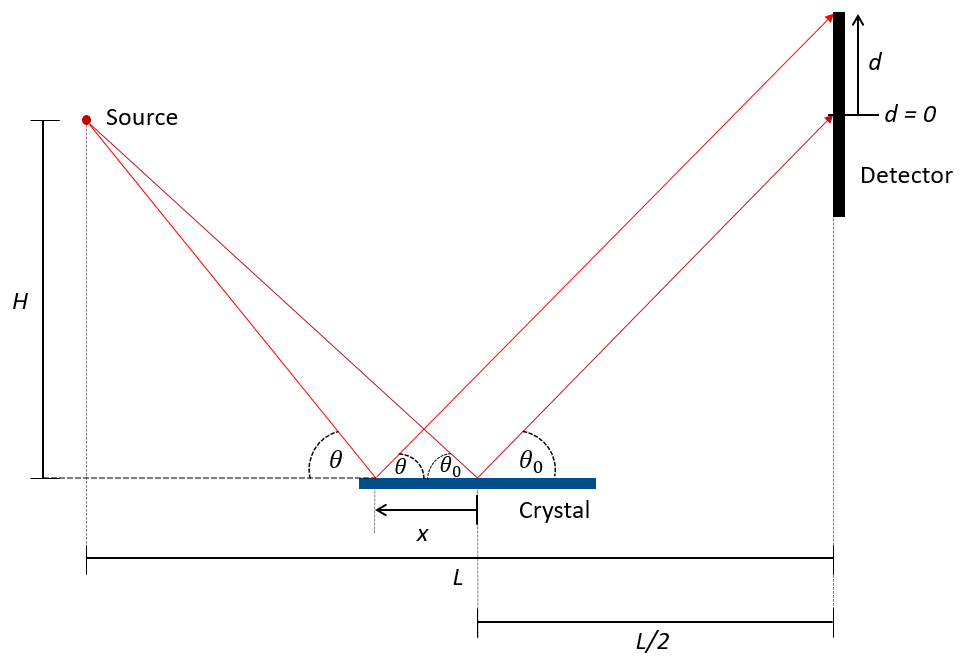
\includegraphics[width=0.8\textwidth]{Diagrams/DUCKDispersionCalc.PNG}
	\caption{Schematic representation of a flat crystal geometry with the 
	detector 
	perpendicular to the crystal surface.  $d$ is 
	defined as lying on the intersection of the dispersive plane and detector 
	surface, with its origin on the location of the central ray, corresponding 
	to $\theta_0$, on the detector. x is the distance between the 
	incident points
	of a given ray and of the central ray on the crystal in the dispersive 
	plane. H is the height of the spectrometer, i.e., the vertical distance 
	from 
	the 
	source to the crystal surface, and L is the length of the 
	spectrometer, i.e., the source-detector distance.}
	\label{DispersionDUCK}
\end{figure}

I will calculate the dispersion for the flat crystal configuration using 
trigonometry and the Bragg condition. The parameters used can be referenced 
from fig. \ref{DispersionDUCK}. From the path of the non-central ray in the 
diagram with the Bragg angle $\theta$, I get the two relations
\begin{subequations}
	\begin{align}
		\tan\theta &= \frac{H+d}{\frac{L}{2} + x} \label{eq:duckdispa} \\
		\tan\theta &= \frac{H}{\frac{L}{2}-x}. \label{eq:duckdispb}
	\end{align}
\end{subequations} 
Setting the right hand sides equal to each other and solving for $x$ yield
\begin{equation}
	x = \frac{L}{2}\cdot\frac{d}{d + 2H}.
\end{equation}
I then plug this into eq. \ref{eq:duckdispa} and simplify, 
which gives
\begin{equation}
\tan\theta = \frac{d}{L} + \frac{H}{\frac{L}{2}}.
\end{equation}
By identifying $\frac{H}{L/2} = \tan\theta_0$ and solving for $d$, I can write
\begin{equation}
d = L(\tan\theta-\tan\theta_0).
\end{equation}
Finally, using Bragg's law (see eq. \ref{Bragg}) and 
\begin{equation}
	\tan\theta = \frac{\sin\theta}{\sqrt{1-\sin^2\theta}} = 
	\frac{1}{\sqrt{1/\sin^2\theta - 1}},
\end{equation}
I receive the dispersion for the flat crystal geometry with detector 
perpendicular to the source
\begin{equation}
d(E) = L\left(\frac{1}{\sqrt{\left(\frac{2d_l}{nhc}\right)^2E^2 - 1}}  - 
\frac{1}{\sqrt{\left(\frac{2d_l}{nhc}\right)^2E_0^2 - 1}}\right),
\label{DispersionCalcDUCK}
\end{equation}
where $E_0$ denotes the energy of the central ray, $h$ the Planck constant and 
$c$ the speed of 
light, which is used in the conversion $\lambda = hc/E$. 
Consequently the dispersion is determined by four parameters in total: $n$, 
$d_l$, $E_0$ and $L$.

\subsection{Focusing Spectrograph with Spatial Resolution}

\begin{figure}[H]
	\centering
	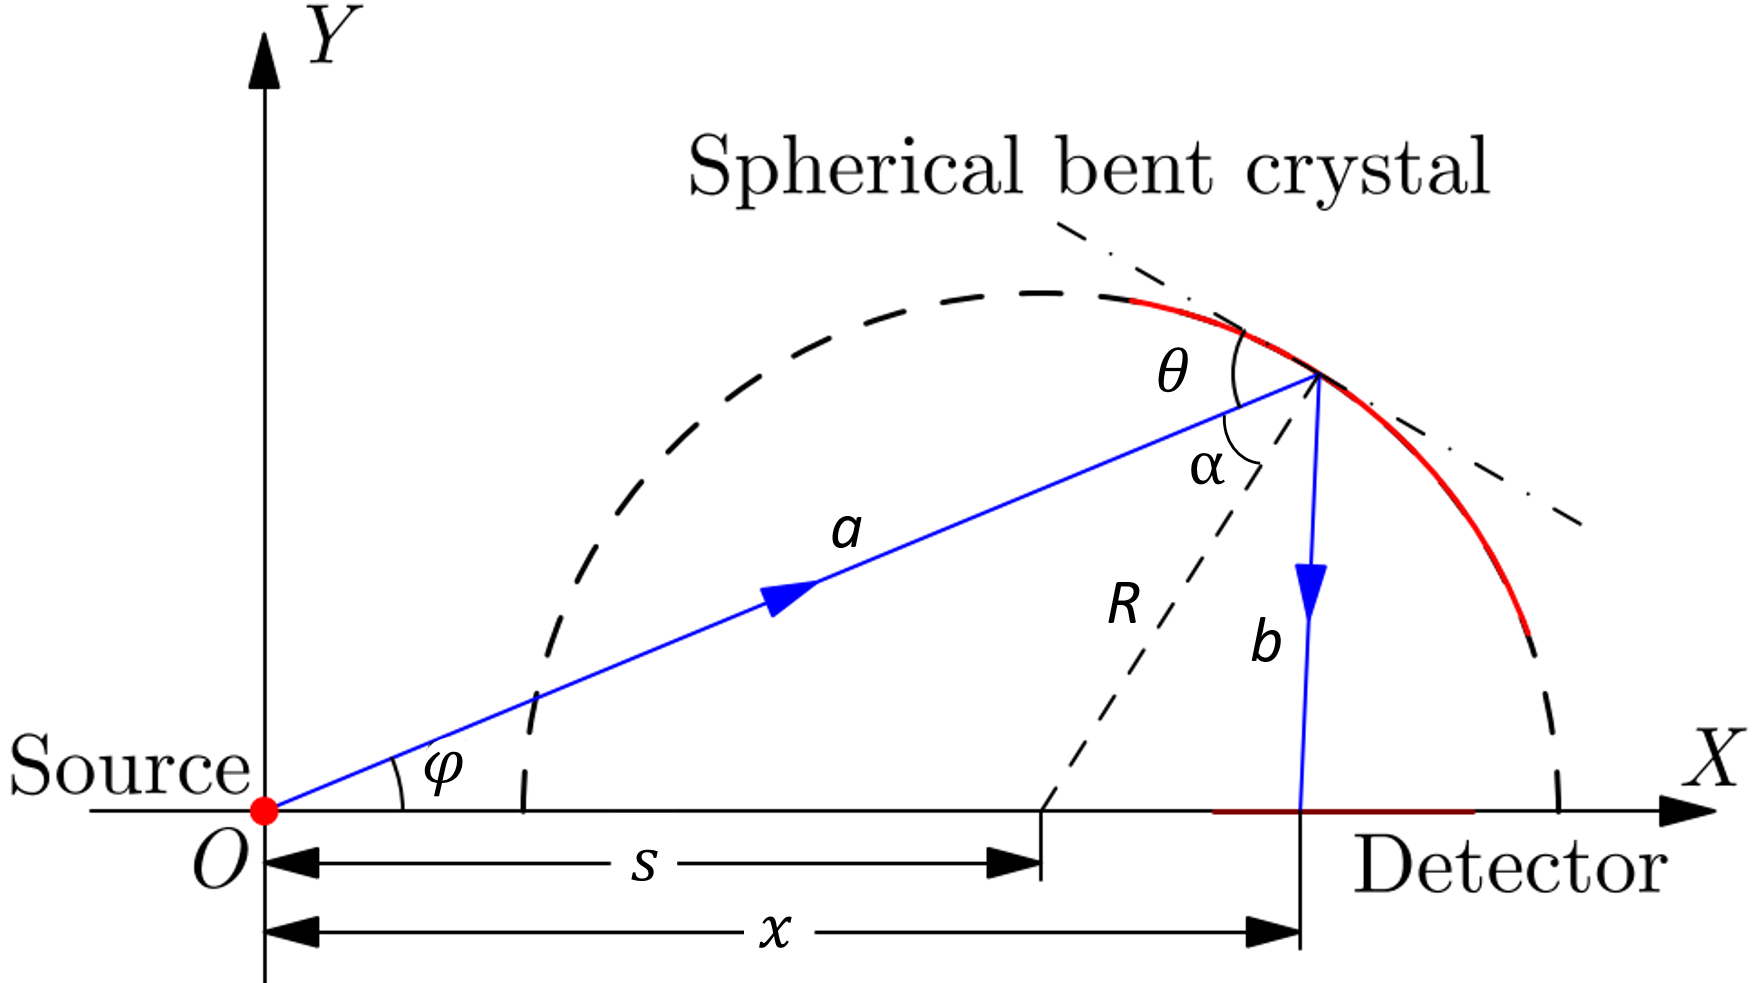
\includegraphics[width=0.8\textwidth]{Diagrams/FSSRDispersionYang.PNG}
	\caption{Geometry of an FSSR spectrometer, labeled with quantities useful 
		for analytical calculations. Note that this is generalized, so that 
		it's applicable for 
		both the FSSR-1D and 2D. \citep{yang2011focusing}}
	\label{DispersionFSSR}
\end{figure}

Before calculating the FSSR dispersion, it is important to consider a 
restriction on the detector position. The dispersion line on the detector 
surface, which corresponds to 
$d$, must lie on a symmetry axis of the sphere drawn out from the crystal 
curvature and point towards the source, so that the imaging condition in the 
vertical plane (see eq. \ref{Sfocusing}) is fulfilled for all photon energies. 
With this 
placement, the dispersion can be analytically calculated. \textit{Q. Yang et. 
al.} 
\citep{yang2011focusing} carried out this calculation employing the coordinate 
system and 
quantities found in fig. \ref{DispersionFSSR}. For the dispersion 
$x(\varphi(\theta))$ they found
\begin{equation}
	x = \frac{2s\chi(\chi+s\cos\varphi)}{\kappa},
\end{equation}
where
\begin{equation}
\begin{gathered}
	\chi = (R^2-s^2\sin^2\varphi)^{1/2} \\
	\kappa = 2\chi^2 + 2s\chi \cos\varphi - R^2. \label{eq:kappa}
\end{gathered}
\end{equation}
To bring $x(\varphi)$ into the form $d(E)$, I first express $\chi$ and 
$\kappa$ in terms of $\alpha$, which is related to the Bragg angle $\theta$ 
through the equation $\alpha = 90\degree - \theta$. By taking advantage of the 
triangle traced out by $R$, $a$ and $s$, I can write
\begin{equation}
	\begin{aligned}
		\chi &= R\cos(\alpha)
		\\ \cos\varphi &= \frac{(a - R\cos\alpha)}{s}
	\end{aligned}
\end{equation}
Plugging this into eq. \ref{eq:kappa} leads to 
\begin{equation}
	\begin{aligned}
		\kappa &= 2R^2\cos^2\alpha + 2sR\cos\alpha \cos\varphi - R^2
		\\& =  2R^2\cos^2\alpha + 2sR\cos\alpha \frac{(a-R\cos\alpha)}{s} - R^2
		\\& =  2Ra\cos\alpha - R^2.
	\end{aligned}
\end{equation}
From this and $s = \sqrt{a^2+R^2-2aR\cos\alpha}$ follows 
\begin{equation}
	x(\theta) = \frac{\sqrt{a^2+R^2-2aR\sin\theta}}{1-\frac{R}{2a\sin\theta}},
\end{equation}
where $\cos\alpha = \sin\theta$ was used. The only implicit dependence on 
$\theta$ left in this equation is in $a(\theta)$. Using the same triangle from 
above and the fact that $s$ is independent of $\theta$, $a$ can be written as
\begin{equation}
	\begin{gathered}
		a = R\sin\theta+\sqrt{R^2\sin^2\theta + s^2 - R^2} \\
		\text{with }s = \sqrt{a_0^2 + R^2 - 2a_0R\sin\theta_0},
	\end{gathered}
\end{equation}
where $a_0$ and $\theta_0$ denote these values for the central ray. Note that 
for simplicity $a_0$ and $\theta_0$ were chosen to calculate $s$, though any 
combination of $a$ and $\theta$ can be used. To determine $d(E)$, I introduce a 
coordinate transform according to fig. 
\ref{DispersionFSSR} with $x_0 = x(\theta_0)$. In the case of a FSSR-1D 
geometry, $x_0$ is equivalent to $a_0\sin(2\theta_0)$, owing to the right angle 
of the central ray with the detector surface. Accordingly $d$ can be written as
\begin{equation}
	d = x - x_0.
\end{equation}
Applying this transform, Bragg's law as in eq. \ref{Bragg} and converting from 
$\lambda$ to $E$ as 
before finally yields
\begin{equation}
	d(E) = \frac{\sqrt{a^2+R^2-\frac{2Rnhc}{(2d_l)} \cdot 
	\frac{a}{E}}}{1-\frac{R(2d_l)}{2nhc}\cdot\frac{E}{a}} - x_0,
	\label{DispersionCalcFSSR}
\end{equation}
where
\begin{equation}
	\begin{gathered}
	a = 
	\frac{Rnhc}{(2d_l)}\cdot\frac{1}{E}+\sqrt{\left( 
	\frac{Rnhc}{(2d_l)}\right)^2\cdot\frac{1}{E^2}
	 + s^2 - R^2} \\
	\text{with } s = \sqrt{a_0^2 + R^2 - \frac{2a_0Rnhc}{(2d_l)}\frac{1}{E_0}}.
	\end{gathered}
\end{equation}
Therefore, the quantities required to find the dispersion $d(E)$ of an FSSR are 
the 
crystal curvature radius $R$ and lattice constant $d_l$, diffraction order $n$, 
central photon energy $E_0$, central Bragg angle $\theta_0$ and source-crystal 
distance $a_0$. To note is that this result is applicable for both the FSSR-1D 
and 2D.



\section{Resolution}
\label{section: resolution theory}

In general, the resolution of a spectrometer mainly depends on three factors 
\citep{renner2019challenges,monot2002high}, which will be discussed in this 
section:
\begin{enumerate}
	\item Source broadening
	\item Intrinsic crystal properties
	\item Detector resolution
\end{enumerate}
Which of these has the greatest effect on the resolution depends on the choice 
of geometry, crystal and detector. 

Source broadening refers to the effect the physical size of the source has on 
the resolution. For example, in the flat crystal geometry a larger source 
corresponds to a larger area covered by x-rays of the same wavelength on the 
detector, 
leading to worse resolution. This factor is strongly dependent on the geometry 
and crystal shape. Generally, the resolution of flat crystal spectrometers is 
strongly affected by source broadening, while FSSR spectrometers suppress the 
influence of source size \citep{renner2019challenges}.

The crystal properties that mainly affect resolution are structural in nature. 
The crystal structure influence is parameterized by the 
rocking curve width $\Delta \theta$, which is given by the FWHM of the 
reflected intensity as a function of incident angle and depends on wavelength 
and polarization of the radiation, crystal perfectness and bending radius 
\citep{renner2019challenges, holzer1998flat}. The reflection properties, mainly 
affecting the intensity on detector, are 
assessed using the integrated reflectivity $R_{int}$, i.e., the ratio of the 
angular intensity 
$I(\theta)$ integrated over the range of diffraction angles around a Bragg 
angle $\theta_B \pm 
\Delta \theta$ and the incident intensity $I_0$ \citep{holzer1998flat}
\begin{equation}
	R_{int} = \frac{1}{I_0}\int_{\theta_B - \Delta \theta}^{\theta_B + \Delta 
	\theta} I d\theta.
\end{equation}
Both these quantities can be calculated using the dynamical theory of X-ray 
diffraction 
\citep{holzer1998flat}. With these 
quantities the effect of the crystal on the resolution can be 
estimated.

Another factor for the spectrometer resolution is the detector spatial 
resolution, which can be estimated simply by using the dispersion $d(E)$ and 
spatial resolution $dx$ of the detector. In this work, this takes the form of 
pixel density on a CCD camera and is often the limiting factor for FSSR spectrometers 
\citep{renner2019challenges, monot2002high}, though it should be calculated 
on a case to case basis, as geometry design choices also impact this factor. 

For geometries capable of imaging, one can differentiate between spatial and 
spectral resolution. The spectral resolution is given directly by the energy 
interval corresponding to the area covered on the detector by x-rays of the 
same wavelength, while the spatial resolution relates to the image of the source 
on the detector and is only limited by deviation from the imaging 
condition for different locations on the x-ray source, as well as by detector resolution.

In the case of the von Hamos geometry, the spectral 
resolution is sensitive to source broadening in both x and z directions, as 
depicted in fig. \ref{SchematicVonHamos}, while the spatial resolution along 
the y axis remains unaffected \citep{renner2019challenges}. For the FSSR-1D, 
the spectral 
resolution is independent of source size due to the spectral focusing in the 
dispersive plane, a property that applies for the spatial resolution in the 
vertical plane as well, owing to the large $a$ distance relative to the typical 
source size in laser plasma experiments. In the FSSR-2D scheme, the optimal 
spectral focusing condition is no longer met, therefore a finite source size 
leads to source broadening in spectral direction as well \citep{monot2002high}. A geometrical calculation of the 
impact of source size on spectral resolution for the FSSR scheme can be found 
in \citep{young1998high}. 














	\chapter{Spectrometer Design}
\label{chapter: spectrometer design}
The design and testing of the spectrometers in this work is in preparation for the eventual characterization of warm dense matter of aluminum at FAIR. The WDM will be generated by energy deposition using a heavy-ion beam, leading to isochoric and near-homogeneous heating compared to other techniques. Since WDM is opaque to visible 
light, x-rays will be used for the main diagnostics. In this case, the 
source will be laser-driven plasma as a backlighter of the sample, 
distinguished by its tunability, high-brightness, and small angular 
dependence of the emission. Together, the homogeneity of the x-ray source and WDM sample enhances the diagnostics in that approximately a single WDM 
state can be probed, reducing unknowns in the experiment. XAFS will be 
the diagnostic method of choice, a technique that notably enables 
measurements of optically-opaque short-lived non-crystalline matter, as discussed in chapter \ref{chapter: XAFS}. X-ray spectrometers are 
ubiquitous in WDM experiments using XAFS, and here is no exception. 

The design of the two spectrometers must accommodate each main 
aspect of the experiment. The heavy-ion heating places demands on the 
sample size to ensure homogeneity and induces large amounts of 
background, necessitating careful shielding. The spectrometers must also accommodate the chosen backlighter, since the x-ray intensity and spectral structure of the source influence the viability of the x-ray absorption spectra. Finally, the use of XAFS sets restrictions on the photon 
energy range of the spectra and the resolution, as the features must be 
detected and resolved. The details of all these design considerations 
will be discussed shortly in the next section.

In this chapter I will discuss the designs of 
the spectrometers and their rationale, outlining the advantages and 
disadvantages of each. In section \ref{section: design considerations}, I 
will describe the considerations that informed the 
designs. Then in section \ref{section: spectrometer geometries}, the schemes of each 
spectrometer will be introduced in detail, along with short descriptions of two additional spectrometers designed by Philipp Hesselbach and used in the 2023 laser-only experiment. Finally in section \ref{section: specs and comparison}, the specifications 
of the spectrometers will be given and a comparison carried out, 
summarizing the purpose of each design.

\section{Design Considerations}
\label{section: design considerations}
For the design of the spectrometers I took five main 
considerations into 
account, which follow from the specific needs of the experimental setup:
\begin{enumerate}
	\item \textbf{Energy Range:} As stated in 
	the introduction, the main function of the 
	spectrometers is to perform X-ray Absorption 
	Fine Structure (XAFS) spectroscopy and 
	resolve the aluminum K-edge at 1558.98 
	\unit{eV} \citep{henke1993x} and its 
	features. Near edge structures 
	(XANES) can be observed within 
	50 \unit{eV} of the edge 
	\citep{peyrusse2009k}, while extended 
	fine 
	structures (EXAFS) can be measured as far 
	as 250 eV above the Al K-edge 
	\citep{fontaine1979soft}, which consist mainly of 
	several oscillations in the absorption 
	coefficient 
	\citep{levy2010double}. This yields an energy 
	range of approximately 1530 - 
	1810 \unit{eV}, where the upper value is much
	less strict than the lower and the lower value is 
	adjusted upward if the spectral range of the 
	spectrometer is mainly the immediate area of the 
	K-edge.
	\item \textbf{Sample Size:} The future heavy ion beam heating, 
	although more homogeneous than other WDM production methods, still 
	is partly inhomogeneous, since the energy deposited along the 
	heavy ion beam propagation direction, denoted 
	here as z, is not constant. This negatively impacts the absorption spectroscopy as the photons are dispersed in z-direction (see fig. \ref{BraggConstraint}), therefore x-rays of different energies probe slightly different conditions. If the conditions differed too much, the  interpretation of the XAFS spectra would be complicated, e.g. when oscillations over a large energy interval should be used for temperature measurements. Therefore, the previous considerations impose an upper limit on the sample size in z-direction. Furthermore, it has to be placed sufficiently close to the backlighter such that all detected X-rays can transmit through the sample, while a minimum distance has to be maintained for target design considerations and ion beam clearance. Here, we have chosen a sample-source distance of \SI{5}{\milli\meter} and a sample size in z direction of $\leq\SI{1}{\milli\meter}$, which must cover all detected X-rays (see fig. \ref{BraggConstraint}). Together this leads to a constraint on the central Bragg angle. It cannot be too large, 
	because, assuming a fixed energy range, a larger 
	$\theta_0$ requires a larger range of angles to 
	cover all the 
	energies compared to a 
	smaller $\theta_0$. This is due to the 
	proportionality $\lambda \propto 
	\sin\theta$, in which larger wavelengths have 
	smaller slopes. 
	\begin{figure}[H]
		\centering
		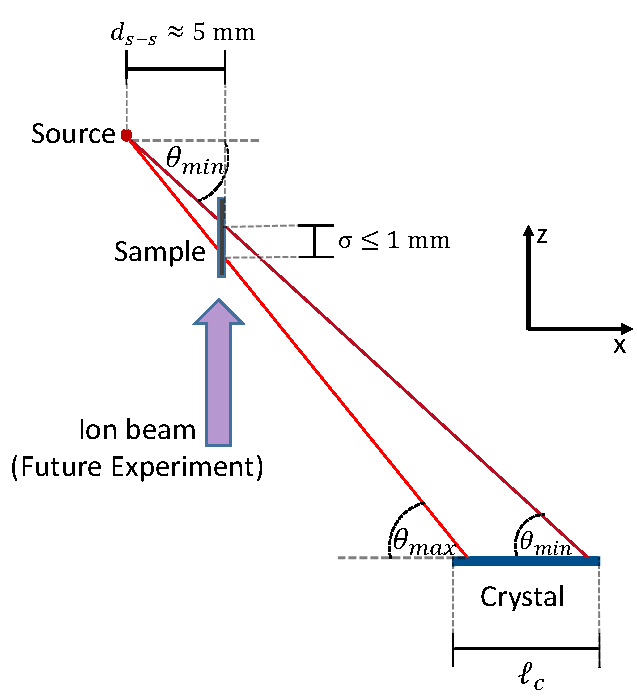
\includegraphics[width = 0.50\textwidth]{Diagrams/BraggAngleConstraint.pdf}
		\caption{Illustration of the sample size
			consideration. The length on the sample covered by x-rays in z direction 
			is denoted by 
			$\sigma$, which must stay at 
			or below \SI{1}{\milli\meter}. $\theta_{max}$ and 
			$\theta_{min}$ correspond to the 
			maximum and minimum Bragg angles of the 
			spectrometer respectively, while $\ell_c$ 
			represents the length of the crystal in the 
			dispersive plane and $d_{s-s}$ the source-sample 
			distance.}
		\label{BraggConstraint}
	\end{figure}
	\item \textbf{Spectral Resolution:} The main 
	requirement on the spectral resolution is 
	that it be high enough to resolve XAFS structures. From the example 
	spectrum given in fig. \ref{XAFS_examples}a, the required 
	resolutions can be estimated. Practically, 
	a spectral resolution of $\leq\SI{1}{\electronvolt}$ is expected to resolve the Al K-edge 
	sufficiently to carry out XANES, while $\sim$ 
	\SI{10}{\electronvolt} is required for EXAFS, estimated from 
	half of an oscillation period 
	\citep{levy2010double}. Spatial resolution 
	is 
	advantageous, but not a hard requirement. 
	\item \textbf{Intensity:} A high enough 
	intensity to resolve the spectra and perform 
	the absorption spectroscopy is necessary. In 
	the design this comes into play in part 
	through the length of the spectrometer and 
	distance to the source. Additionally the 
	choice of geometry and crystal play a role.
	\item \textbf{Physical Size:} The 
	spectrometers must fit in the HHT chamber. 
	This restricts the physical length to under 
	0.55 \unit{m}. There must also be space for the 
	heavy ion 
	beam in future experiments 
	and the PHELIX beam. 
\end{enumerate}


\section{Implemented Spectrometer Schemes}
\label{section: spectrometer geometries}
I designed two configurations according to the 
considerations above and the aspects discussed in the introduction to 
this chapter, namely a flat 
crystal geometry (see fig. \ref{BasicSpec}) 
and 
a bent crystal scheme, specifically a FSSR-1D geometry (see 
fig. \ref{FSSRSchemes}). For the flat crystal 
spectrometer, inspiration was 
drawn from \textit{Levy et. al.} \citep{levy2010double} and a dual channel 
geometry was chosen, so 
that both the transmitted and source spectrum can be 
simultaneously measured on a single detector. A flat crystal design has 
the advantage of simplicity in design and analysis of the spectra.

As for the bent crystal scheme, the 
FSSR-1D geometry offers the highest possible spectral 
resolution of FSSR schemes while also giving 
high luminosity on the detector. Additionally, it has the 
potential for 
1D imaging in the 
vertical direction, which could be exploited to 
simultaneously observe the 
source and transmitted spectra. I also considered a 
FSSR-2D configuration, but 
decided against it because some source spectra are 
expected to be smooth, 
which would significantly impact the spectral 
resolution. A von Hamos geometry was discarded because of its 
aforementioned shallow incidence angle on 
the detector, in contrast to the preferred quasi-perpendicular incidence on a CCD camera, and sensitivity to source 
broadening, 
which is altogether absent in the FSSR-1D scheme. 

The crystals for each scheme were chosen according to the considerations 
listed in the appendix, section \ref{section: crystal}, where the available crystal material choices and geometries influence each other so that a compromise must be found. In the end, I 
decided on using
ammonium dihydrogen phosphate (ADP) for the flat crystal geometry and 
mica for the bent crystal. ADP was 
chosen mainly for
its potential to reach 
extremely high optical and structural perfection as well 
as its lattice spacing of $2d_l = 
\SI{10.64}{\angstrom}$, allowing for diffraction in 
the first order, covering the 
desired energy range 
\citep{ferrari2019characterization, 
rajesh2015growth}. Mica was chosen for the FSSR-1D geometry for 
its bendability, high spectral 
resolution in tandem 
with good 
reflectivity, a wealth of previous applications in the 
literature and the possibility to use a low 
diffraction order (second order), yielding $2d_l/n = 
19.84/\SI{2}{\angstrom} = 
\SI{9.92}{\angstrom}$.
\citep{monot2002high,renner2019challenges,faenov1994,blasco2001portable}.
 One 
drawback of the mica crystal was that it contains 
aluminum, which could lead to 
a drop in reflectivity at the Al K-edge, though the 
expected decrease in 
intensity is not significant enough to exclude mica 
\citep{alkhimova2016determination}. Mica is also often 
used in FSSR 
spectrometers with strong bending, reaching radii of 
down to 
\SI{100}{\milli\meter} \citep{monot2002high}.

In addition to the two main spectrometers of this work, I will introduce 
another simple flat crystal spectrometer scheme in section \ref{section: SUCC}, which shares the geometry of a single channel of the flat crystal spectrometer I designed and
whose purpose is to deliver a wide energy range overview spectrum of the 
x-ray source as a control. It uses a potassium acid phthalate (KAP) 
crystal. This crystal is commonly used in x-ray spectrometers and has a 
larger rocking curve width than ADP \citep{kunze2009introduction, 
loisel2016measurement}. As this spectrometer is straightforward and not 
of my design, I will only describe it briefly and give its 
specifications.


\subsection{Dual Unbent Crystal Spectrometer}
\label{section:DUCC design}

\begin{figure} [H]
	\centering
	\begin{subfigure}[t]{0.48\textwidth}
		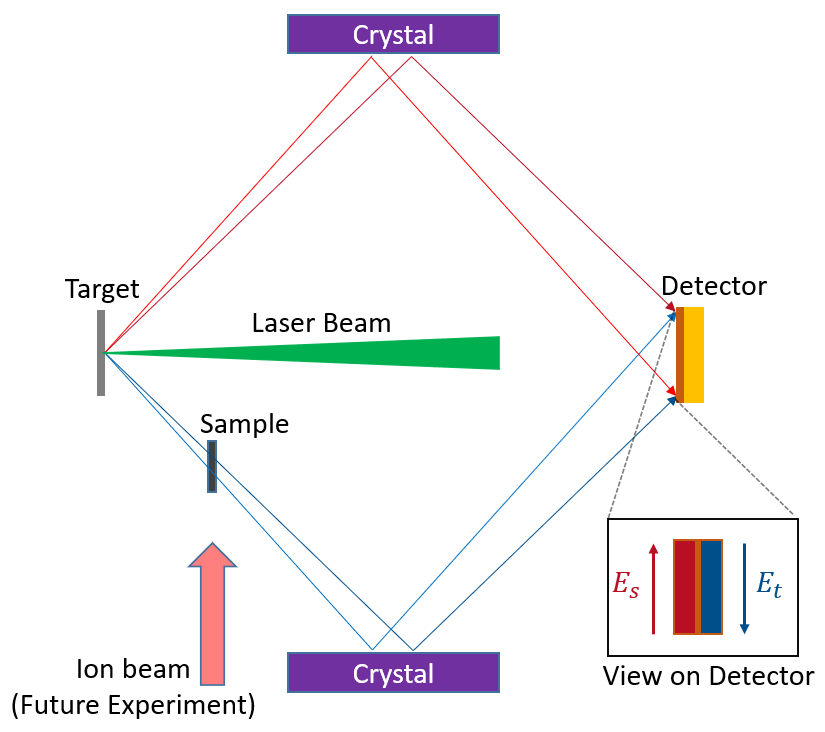
\includegraphics[width=\textwidth]{Diagrams/DUCCRealSchematic.PNG}
		\caption{Top view of the geometry, including a view on the detector which shows the detection of the source photons and transmitted photons with the energies $E_s$ and $E_t$, respectively.}
		\label{realDUCCSchematicTop}
	\end{subfigure}%
	\hfill
	\begin{subfigure}[t]{0.5\textwidth}
		\centering
		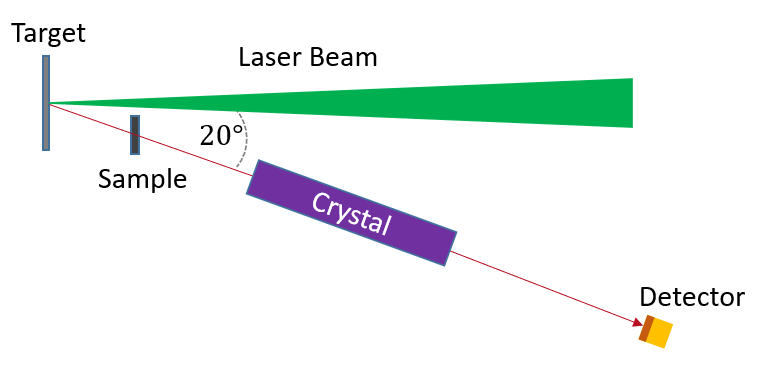
\includegraphics[width=\textwidth]{Diagrams/DUCCRealSchematicSide.PNG}
		\caption{Side view, in which the tilt of the 
			spectrometer is 
			illustrated.}
		\label{realDUCCSchematicSide}
	\end{subfigure}
	\caption{Schematic illustration of the DUCC geometry, not to 
		scale.}
	\label{realDUCCSchematic}
\end{figure}

The dual flat crystal spectrometer geometry, which I 
christened the \textbf{D}ual 
\textbf{U}nbent \textbf{C}rystal 
Spe\textbf{C}trometer (DUCC), is illustrated 
schematically in fig. \ref{realDUCCSchematic}. The 
central idea behind this 
geometry is to simultaneously record two spectra by 
implementing a mirror 
symmetrical two-channel design. This spatial symmetry 
ensures that the channels 
are illuminated by the same x-ray source, assuming a conical symmetry of the 
plasma emission. Through the combination of the DUCC geometry and ADP 
crystal, the DUCC spectrometer will target XANES and therefore 
have a relatively small energy range. This reduces the decrease of resolution due to source broadening and leverages the good crystal properties of the ADP.

In fig. \ref{realDUCCSchematicTop} the top view of 
the DUCC geometry is schematically shown. The laser beam 
irradiates the target, 
igniting a plasma. This plasma then emits soft x-rays, 
whose source spectrum is 
measured through the top channel using one half of the 
available detector 
surface. The transmitted 
spectrum through the sample, 
in this work an aluminum foil, is recorded through the 
bottom channel on the 
other half of the chip surface. The separation of the 
two spectra on the chip 
is realized by a plate with two openings inserted into 
the beam path before the 
two channels overlap (not shown in the figure). Space was 
left for the ion beam for 
future experiments, which 
is not a part of this work. To note is that 
space is left in the 
center of the spectrometer for a large lead block, which 
in the future will 
serve to shield the detector from protons being emitted from the sample due to the 
interaction with the heavy ion beam. Fig. 
\ref{realDUCCSchematicSide} depicts the $20\degree$ tilt 
of the DUCC spectrometer that I 
introduced to leave space for the laser beam, 
which is conical and has a half opening angle 
of $\pm 2.3\degree$. 
The 
spectrometer components 
were also tilted to simplify the design and deliver the 
simplest possible 
profile on the detector.




\subsection{Focusing Spectrograph with Spatial 
Resolution}

\begin{figure}[H]
	\centering
	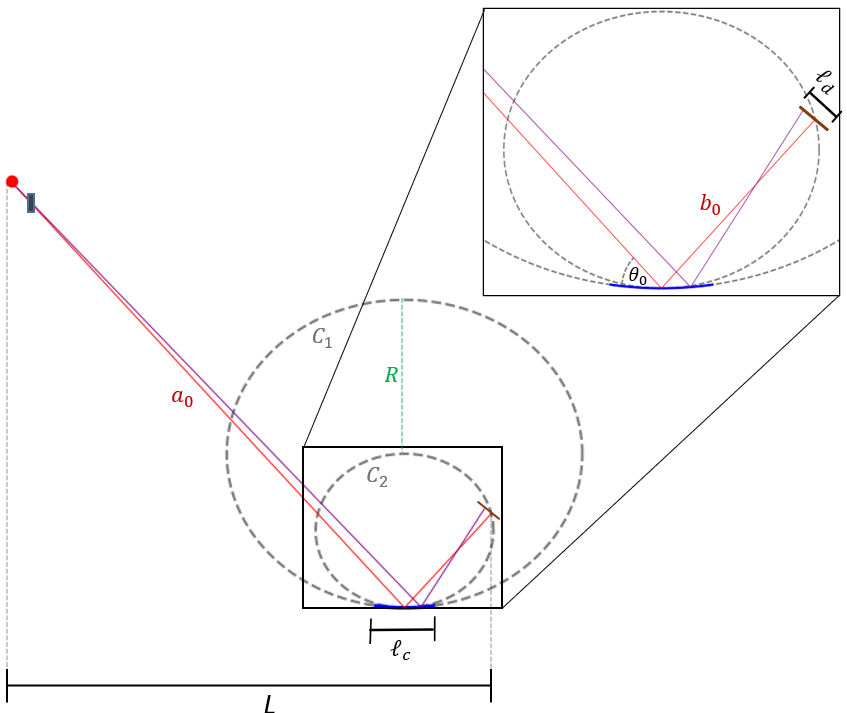
\includegraphics[width = 0.8\textwidth]{Diagrams/FSSRRealScheme.PNG}
	\caption{Schematic Illustration of the FSSR-1D, 
		where $R$ is the radius of curvature of the 
		crystal, $L$ the spectrometer length, $\ell_{c}$ 
		the length of the crystal in the dispersive plane 
		and $\ell_d$ the detector length in dispersive 
		direction. The crystal is depicted in blue, the 
		source in red and the sample in dark gray. Note 
		that the Rowland circle $C_1$ and circle drawn out by 
		the crystal curvature $C_2$ are also shown.}
	\label{realFSSRScheme}
\end{figure}

The FSSR-1D configuration used for the spectrometer with the curved crystal is 
depicted in fig. 
\ref{realFSSRScheme}. As the fundamental geometry 
effectively functions 
equivalently to the one 
described in section \ref{SectionTheoryFSSR}, I will 
not elaborate in detail on it here and instead discuss the spectrometer 
as a whole, 
so a FSSR-1D geometry with mica crystal. The main focus of this 
spectrometer is to capture a 
larger energy range, aiming to additionally resolve the oscillations in the 
EXAFS, 
while maintaining a good spectral resolution. 
Furthermore, the larger 
source-crystal distance $a_0$ and relation with the crystal-detector 
distance $b_0$ (see eq. \ref{Sfocusing}) allow freedom 
of placement in the chamber, as compared to the DUCC spectrometer. 
One 
potential drawback is 
the necessity of careful alignment and exact positioning 
of the components to 
achieve high spectral resolution, owing to the innate 
focusing and imaging of 
the FSSR scheme (see section \ref{SectionTheoryFSSR}). 

To note is that the potential of the 1D imaging for 
absorption spectroscopy with a single detector is not 
applied in this work due to the ratio of $a_0$ to $b_0$, 
leading to a magnification in the vertical plane of 
0.22. This magnification combined with the small 
sample size $\sigma$ renders an image too small to 
consistently differentiate between source and 
transmitted spectra. Despite this, the imaging 
properties find use in 
concentrating the x-rays from the plasma onto a 
single line in the dispersive direction on the 
detector, significantly reducing the effects of 
background, which will be especially advantageous in 
the future experiments with the heavy ion beam.

\subsection{Single Unbent Crystal Spectrometer}
\label{section: SUCC}
The \textbf{S}ingle 
\textbf{U}nbent \textbf{C}rystal 
Spe\textbf{C}trometer (SUCC) is a basic spectrometer, consisting of a 
single, flat crystal set in a geometry analogous to fig. \ref{BasicSpec} 
or to the top channel of the DUCC geometry (see fig. 
\ref{realDUCCSchematicTop}). Designed by P. Hesselbach, the spectrometer 
aims at a large enough energy range to cover both the FSSR-1D and DUCC 
spectrometer ranges, albeit at a lower resolution, owing to the source 
broadening intrinsic to the flat crystal geometry and the worse crystal 
properties of KAP as compared to ADP. To note is that the higher 
rocking curve width also increases the intensity on the detector, 
ensuring that control spectra are consistently recorded. Its role as a 
control implies that it will not be used for transmitted spectra.

In addition to the SUCC, another spectrometer by the name of old SUCC (OSUCC), a device used in a previous experiment and also designed by P. Hesselbach applying the same basic design as the SUCC, is used to extract spectra transmitted through a sample. The main purpose of the OSUCC in the experiment is to investigate the other aspects of the experimental setup by using an already tested spectrometer. In this work, it is used only when presenting qualitative results.

\section{Specifications and Comparison}
\label{section: specs and comparison}

For clarity and ease of discussion, I will for the rest of this work refer to the spectrometers by their geometries, i.e. DUCC, FSSR, SUCC, and OSUCC, where FSSR and FSSR-1D are interchangeable. If I specifically mean the geometries, I will append "geometry" onto the name, e.g. DUCC geometry.

Now that the specific geometries and crystal choices are 
established, I will introduce the specifications of each spectrometer 
and use them to 
validate that the considerations are fulfilled, 
as well as compare the spectrometers. The parameters are listed 
in table \ref{Table: Specs}. In the table, the first five parameters are 
directly 
relevant to the 
considerations presented in section \ref{section: design 
considerations}, where all but 
the spectral resolution follow directly from geometrical calculations. 
The spectral 
resolutions are derived using ray tracing simulations conducted with the python3 
code 
\textit{\textit{mmpxrt}} from Michal \v{S}m\'{i}d \citep{vsmid2021x}, the results of which are given in table \ref{TableResolutions}. For details 
on these 
simulations and path to the final resolution values, see section 
\ref{section: all 
simulations} in the appendix. In summary, the resolutions are calculated 
from three 
contributions: source broadening, detector resolution, and broadening 
from crystal 
properties. For the DUCC, the greatest contribution is due to source 
broadening, while 
for the FSSR-1D the crystal properties have by far the greatest impact. 
Additionally in the appendix, 
the dispersion for each spectrometer is determined from the simulations, 
and for the 
FSSR-1D with a simple ray-tracing code written by me, and compared to 
the analytical 
dispersions from section \ref{section:dispersion calculation}. For both 
spectrometers, 
the analytical and simulated dispersions show excellent agreement and 
are approximately 
linear, with the three different derivations for the FSSR-1D dispersion 
displaying near 
perfect overlap. 

\begin{table}[H]
	\centering
	\caption{Resolution contributions for the DUCC and FSSR-1D 
		spectrometers. 
		In both cases, the source broadening is taken from an 
		\textit{mmpxrt} simulation and assumes a source size of 
		\SI{150}{\micro\meter}, and the detector resolution 
		is calculated from the \textit{mmpxrt} dispersion and uses a 
		pixel size of \SI{13.5}{\micro\meter}. The 
		contribution due to the crystal properties for the 
		DUCC is estimated as described in section 
		\ref{section: DUCC Simulation}, while for the 
		FSSR-1D it is taken from \textit{mmpxrt}'s second $\Delta E$ 
		value. The total spectral resolution is calculated by using error propagation 
		on the source broadening and crystal properties' resolution, then linearly 
		adding on the detector resolution.}
	\vspace{0.05cm}
	\renewcommand{\arraystretch}{1.5}
	\centering
	\begin{tabular}{|c|c|c|} 
		\hline
		$\Delta E$ Contributions & DUCC 
		& FSSR-1D \\ [0.5ex]
		\hline\hline
		Source Broadening & \eV{0.621} & \eV{0.014} \\ 
		[0.5ex]
		\hline
		Detector & \eV{0.038} & \eV{0.143} \\ [0.5ex]
		\hline
		Crystal Properties & \eV{0.238} & \eV{2.954} \\ 
		[0.5ex]
		\hlineB{7}
		Total & \eV{0.703} & \eV{3.097} \\ [0.5ex]
		\hline
	\end{tabular}
	\label{TableResolutions}
\end{table}


The DUCC aims to resolve a narrow energy range around 
the 
Al K-edge to conduct XANES. Consequently, with a range of 1541-\SI{1618}{\electronvolt} this 
design successfully fulfills the energy range 
consideration. The sample size in z direction 
$\sigma$ is calculated using the geometry in fig. 
\ref{BraggConstraint}, as well as assuming a source 
size in z direction $s_z$ of \SI{150}{\micro\meter}, 
which yields the equation
\begin{equation}
	\sigma = (\tan\theta_{max} - 
	\tan\theta_{min})\cdot d_{s-s} + s_z,
	\label{eq: sample size DUCC}
\end{equation}
where $d_{s-s}$ corresponds to the source-sample 
distance of \SI{5}{\milli\meter} and $\theta_{max}$ and $\theta_{min}$ to the 
maximum and minimum Bragg angle of the 
spectrometer. This equation, along with the values in 
table \ref{Table: Specs}, result in a $\sigma$ of \SI{0.75}{\milli\meter}, so below the upper limit of \SI{1}{\milli\meter}, 
which together with the chosen $\theta_0$ and 
$d_{s-s}$ fulfill the sample size consideration. The 
spectral resolution of \SI{0.703}{\electronvolt} falls in the desired range of 
$\leq$\SI{1}{\electronvolt}. The small distances from source to detector 
address the intensity 
consideration, while a spectrometer length of \SI{235.17}{\milli\meter} easily complies with the 
physical size consideration of $\leq$\SI{550}{\milli\meter}. 

Next, the validity of the FSSR-1D will be 
assessed. With a 
maximum energy of 
\SI{1755}{\electronvolt}, the spectrometer is within 
the range to conduct EXAFS, fulfilling the energy 
range consideration. With a $\sigma$ of \SI{1.07}{\milli\meter}, the sample size is approximately equal to the upper limit of \SI{1}{\milli\meter},
where in this case the sample size is determined 
using the 3D-model of the FSSR-1D, 
as the angle of the sample w.r.t. the crystal depends on the 
placement of the FSSR-1D in the experimental setup described later in chapter \ref{chapter: experimental setup}. 
Accordingly, the sample size consideration is also 
achieved. With an energy resolution of 
\SI{3.097}{\electronvolt}, which is well under the 
requirement for EXAFS of \SI{10}{\electronvolt}, the 
spectrometer fulfills the spectral resolution 
consideration as well. The intensity 
consideration is addressed by the 
properties of the FSSR geometry. As with the DUCC, the FSSR-1D also 
fits well in the experimental chamber with a length of \SI{404.3}{\milli\meter}. Accordingly, all of the 
considerations outlined in the beginning of this 
chapter are fulfilled for both spectrometers.

I will now collect the arguments for each spectrometer interspersed 
throughout this chapter and present a comparison. Essentially for the 
purposes of this work, the question is whether to use a flat or bent 
crystal geometry, which depends also on the experimental conditions. The 
DUCC offers simplicity of design, easy alignment, and better crystal 
properties, at the cost of low collection efficiency and high 
sensitivity to source broadening. Conversely, the FSSR-1D boasts high 
collection efficiency, effective background reduction, and independence 
to source size, but is significantly more complex, difficult to align, 
and vulnerable to crystal defects caused by bending. As seen in table 
\ref{Table: Specs}, for both spectrometers the relative resolution, i.e. 
$\Delta E/(E_{max}-E_{min})$, is approximately the same at $\approx 1 
\%$. The sample size $\sigma$ and central Bragg angle $\theta_0$ are 
also comparable. This implies that neither spectrometer distinguishes 
itself solely in terms of its specifications, besides the fact that the DUCC is 
intended for XANES and the FSSR-1D for EXAFS. In conclusion, the more 
advantageous design will be determined largely qualitatively from its 
performance in the preparatory experiment, assuming that the derived 
numbers prove accurate.

Lastly, I will address the SUCC and its role in this work. As is apparent from table 
\ref{Table: Specs}, the SUCC covers a wider energy range than even the FSSR and 
therefore is intended for source characterization and acting as a control for the 
spectra of the DUCC and FSSR-1D. Another important aspect of this spectrometer is the 
chosen crystal, the KAP. This crystal material generally has a larger integrated 
reflectivity than the ADP ($\approx$80 and \SI{33}{\micro\radian} respectively 
\citep{gilfrich1975integral}), contributing to a 
higher intensity on detector. Consequently, a good signal to noise ratio is to be 
expected for most potential sources, further cementing its role as a control. Conversely, it is expected to display higher rocking curve widths than ADP, increasing the $\Delta E$ of the SUCC. Finally, 
this spectrometer design has been tested and vetted in previous experiments. As such, 
the SUCC can act as an effective backup, should either the DUCC or FSSR-1D have 
difficulties in the course of the experiment. 

\begin{table}[H]
\centering
\caption{Parameters of the DUCC with ADP crystals, FSSR-1D with mica 
crystal, and SUCC with KAP crystal. All 
spectrometers use a CCD camera as a detector. The parameters directly 
significant to the design considerations are listed 
first, followed by values that set the final geometry 
but are not immediately relevant to the 
considerations. The 
spectral resolution is 
calculated using the 
results from section \ref{section: simulation 
results}, summarized in table \ref{TableResolutions}. Source size is 
assumed to be \SI{150}{\micro\meter}.
Sample size $\sigma$ is
determined using eq. \ref{eq: sample size DUCC} for the DUCC and 
directly from the 3-D 
model for the FSSR-1D. In all cases, the source-sample distance is chosen to be \SI{5}{\milli\meter}.}
\vspace{0.05cm}
\renewcommand{\arraystretch}{1.5}
\centering
\begin{tabular}{|c|c|c|c|c|} 
\hline
Parameter & Denoted as & DUCC & FSSR-1D & SUCC \\ [0.5ex]
\hline\hline
Energy Range & - & 1541 - \SI{1618}{\electronvolt} & 1465 - 
\SI{1755}{\electronvolt} & 1400 - 
\SI{1800}{\electronvolt} \\ 
[0.5ex]
\hline
Bragg Angle Range & - & 46.01 - 49.14\degree & 45.4 - 58.53\degree & 
14.99 - 19.42\degree \\ 
[0.5ex]
\hline
Sample size (z) & $\sigma$ & 
\SI{0.75}{\milli\meter} & 
\SI{1.07}{\milli\meter} & 
- \\ [0.5ex]
\hline
Spectral Resolution & $\Delta E$ & 
\SI{0.703}{\electronvolt} & 
\SI{3.097}{\electronvolt} & - \\ [0.5ex]
\hline
Spectrometer Length & $L$ & \SI{235.17}{\milli\meter} & 
\SI{404.3}{\milli\meter}  & 
\SI{325.22}{\milli\meter} \\ [0.5ex]
\hlineB{7}
Central Bragg Angle & $\theta_0$ & 47.58$\degree$ & 51.36$\degree$ & 
17.23$\degree$ \\ 
[0.5ex]
\hline
Source-crystal Distance & $a_0$ & 
\SI{174.10}{\milli\meter} & 
\SI{549.71}{\milli\meter} & 
\SI{170.26}{\milli\meter} \\ [0.5ex]
\hline
Crystal-detector Distance & $b_0$ & 
\SI{174.10}{\milli\meter} & 
\SI{121.11}{\milli\meter} & 
\SI{170.26}{\milli\meter} \\ [0.5ex]
\hline
Detector Length & $\ell_d$ & \multicolumn{3}{|c|}{\SI{27.6}{\milli\meter}}
\\ [0.5ex]
\hline
Detector Width & - & \multicolumn{3}{|c|}{\SI{6.9}{\milli\meter}}
\\ [0.5ex]
\hline
Crystal Length & $\ell_c$ & 
\SI{40}{\milli\meter} & 
\SI{50}{\milli\meter} & 
\SI{50}{\milli\meter} \\ [0.5ex]
\hline
Crystal Width & - & 
\SI{30}{\milli\meter} & 
\SI{10}{\milli\meter} & 
\SI{20}{\milli\meter} \\ [0.5ex]
\hline
Crystal Radius & $R$ & - & 
\SI{155.04}{\milli\meter} & 
- \\ [0.5ex]
\hline
\end{tabular}
\label{Table: Specs}
\end{table}





	\chapter{Experimental Setup}
\label{chapter: experimental setup}

Now that the spectrometer designs and important background information are 
established, I will describe the experimental setup for the laser-only 
experiment of May 2023. The main goals of the experiment are to assess the performance of the 
spectrometers, test backlighter materials, and to validate the setup as a 
whole. As the main focus of this work are the spectrometers, I will only 
schematically explain the general experimental setup in section \ref{section: general setup}, followed by a detailed presentation the mechanical design of the spectrometers in section \ref{section: mechanical design}. 

\section{General Setup}
\label{section: general setup}

The experimental setup, as shown schematically in fig. \ref{fig: setup 
schematic} and as an \textit{Inventor} model in fig. \ref{fig: setup inventor}, 
consists of five main components: the backlighter target, aluminum sample, 
spectrometers, 
PHELIX beam, and focus diagnostics. To note 
is that the location of heavy-ion 
beam is also taken into account by the setup. Laser shots that use an aluminum 
sample are denoted as 
absorption shots, while reference shots without samples are called source 
shots, where the word shot is used interchangeable with event. From each event results one set of 
spectra. In the following, I will describe each component individually.

The backlighter targets are irradiated with the PHELIX laser to form plasmas as 
x-ray sources for the sample diagnostics. The PHELIX pulses last \SI{2}{\nano\second} and have an energy of up to \SI{200}{\joule}. The pulses are focused onto the backlighter targets with a spot size of $\sim30$-\SI{40}{\micro\meter} (FWHM). For part of the shots, a phase plate was inserted into the 
PHELIX beam to smooth the beam by introducing a random, spatially distributed phase. This leads to a larger focus spot of \SI{145}{\micro\meter} in the vertical direction (perpendicular to the breadboard) and \SI{120}{\micro\meter} in the horizontal, as calculated by Alice Renaux \citep{alice_report}. The fine-scale spatial structure in the beam smooths the heating of the backlighter target through thermal conduction \citep{dixit1993random}. Thus the fluctuation between shots was reduced and the plasma conditions were changed. The focus diagnostics consist of an optical setup designed to 
image the TCC onto a camera that lies outside the vacuum chamber and are used to 
align the targets and PHELIX beam under vacuum, as well as focus the latter.

To find an optimal backlighter for 
future experiments, a variety of materials are tested, including the rare 
earths samarium (Sm), gadolinium (Gd), terbium (Tb), dysprosium (Dy), along 
with gold (Au) and polytetrafluoroethylene (PTFE), also known by the brand name Teflon. In 
addition, aluminum (Al) targets are used, 
fulfilling the purpose of characterizing the spectrometers and validating the 
setup using a well-described line emission source. All of the targets are 
rectangular foils with a variety of thicknesses: \SI{100}{\micro\meter} for the 
rare earths, \SI{20}{\micro\meter} for gold, \SI{120}{\micro\meter} for Teflon and \SI{20}{\micro\meter} or 
\SI{50}{\micro\meter} for aluminum. The targets are affixed to holders placed 
on a target ladder and aligned to the target chamber center (TCC) for 
each event. These holders also position the aluminum samples at the 
aforementioned \SI{5}{\milli\meter} away from the backlighters. To note is that targets with and without samples are prepared depending on whether the shot is an absorption or source shot respectively.

The samples are penetrated by the x-rays, which are transmitted to the 
spectrometers. The location of the samples is such that they lie in the optical 
path of the FSSR-1D and the bottom channel (w.r.t fig. \ref{fig: setup 
schematic}) of the DUCC. The samples come in two thicknesses, either
\SI{0.8}{\micro\meter} or \SI{2}{\micro\meter}, and are cold (at ambient temperatures), i.e. have no dedicated heating setup.

The spectrometers then disperse and detect the source and transmitted x-rays. As seen in fig. \ref{fig: setup schematic}, the layout is such that 
during an absorption shot the FSSR-1D and bottom channel of 
the DUCC record transmitted spectra, while the SUCC and upper channel of 
the DUCC take reference, or source, spectra. All spectrometers are fixed in the chamber, but due to the limitation of only 
having two GE-VAC 2048 512 series x-ray cameras from \textit{greateyes}, the cameras are switched between spectrometers depending on the purpose of a shot. Generally speaking, one of the cameras is 
attached to the SUCC, yielding wide energy range reference spectra, while the 
other is on either the DUCC or FSSR-1D. Different filters were placed in front of the spectrometers for protection and to avoid saturation of the camera. Between shots, filters were often 
changed to accommodate different backlighter intensities, which depend on laser 
energy and backlighter material. In total, four filter materials were used: 
carbon, gold, pokalon, and polycarbonate. All the spectrometers are orientated so that they view the 
backlighter at the same radial angle, exploiting the assumed conical symmetry 
of the plasma emissions. As such, the SUCC is tilted upwards and positioned 
above the upper DUCC channel, along with the view of the FSSR-1D placed 
slightly above the lower channel of the DUCC. Consequently, only the FSSR-1D 
lies in the plane containing the PHELIX beam and parallel to the breadboard at the chamber floor. If the OSUCC is used, it replaces the FSSR-1D in the experimental scheme, and accordingly is placed such that it can be used for transmitted spectra.

\begin{figure}[H]
	\centering
	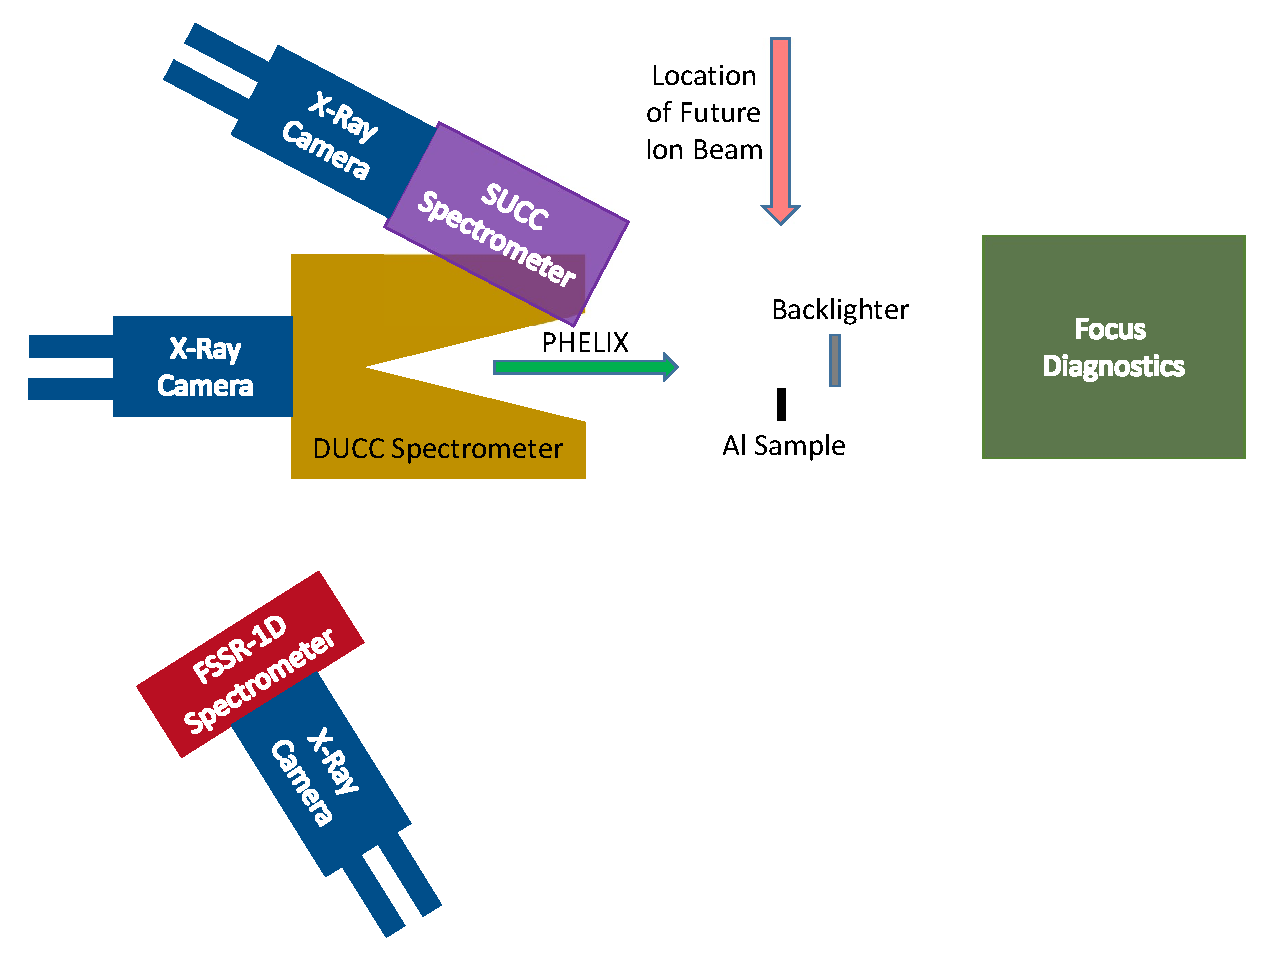
\includegraphics[width = 0.79\textwidth]{Diagrams/Experimental_setup_schematic.pdf}
	\caption{Schematic illustration of the experimental setup. Note that the 
	location of the heavy-ion beam for future experiments is marked, but of 
	course not present in this experiment. The DUCC and SUCC spectrometers are 
	not in the plane of the illustration, but tilted downwards and upwards 
	respectively. At any one time there are only two cameras in the setup. The x-ray cameras can be freely transferred between the 
	spectrometers.}
	\label{fig: setup schematic}
\end{figure}

\begin{figure}[H]
	\centering
	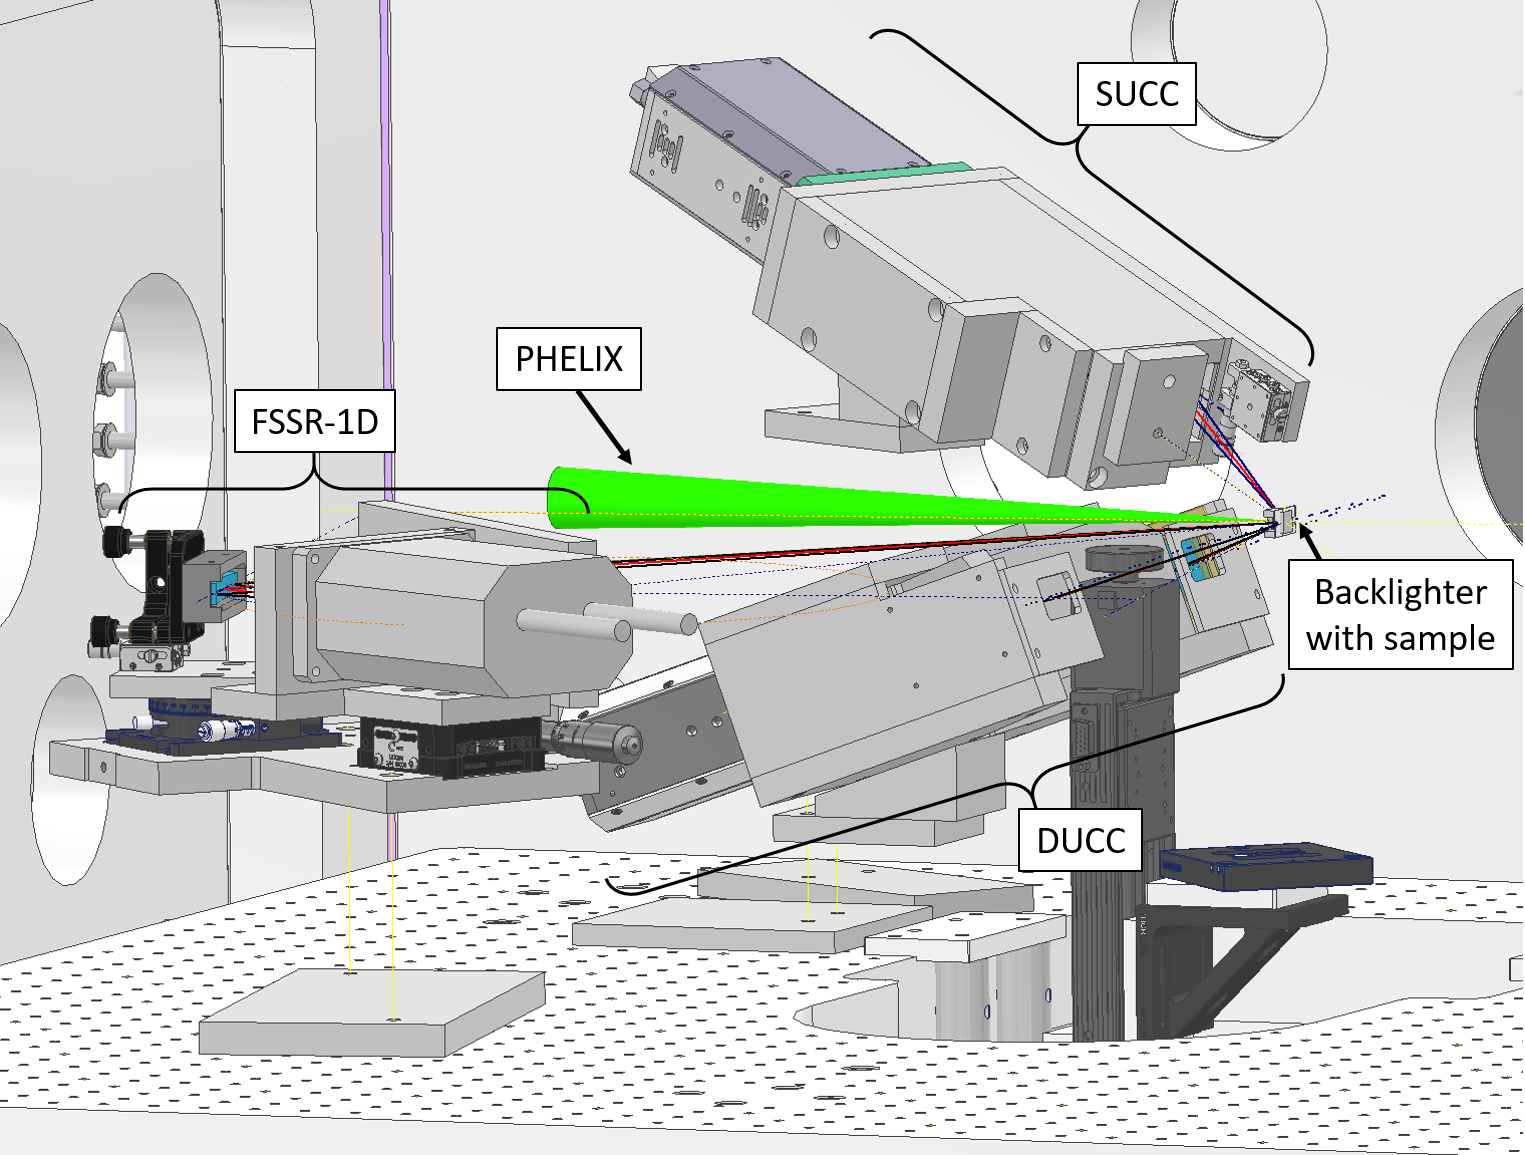
\includegraphics[width = 0.7\textwidth]{Diagrams/Inv_HHT_labeled.PNG}
	\caption{\textit{Inventor} model of the HHT chamber from the perspective of 
	the 
	bottom right of fig. \ref{fig: setup schematic} looking towards the 
	spectrometers. The heavy-ion beam as well as the focus diagnostics are not 
	pictured. The optical posts that connect the spectrometers to their bases 
	are not shown, but their locations are depicted with thin yellow lines. 
	Additionally, the optical paths in the dispersive direction for each 
	spectrometer are shown in blue, with a red line for the central rays. In 
	actuality the PHELIX beam extends out of the chamber.}
	\label{fig: setup inventor}
\end{figure}

\section{Mechanical Design of Spectrometers}
\label{section: mechanical design}

I based the mechanical design of the spectrometers around four goals. First, 
the devices must implement the designs presented in chapter \ref{chapter: 
spectrometer design} to an approximately $\pm$\SI{0.5}{\milli\meter} precision, 
ensuring that sufficient internal and external alignment to produce 
well-resolved spectra is achieved. Second, the crystal and camera chip must be 
sufficiently shielded while still maintaining enough intensity on the detector. 
Third, alignment of the spectrometer components to one another and the 
backlighter must be addressed. This requirement is more stringent for the 
FSSR-1D as a consequence of its focusing properties. Finally, the devices must 
be robust enough to withstand the harsh experimental conditions resulting from 
the heavy-ion beam and plasma. This mainly takes the form of heavy aluminum 
shielding, among others.

In this section, I will describe the 
mechanical designs of the DUCC and FSSR-1D, whose models are built in the CAD 
program \textit{Autodesk Inventor 2020}. The SUCC will not be elaborated on, as 
it is not designed by me and generally shares a similar mechanical design 
philosophy with a single channel of the DUCC. All spectrometers are 
outfitted with in-vacuum 
CCD cameras from \textit{greateyes} of the GE-VAC 2048 512 
series as detectors. In the case of the DUCC, an adjusted camera 
with a thinner front plate is used to avoid clipping. The 
spectrometer parts are generally made of aluminum, unless otherwise 
specified.


\subsection{Dual Unbent Crystal Spectrometer}

The DUCC model is shown in fig. \ref{InvDUCC} with the parts 
color 
coded, which is presented in table \ref{Table: DUCC colors}, 
along with 
a summary of their functions and names. The 
most numerous parts are the ones responsible for shielding and 
structure. These protect the chip and crystals from debris, 
particles 
and extraneous rays. Also serving a shielding role is a pointer 
holder, 
whose main purpose is to hold the optical post for alignment 
purposes.

\begin{table}[H]
	\centering
	\caption{Color code of the DUCC model with the functions and name 
		of 
		the parts.}
	\vspace{0.05cm}
	\renewcommand{\arraystretch}{1.5}
	\centering
	\begin{tabular}{|c|c|c|} 
		\hline
		Color & Function & Name \\ [0.5ex]
		\hline\hline
		Light gray & Structural/Shielding & - \\ 
		[0.5ex]
		\hline
		White (near source) & Protecting crystal & Blast shield \\ 
		[0.5ex]
		\hline
		White (labeled) & Capturing spectra & Greateyes camera\\ 
		[0.5ex]
		\hline
		Brown & Capturing spectra & Camera chip \\ 
		[0.5ex]
		\hline
		Dark gray & Holding alignment post & Pointer holder \\ 
		[0.5ex]
		\hline
		Red (front of camera) & Separating spectra/holding filter & 
		Filter holder \\ [0.5ex]
		\hline
		Transparent yellow & Securing crystals & Crystal frame \\ 
		[0.5ex]
		\hline
		Turquoise & Dispersion of rays & ADP crystal \\ [0.5ex]
		\hline
		Green & Supporting + tilting spectrometer & Foot with angled 
		block \\ 
		[0.5ex]
		\hline
		Beige & Display location of chamber floor & Breadboard floor \\ 
		[0.5ex]
		\hline
		Red & - & Central ray \\ 
		[0.5ex]
		\hline
		Black & - & Outer rays \\ [0.5ex]
		\hline
	\end{tabular}
	\label{Table: DUCC colors}
\end{table}

The blast shields, on which \SI{2}{\micro\meter} Mylar foils are 
attached to the opening, protect the crystal from debris while 
allowing 
the x-rays through. Additionally, two carbon filters are glued 
onto the 
openings of the filter holder, which are light-tight and prevent 
visible light from reaching the chip. These carbon 
filters can be chosen to have an areal density of 
$\approx\SI{200}{\micro\gram\per\cm\squared}$ or 
$\approx\SI{900}{\micro\gram\per\cm\squared}$, depending on the 
intensities observed on the chips in the experiment. The filter 
holder 
also 
serves to spatially separate the two channels 
onto the chip, where the holes have a vertical separation of 
\SI{1}{\milli\meter} so that a shadow will appear on the center 
line of 
the chip.

The ADP crystals are held in place by first placing them in a 
groove, 
then screwing on the crystal frames made of Trovidur. By 
attaching a 
plexiglass foil to the bottom of the groove and fabricating the 
frames 
out of plastic, the crystal is protected from direct contact with 
the 
aluminum housing. The $20\degree$ angle of the DUCC w.r.t. the 
PHELIX 
beam is implemented by an angled block of the foot. Finally, a 
venting 
channel is engraved into the plate attached to the camera, 
partially 
visible in fig. \ref{InvDUCCFullBack}. This channel is designed 
with 
random turns, similar to a snake, so that air can escape while 
light is 
kept out. This is essential to prevent the carbon filters from 
breaking 
during venting of the HHT chamber.


The alignment is realized by first affixing the pointer holder 
with 
screws to 
the top and bottom plates of the shielding, making sure to use 
the 
groove on 
the bottom plate to guarantee proper orientation. Then an optical 
post 
is set 
to the designed distance from the front surface of the pointer 
holder 
to the 
x-ray source. The post is attached to the pointer holder and the 
DUCC 
is brought into 
the chamber. Once the tip of the post is as close as possible to 
the 
laser-target interaction point, known as the target chamber 
center 
(TCC), the spectrometer is aligned, as the alignment of 
further degrees of freedom
is guaranteed by the mechanical precision of the structural 
pieces, reaching the desired precision of $\pm$\SI{0.5}{\milli\meter}.

\begin{figure} [H]
	\centering
	\begin{subfigure}[t]{0.34\textwidth}
		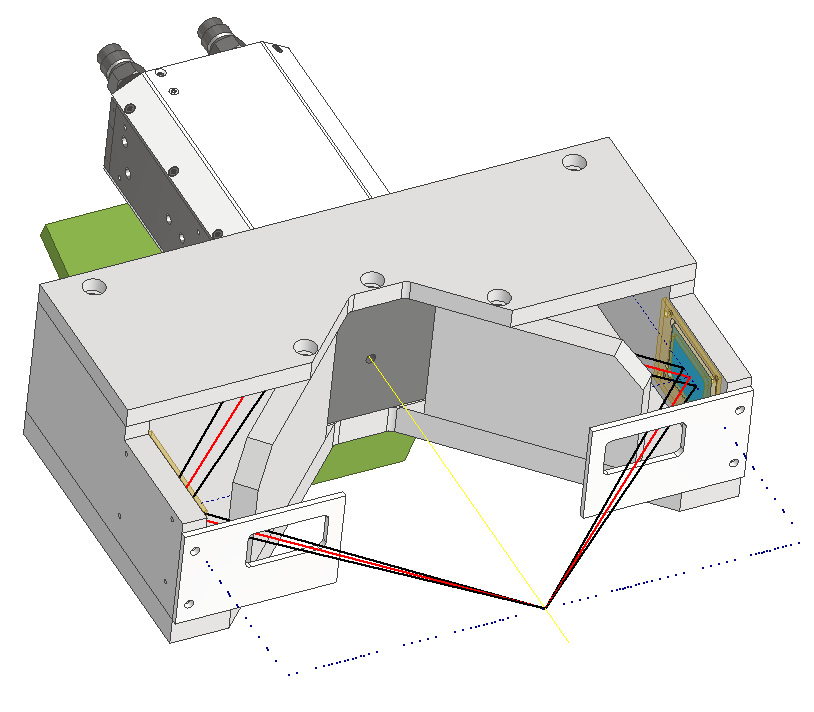
\includegraphics[width=\textwidth]{InventorPics/FullDUCC.PNG}
		\caption{Front view.}
		\label{InvDUCCFullFront}
	\end{subfigure}%
	\hfill
	\begin{subfigure}[t]{0.64\textwidth}
	\centering
		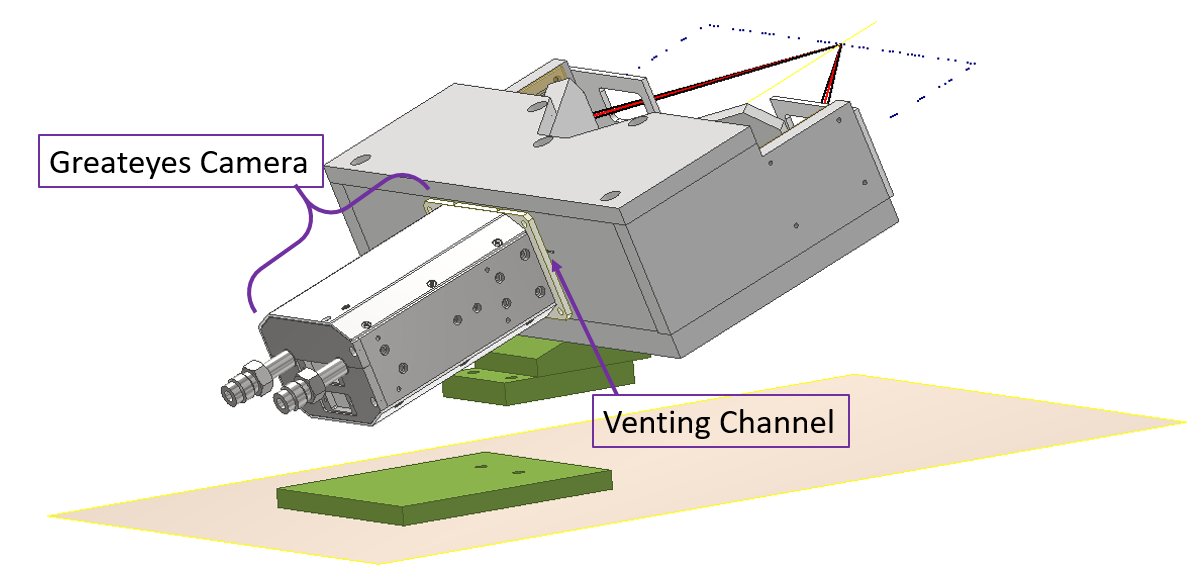
\includegraphics[width=\textwidth]{InventorPics/FullDUCCBack.PNG}
		\caption{Back view with Greateyes camera and venting 
		channel 
		labeled.}
		\label{InvDUCCFullBack}
	\end{subfigure}\\[1ex]
	\centering
	\begin{subfigure}[t]{0.35\textwidth}
		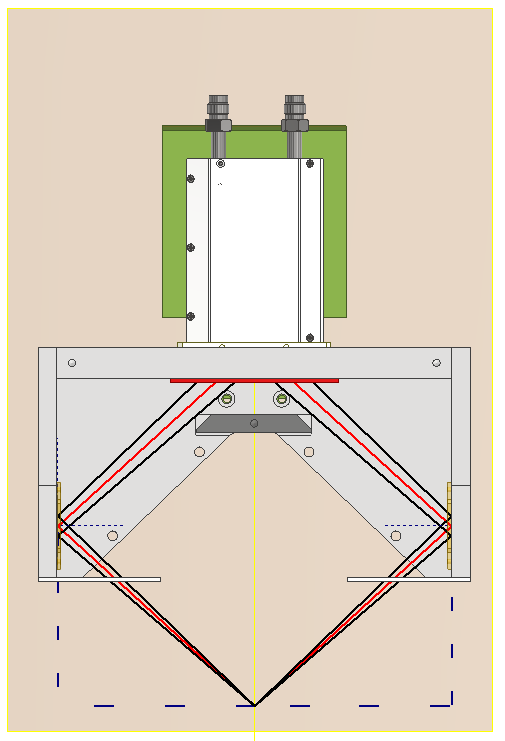
\includegraphics[width=\textwidth]{InventorPics/DUCCTopWoCover.PNG}
		\caption{Top view with top and inner shielding hidden.}
		\label{InvDUCCPartTop}
	\end{subfigure}%
	\hfill
	\begin{subfigure}[t]{0.63\textwidth}
	\centering
		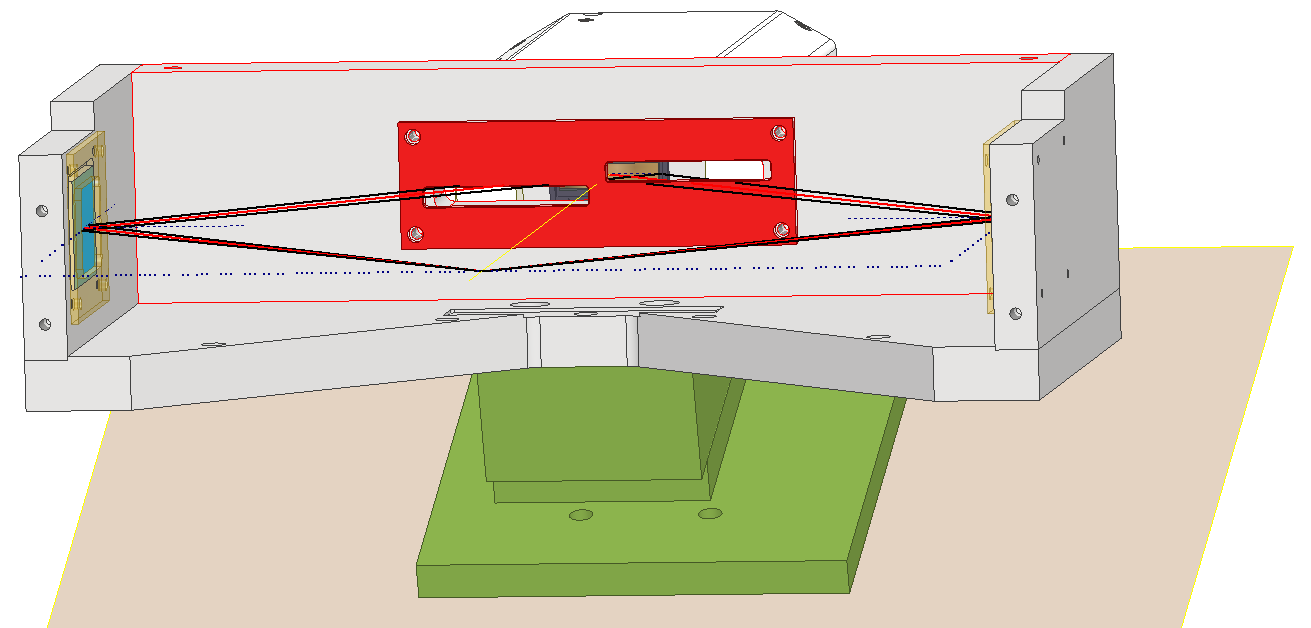
\includegraphics[width=\textwidth]{InventorPics/DUCCFilterView.PNG}
		\caption{Front view with top and inner shielding as well 
		as the pointer 
		holder hidden.}
		\label{InvDUCCPartFilter}
	\end{subfigure}
	\caption{CAD model of the DUCC. The parts are color coded, 
	whose 
	function and name are listed in table \ref{Table: DUCC 
	colors}.
	The optical posts between the foot parts are not depicted.}
	\label{InvDUCC}
\end{figure}

\begin{figure} [H]
	\centering
	\begin{subfigure}[t]{0.45\textwidth}
		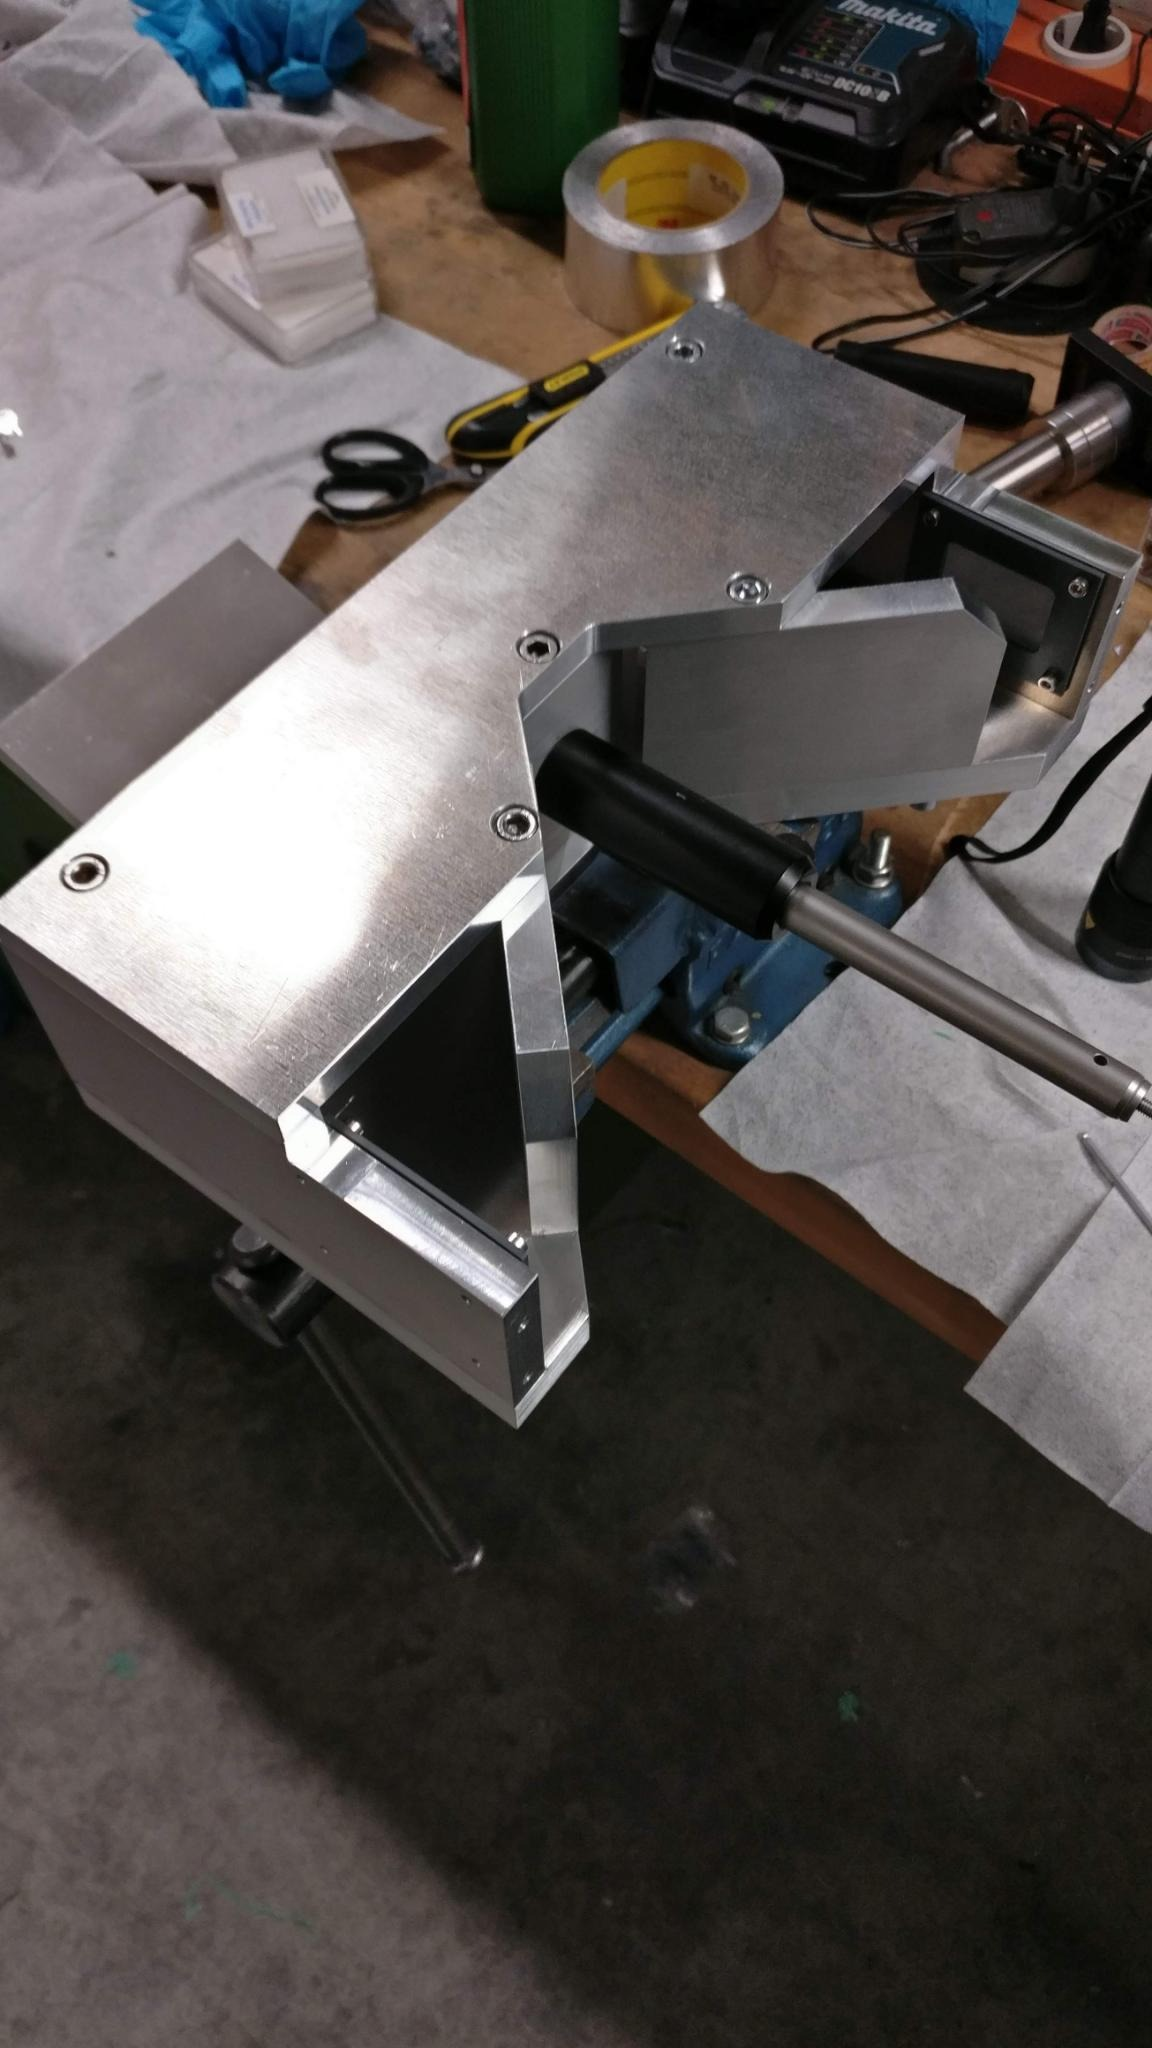
\includegraphics[width=\textwidth]{InventorPics/Real_pic_DUCC_complete.jpeg}
		\caption{Top view.}
	\end{subfigure}%
	\hfill
	\begin{subfigure}[t]{0.45\textwidth}
		\centering
		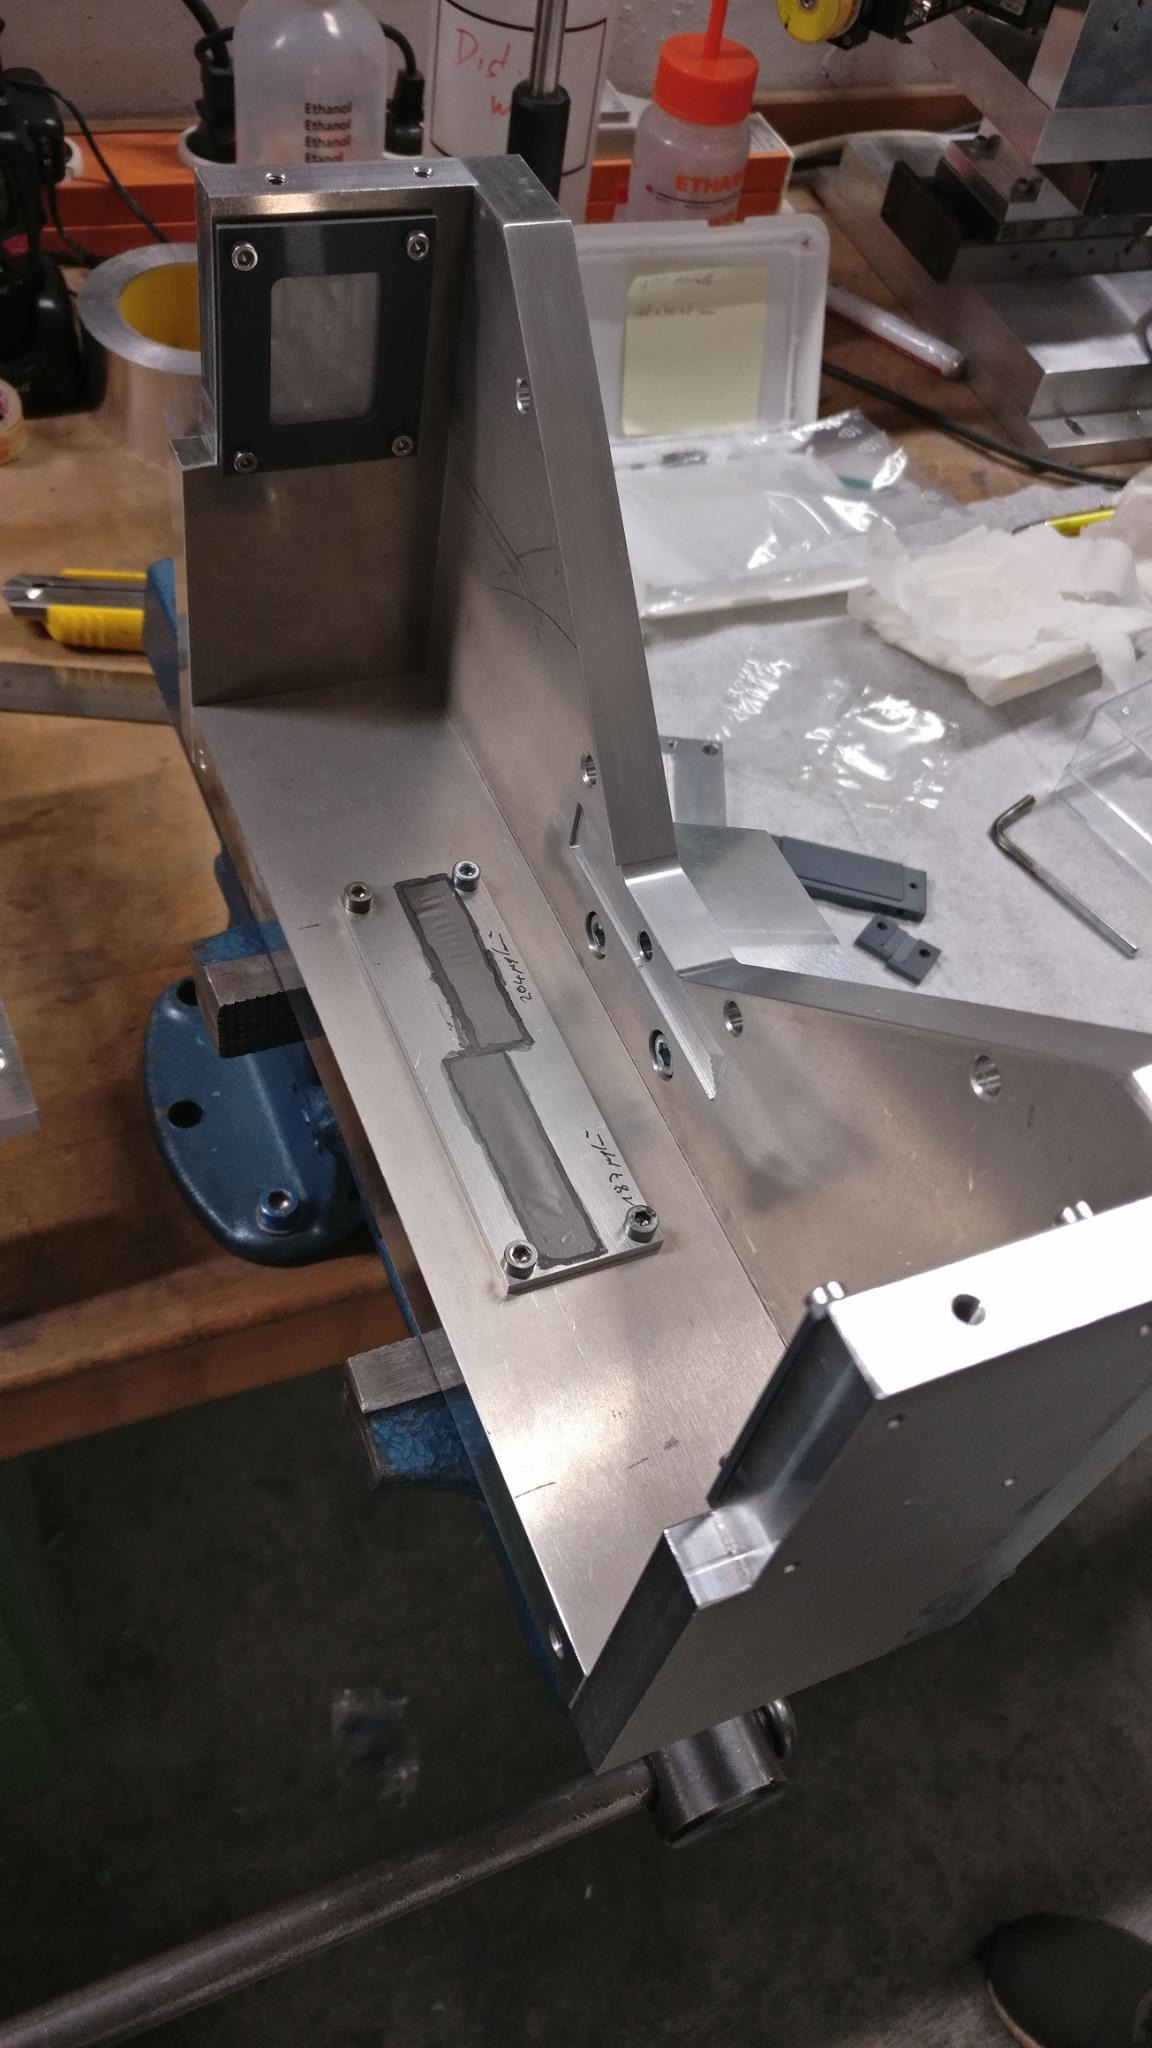
\includegraphics[width=\textwidth]{InventorPics/Real_pic_DUCC_inside.jpeg}
		\caption{Inside view.}
	\end{subfigure}\\[1ex]
	\caption{Pictures of the DUCC before the experiment without the camera.}
\end{figure}

\subsection{Focusing Spectrograph with Spatial Resolution}

In fig. \ref{InvFSSR} the FSSR-1D model is pictured with the 
parts 
color coded, presented in table \ref{Table: FSSR colors} with 
a summary of their functions and names. The shielding in this 
setup is mainly taken care of by the front plate closest to TCC. 
A 
snout, formed by three plates, adds additional shielding in 
front of the chip, as well as functioning as an aperture at the 
polychromatic crossover as described in section 
\ref{SectionTheoryFSSR}. Inside the 
snout is the carbon filter 
holder, which fulfills the same role as with the DUCC, except 
this time 
using only the $\approx\SI{900}{\micro\gram\per\cm\squared}$ 
carbon 
filter. Additionally, a blast shield is attached to the front 
plate, 
set up the same way as in the DUCC. The crystal itself was originally planned 
to be fixed 
by the 
crystal holder, designed in such a way that the reflecting 
surface does 
not come into contact with anything. In the experiment, this holder couldn't be 
used, as the mica crystal was a different one than planned, namely one that 
came in its own holder. 

\begin{table}[H]
	\centering
	\caption{Color code of the FSSR-1D model with the functions and 
		name of 
		the parts. Note that there are four optical stages which are not 
		color 
		coded. These are used in the alignment process, so are labeled in 
		fig. 
		\ref{InvFSSRAlignment}.}
	\vspace{0.05cm}
	\renewcommand{\arraystretch}{1.5}
	\centering
	\begin{tabular}{|c|c|c|} 
		\hline
		Color & Function & Name \\ [0.5ex]
		\hline\hline
		Light gray & Structural/Shielding & - \\ 
		[0.5ex]
		\hline
		Light gray (labeled) & Capturing spectra & Greateyes camera \\ 
		[0.5ex]
		\hline
		Brown & Capturing spectra & Camera chip \\ 
		[0.5ex]
		\hline
		White & Aperture at crossover/Shielding & Snout \\ 
		[0.5ex]
		\hline
		Dark gray & Securing crystal & Crystal holder \\ 
		[0.5ex]
		\hline
		Red (front of camera) & Holding carbon filter & 
		Filter holder \\ [0.5ex]
		\hline
		Dark blue & Protecting crystal & Blast shield \\ 
		[0.5ex]
		\hline
		Turquoise & Dispersion of rays & Mica crystal \\ [0.5ex]
		\hline
		Green & Support & Foot \\ 
		[0.5ex]
		\hline
		Beige & Display location of chamber floor & Breadboard floor \\ 
		[0.5ex]
		\hline
		Red & - & Central ray \\ 
		[0.5ex]
		\hline
		Black & - & Outer rays \\ [0.5ex]
		\hline
		Olive green & - & Highest energy ray \\ [0.5ex]
		\hline
	\end{tabular}
	\label{Table: FSSR colors}
\end{table}

Shown in fig. \ref{InvFSSR} are also optical stages utilized 
for the 
alignment procedure, which 
must be more exacting than that of the DUCC, owing to the 
curvature of the 
crystal and therefore the imaging and focusing properties. 
As the 
alignment is 
an involved process using additional components not pictured 
in fig. 
\ref{InvFSSR}, it is described in detail in the appendix, section 
\ref{section: 
	FSSR-1D alignment}.

The precision of the internal alignment of $\pm$\SI{0.5}{\milli\meter} is 
realized with a series of grooves, where each part attached to the main plate 
is set into a groove. The alignment process use the various optical stages 
further guarantees the desired precision.


\begin{figure} [H]
	\centering
	\begin{subfigure}[t]{0.42\textwidth}
		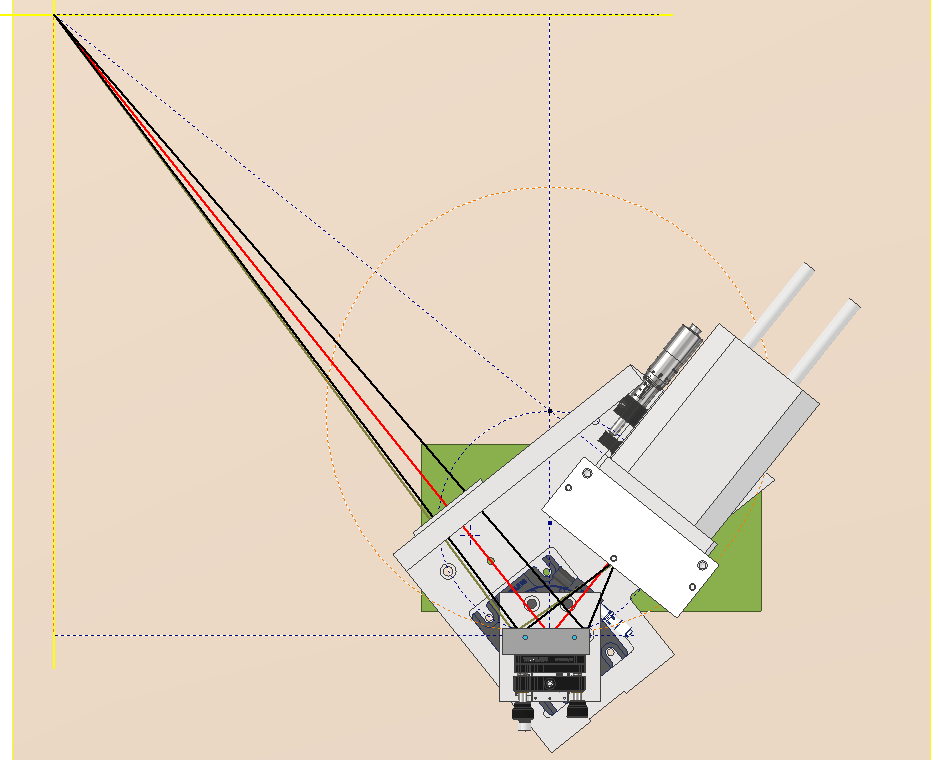
\includegraphics[width=\textwidth]{InventorPics/FSSRFullTop.PNG}
		\caption{Top view.}
		\label{InvFSSRFullTop}
	\end{subfigure}%
	\hfill
	\begin{subfigure}[t]{0.56\textwidth}
	\centering
		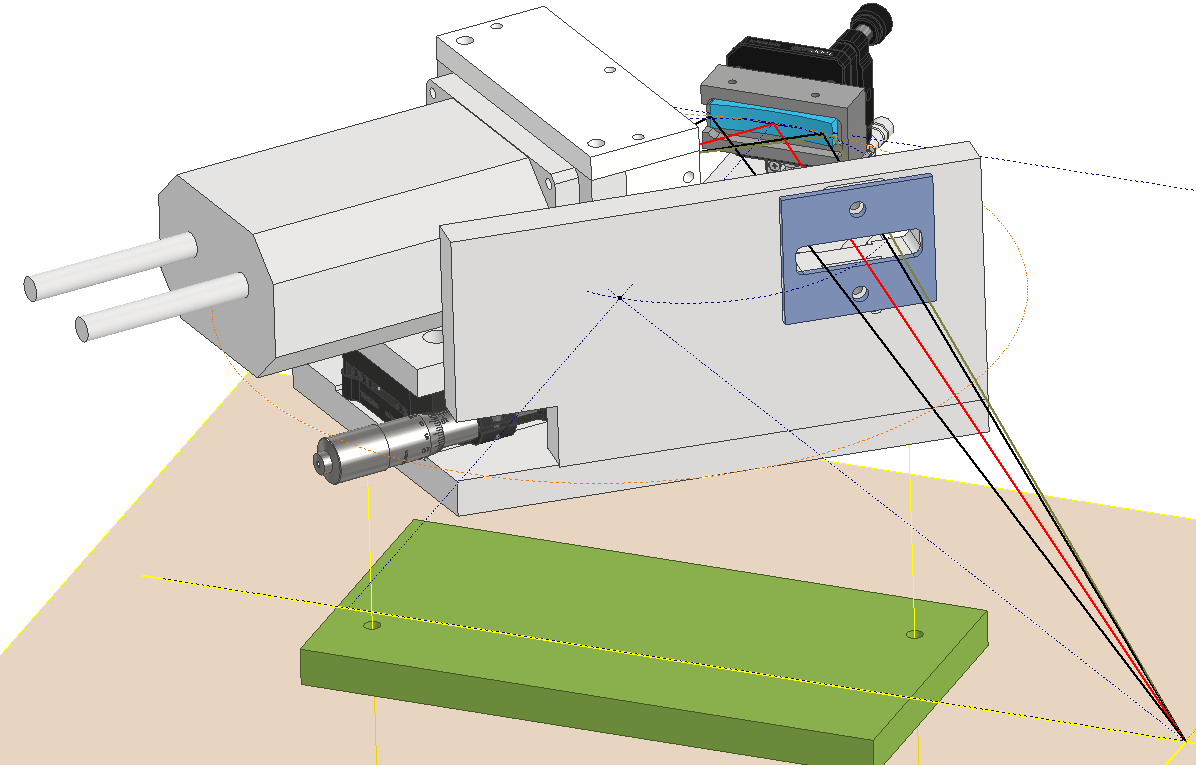
\includegraphics[width=\textwidth]{InventorPics/FSSRFullFront.PNG}
		\caption{Front view.}
		\label{InvFSSRFullFront}
	\end{subfigure}\\[1ex]
	\centering
	\begin{subfigure}[t]{0.6\textwidth}
	\centering
		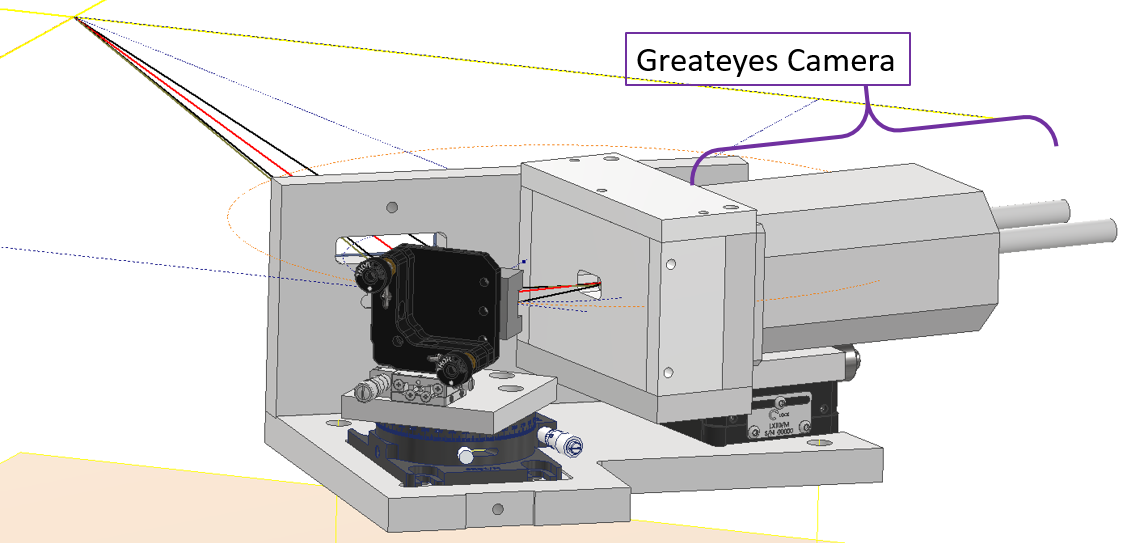
\includegraphics[width=\textwidth]{InventorPics/FSSRFullBack.PNG}
		\caption{Back view with Greateyes camera labeled.}
		\label{InvFSSRFullBack}
	\end{subfigure}%
	\begin{subfigure}[t]{0.38\textwidth}
	\centering
		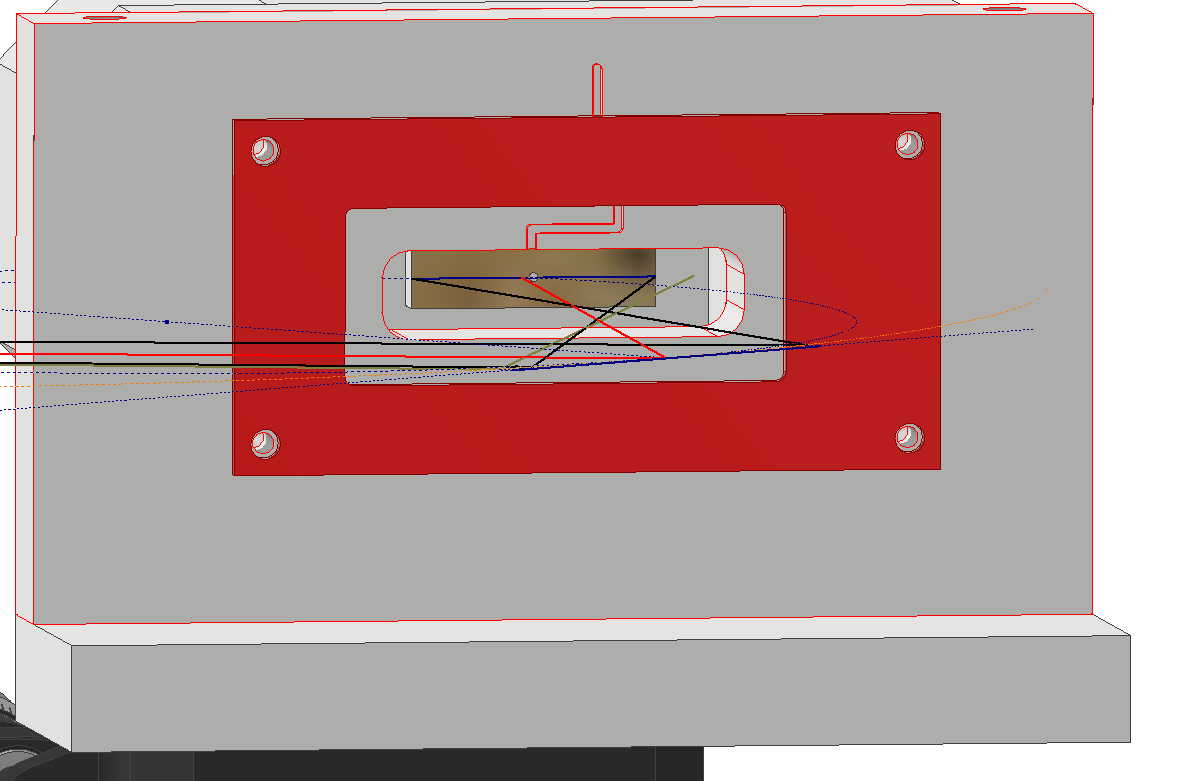
\includegraphics[width=\textwidth]{InventorPics/FSSRCameraNoSnout.PNG}
		\caption{View onto chip with snout and camera apparatus 
		hidden. 
		Venting channel is shown behind the filter holder.}
		\label{InvFSSRPartCamera}
	\end{subfigure}
	\caption{CAD model of the FSSR-1D. The parts are color coded, 
	whose 
	function and name are listed in table \ref{Table: FSSR 
	colors}. 
	Note that the optical posts between foot and bottom plate are 
	not 
	shown. The various optical stages for aligning the 
	spectrometer are 
	shown, but not color coded.}
	\label{InvFSSR}
\end{figure}

\begin{figure}[H]
	\centering
	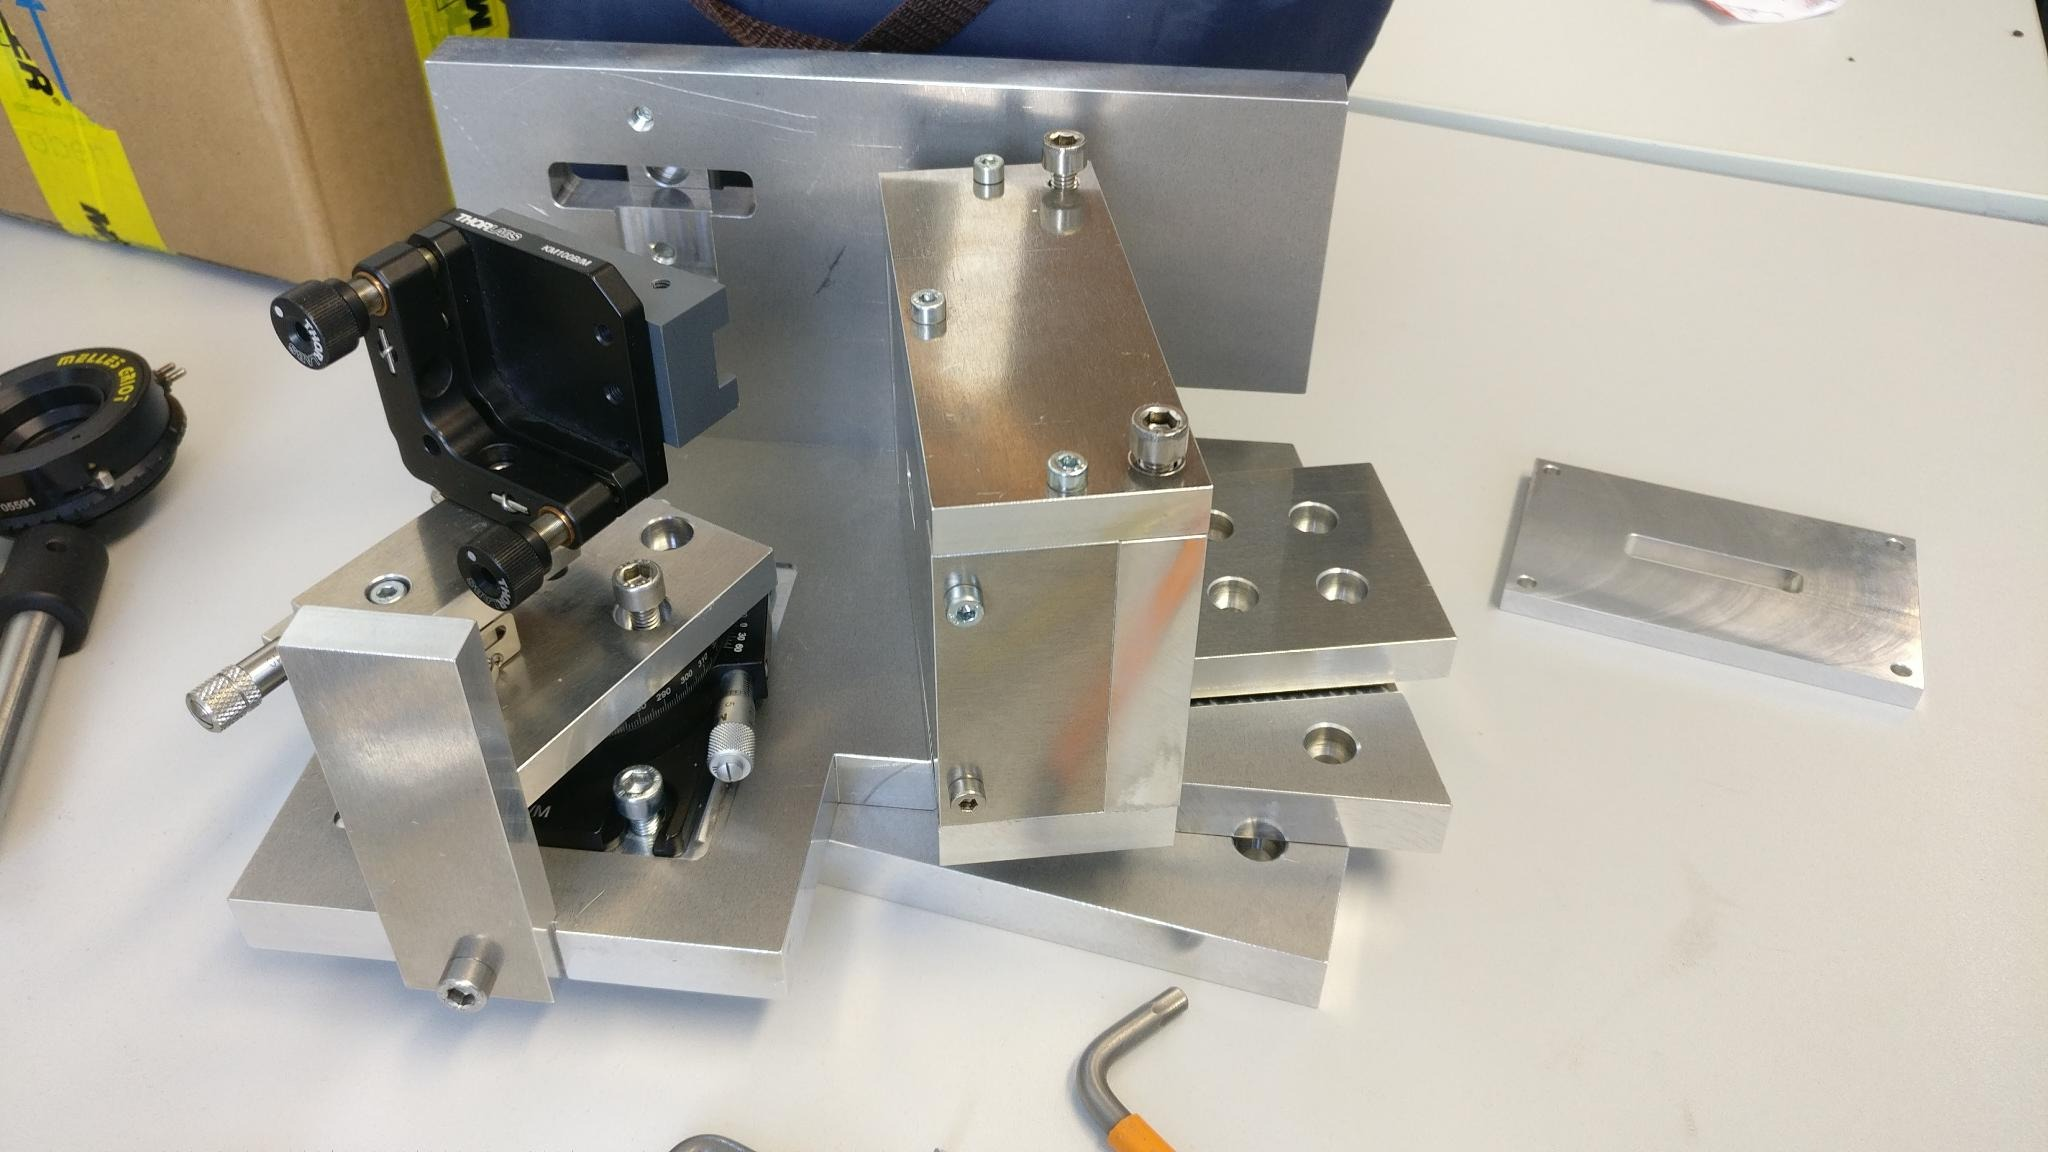
\includegraphics[width = 0.95\textwidth]{InventorPics/Real_pic_FSSR.jpeg}
	\caption{Picture of the FSSR before the experiment without the camera.}
\end{figure}





	\chapter{Data Analysis}
\label{chapter: data analysis}

In this chapter, I will describe the analysis of the data collected in the laser-only experiment conducted in May 2023, with a focus on the spectrometers and their ability to produce spectra capable of high-resolution XAFS. I will start by explaining the processing of the raw images from the cameras into spectra, then I will outline the results to be derived from them. 

I carry out the analysis with a program that I developed in 
\textit{python3} called \textit{AXAWOTLS}, which stands for "Analysis of X-ray Absorption for WDM Observation and Testing of Locally-made Spectrometers". It is capable of reading a 
TIFF image and outputting fully processed spectra, as well as performing further analysis with these spectra. The code is designed from the 
ground up to be applicable to any x-ray spectrometer intended for XAFS and allow "online" data analysis 
during a beamtime, producing results for any given event in less than a few 
minutes. With this processing speed and its ease-of-use, requiring only that the user input parameters, it is my hope that this code lets future researchers involved in WDM 
research with XAFS at PHELIX effectively interpret and act on raw data in a 
beamtime, simplifying the workflow. 

The code consists of two main parts. The first is responsible for producing 
workable spectra from raw TIFF images, while the second encompasses further processing and application of these spectra for 
data analysis.
The general workflow of the code to produce a spectrum is illustrated 
in fig. \ref{fig: analysis overview}. First, horizontal line outs of each 
spectrum in the TIFF image are taken by selecting the corresponding area in the 
image and averaging over the pixels in the vertical direction. This yields the 
counts for each pixel, which are numbered starting from the leftmost edge of 
the image. Next, spectra are flipped depending on the orientation of the camera 
chip and spectrometer channels. The background is subtracted and the 
pixel number is converted to photon energy according to the dispersion of the 
spectrometer. To note is that this dispersion must be first calibrated by a 
previously known emission line, in this work the Al He-$\upalpha$ line.

At this 
point the second part of the code, the data analysis, takes over, further processing the spectra as follows. First, the filters on the spectrometers are corrected out using the transmission 
values from the CXRO database of Berkeley Lab \citep{cxro_database}. Then, the corrected counts $N_{\text{counts}}$ are converted to photon number on detector $N_{\text{det}}$ with the formula
\begin{equation}
N_{\text{det}} = \frac{N_{\text{counts}}\cdot E_{\text{hole}}}{G\cdot E_{\text{ph}}\cdot Qe},
\label{eq: detector correction}
\end{equation}
where the 
gain $G$, energy needed to generate a photoelectron-hole pair $E_{\text{hole}}$, and quantum 
efficiency $Qe$ are all properties of the x-ray camera found in its 
specification sheet. Next, the number of photons emitted by the source per steradian and energy interval $N_{\text{st,eV}}$ is estimated with the equation
\begin{equation}
	N_{\text{st,eV}} = \frac{N_{\text{total}}}{4\pi \Delta E} = \frac{N_{\text{det}}\cdot D}{\Delta x_{\text{pix}}\cdot R_{int}\cdot \Delta E},
	\label{conversion to emitted photons}
\end{equation}
adapted from Döppner \textit{et al.} \citep{doppner2008high}, where $N_{\text{total}}$ represents the total number of photons emitted by 
the source, $D$ 
the distance 
over which the x-rays diverge (for example, the optical path length 
from source 
to detector for flat crystal geometries), $\Delta x_{\text{pix}}$ the 
pixel width in the non-dispersive direction (i.e. the physical length which collects the rays), and $\Delta E$ the energy interval covered by a pixel. Notably, $\Delta E$ is assumed to be constant, as the dispersion of the spectrometers is approximately linear, and the integrated reflectivity $R_{int}$ is taken from the literature, as it is not directly measurable in this experiment. Finally, the spectra can be smoothed through binning over eight pixels, i.e. eight data points.

It is also important to note that the processing is slightly different for the FSSR, where it is summed instead of averaged over the pixel rows of the spectrum to get a horizontal line out. This is due to the imaging properties of the geometry in the non-dispersive direction, as the x-rays only diverge until reaching the crystal, where they are then imaged onto the detector. Accordingly, one must sum the contributions in the non-dispersive direction to accurately represent the signal. As a consequence of the summing, the background is estimated by first averaging to get a horizontal line out, then multiplying by the number of pixel rows summed over for the signal spectrum. As the photons on the camera chip are collected by the entire width of the mica crystal, the diverging distance $D$ and the collecting length $\Delta x_{\text{pix}}$ in formula \ref{conversion to emitted photons} must be adjusted so that $\Delta x_{\text{pix}} \longrightarrow w_{\text{crystal}}$, where $w_{\text{crystal}}$ represents the crystal width in non-dispersive direction, and $D$ becomes the source-crystal distance $a_0$. Otherwise, the spectrum extraction is analogous to the flat crystal geometries.

For finer details of the calculations, please refer to the source code of \textit{AXAWOTLS}, which can be requested by sending me an email at carlosbutler210@gmail.com.

\begin{figure}[H]
	\centering
	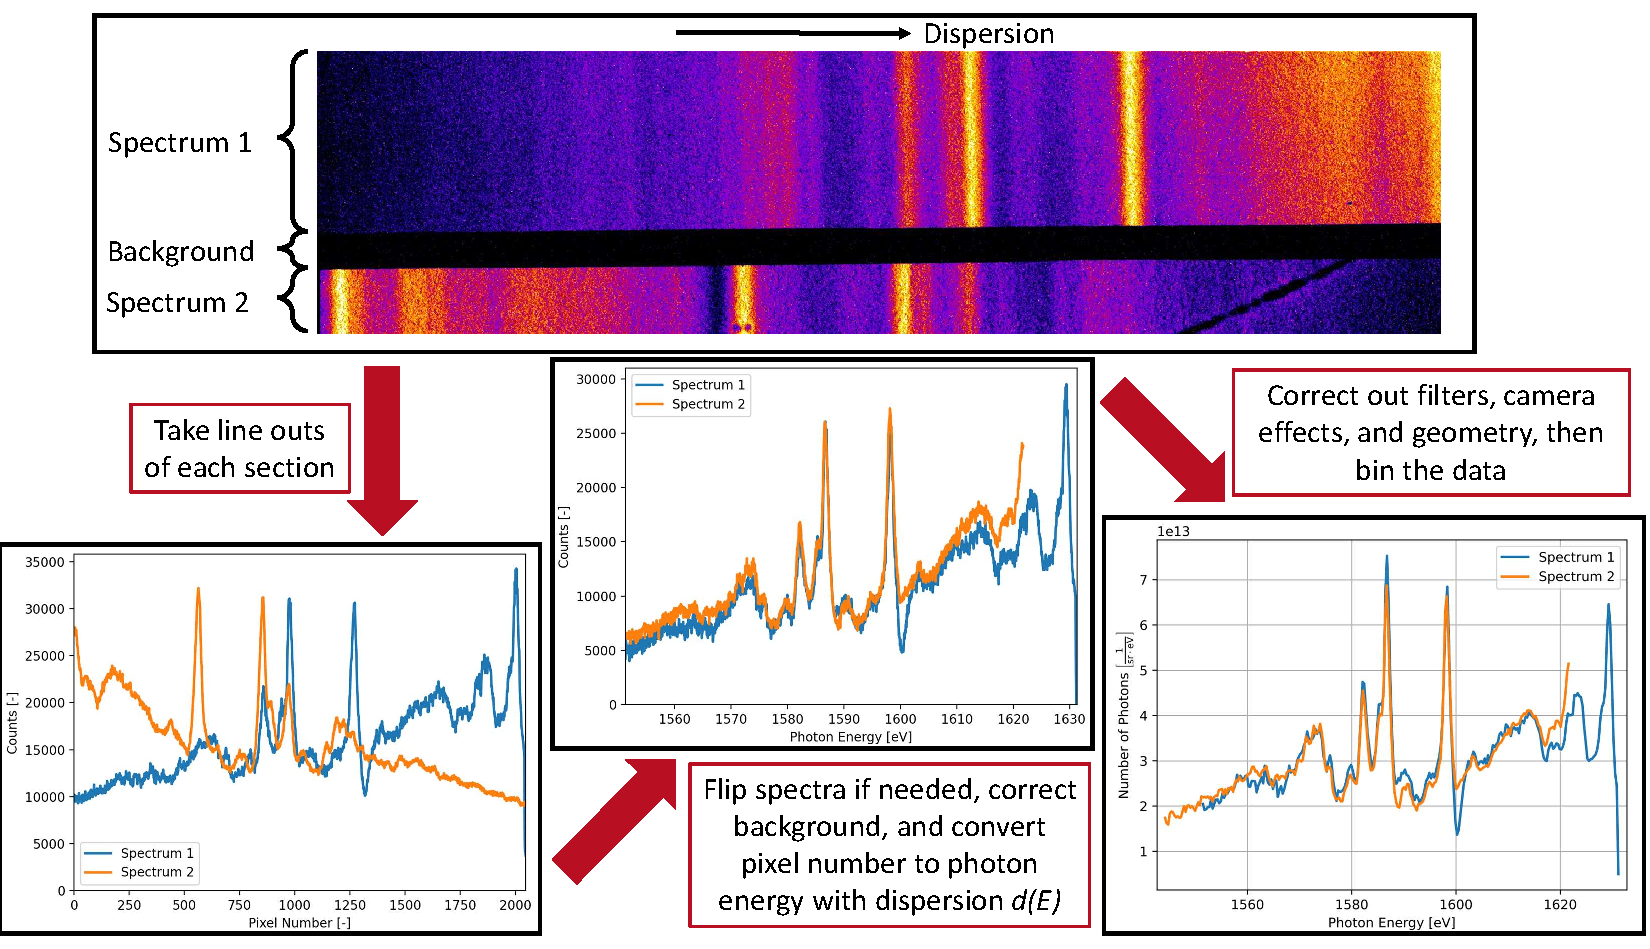
\includegraphics[width=\textwidth]{Data_Analysis/Analysis_overview.pdf}
	\caption{Overview of the data analysis steps from raw TIFF image to fully 
	processed spectrum. Example is of spectra from a Dy plasma ignited with a 
	\SI{57.3}{\joule} laser pulse, recorded with the DUCC. In the raw image, 
	the higher the count, the warmer the color, so yellow represents the maxima 
	and dark purple towards black the minima.}
	\label{fig: analysis overview}
\end{figure}



	\chapter{Results and Discussion}
\label{chapter: results and discussion}

In this chapter, I will present and discuss the results gained from spectra produced and analyzed by the self-developed code \textit{AXAWOTLS}. I will organize the results into three categories:

\begin{enumerate}
	\item \textbf{Qualitative Performance:} The results in this category serve to 
	assess the spectrometers qualitatively and to touch on the properties 
	of the laser-driven backlighters. The fundamental 
	outputs of the spectrometers will be presented, which take the form of source 
	spectra of various backlighter targets as well as absorption spectra of cold 
	aluminum, where here cold refers to ambient vacuum temperatures.
	\item \textbf{Spectrometer Characterization:} This covers the quantitative characterization of the spectrometers, consisting of the calculation of the spectral resolution through two spectral 
	features: the He-$\upalpha$ line (corresponding to the n=2 to n=1 transition of 
	He-like ions, starting from 2p$^1$P$_1$) of aluminum in source spectra 
	and the Al 
	K-edge in transmission spectra. Additionally, the ratio of integrated 
	reflectivities of both spectrometers for a given event will be determined. To note is that the 
	integrated reflectivity itself cannot be directly determined, as the total 
	emission of the x-ray sources are unknown.
	\item \textbf{Setup Validation:} The purpose of this category is to check that 
	the experimental setup yields plausible results considering the characteristics of the x-ray sources. To this end the conversion efficiency 
	of the laser energy into the Al He-$\upalpha$ emission is determined, serving as a quantitative validation through comparison to literature.
\end{enumerate}

In light of the results, the effectiveness of each spectrometer design in the context of this work will be discussed. I will then use these considerations to inform a recommended spectrometer design for future experiments.

I will begin with the qualitative performance, which will be 
prefaced by a brief introduction to the main mechanisms of X-ray emission from laser-generated plasmas, since 
it is important for the discussion of the source and absorption spectra. This 
will be followed by the spectrometer characterization and setup validation. For each set of results, I will first explain the processing steps, then present the results, and end with a discussion detailing the ramifications for the spectrometer designs. In addition, the error calculations will be described in the appendix chapter \ref{chapter: uncertainty analysis}.

\section{Qualitative Performance}
\label{section: qualitative performance}

As stated in the spectrometer comparison of section \ref{section: specs and comparison}, neither the DUCC nor the FSSR-1D clearly distinguishes itself from design specifications, e.g. in terms of theoretical relative resolution and sample size. As such, the qualitative assessment of the performance of each spectrometer during the experiment plays an important role. The most significant results in this area are of course the absorption spectra, whose quality depends on a number of experimental factors and mechanical properties, e.g. crystal quality, backlighter type, accuracy of the alignment of the setup, etc. To understand the details of the XAFS spectra quality, it is necessary to first study the spectra of the x-ray sources, i.e. the laser-driven plasma emission. Accordingly, I will begin by summarizing the main x-ray emission mechanisms in laser-driven plasma, then present source spectra.


\subsection{X-ray Source Spectra}

There are three main mechanisms responsible for
x-ray emission in laser-generated plasma, each identifiable by their characteristics on the spectrum \citep{riley2021warm, 
	giulietti1998x}. The first originates from scattering of free electrons with 
ions in the plasma. This generates bremsstrahlung and 
gives a smooth emission spectrum, where the intensity
decreases for increasing photon energy. As this 
emission depends on average ionization, it is 
strongest for high Z materials. The second is 
recombination, in which free electrons recombine with 
ions and radiate a photon. This also results in a 
continuous spectrum, but deviates from bremsstrahlung emission in that it occurs from a minimum photon energy 
called the recombination edge. These edges also 
result in jumps in the spectrum corresponding to 
recombination stages. The third is line emission, 
occurring for transitions of bound electrons between 
states. This is the strongest source of x-ray 
radiation in terms of photons per energy interval, but is also discrete \citep{giulietti1998x}. 

Based on these different kinds of x-ray emission mechanisms, the characteristics of x-ray backlighters can be tailored to their application. An ideal x-ray source for XAFS would exhibit a high-intensity, spectrally quasi-continuous spectrum, as this reduces the chance of spectral structure, like peaks or edges, impacting the absorption spectrum, as well as ensures good signal-to-noise ratios \citep{riley2021warm, eason1984improved}. In practice, continuum x-ray emission is usually realized by plasma of either very low-Z or high-Z ($\geq$20) material. In the case of very low-Z targets, ions are fully stripped, thus suppressing line emission so that Bremsstrahlung dominates. For high-Z targets, the spectrum is dominated by line emissions from many-electron interactions, leading to a high line density and therefore a quasi-continuous spectrum. As such, very low-Z targets offer smooth spectra at the cost of having low intensity, while high-Z backlighters yield high intensities with potential significant structure in the spectrum \citep{giulietti1998x}.

In light of this, five high-Z elements are tested in this experiment, namely gold and four rare earth elements: samarium, 
gadolinium, terbium, and dysprosium. Additionally, a low-Z material is investigated in the form of Teflon. Figure \ref{figure: basic spectra} depicts source spectra for each backlighter material as well as aluminum, a material used for spectrometer characterization and as a control. The spectra are all extracted and processed according to the procedure described in chapter \ref{chapter: data analysis}. When available, events with different laser energies are shown. All the source spectra, excepting those of Teflon, are captured with the DUCC, as it simultaneously displays the fewest spectral artefacts, often originating from crystal defects or damage, and good resolution, as will be demonstrated in section \ref{subsection: spectral resolution}. Owing to the lower intensity of the emission as compared to the high-Z elements, the Teflon source spectra are taken with the SUCC, whose KAP crystal has a higher integrated reflectivity. The greater collection rate of the SUCC is demonstrated in fig. \ref{fig: Al DUCC series}, where approximately three times more photons land on the detector (filter corrected) as compared to the DUCC. 

\begin{figure} [H]
	\centering
	\begin{subfigure}[t]{0.49\textwidth}
		\centering
		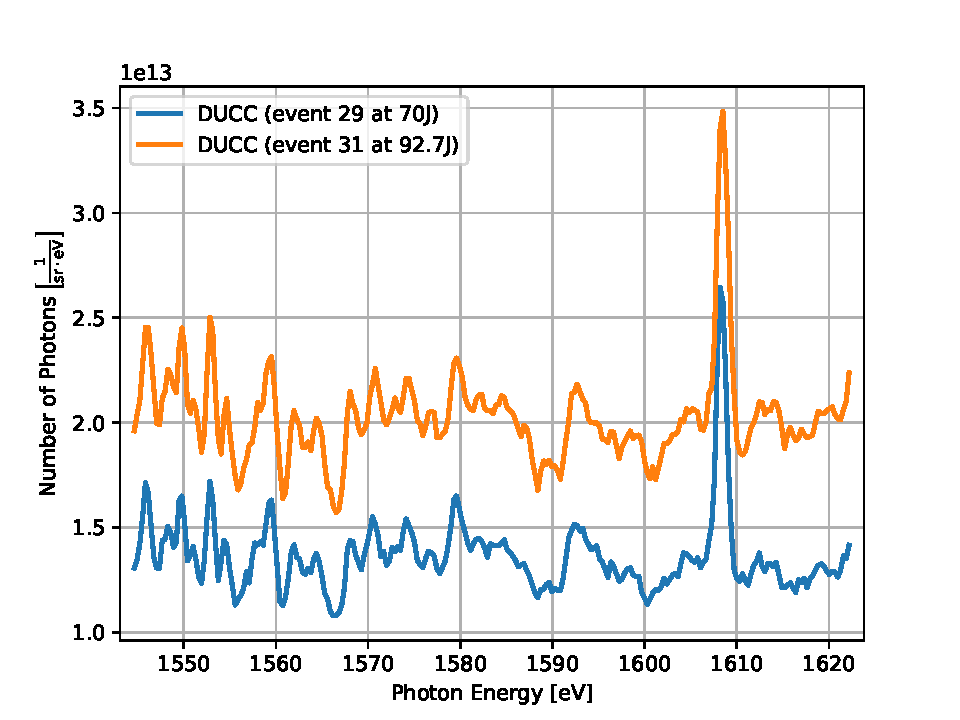
\includegraphics[width=\textwidth]{Data_Analysis/basic_spectra/spectra_of_Sm_events_29_31.pdf}
		\caption{Source spectra of samarium detected with the DUCC.}
		\label{}
	\end{subfigure}%
	\hfill
	\begin{subfigure}[t]{0.49\textwidth}
		\centering
		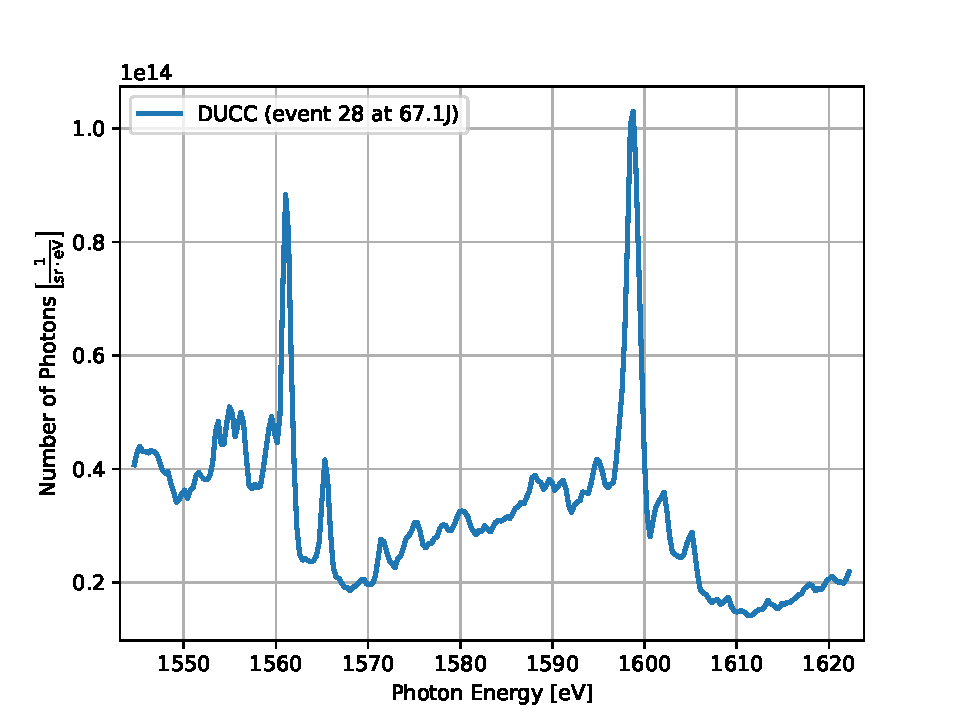
\includegraphics[width=\textwidth]{Data_Analysis/basic_spectra/basic_spectrum_of_Tb_event_28_on_DUCC.pdf}
		\caption{Source spectrum of terbium detected with the DUCC.}
		\label{}
	\end{subfigure}
	\begin{subfigure}[t]{0.49\textwidth}
		\centering
		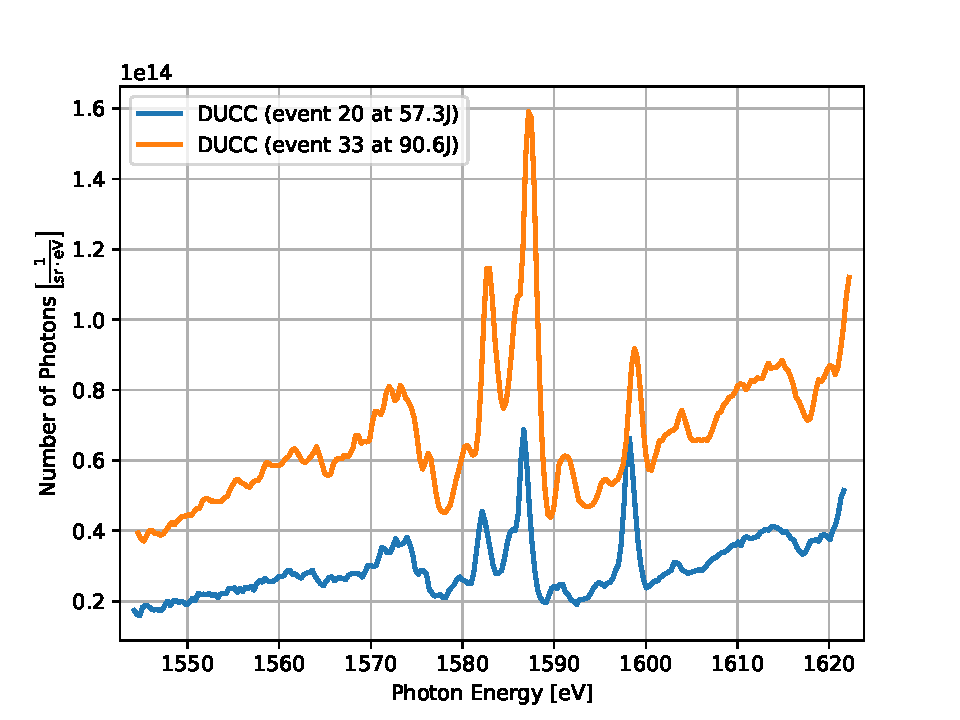
\includegraphics[width=\textwidth]{Data_Analysis/basic_spectra/spectra_of_Dy_events_20_33.pdf}
		\caption{Source spectra of dysprosium detected with the DUCC.}
		\label{}
	\end{subfigure}%
	\hfill
	\begin{subfigure}[t]{0.49\textwidth}
		\centering
		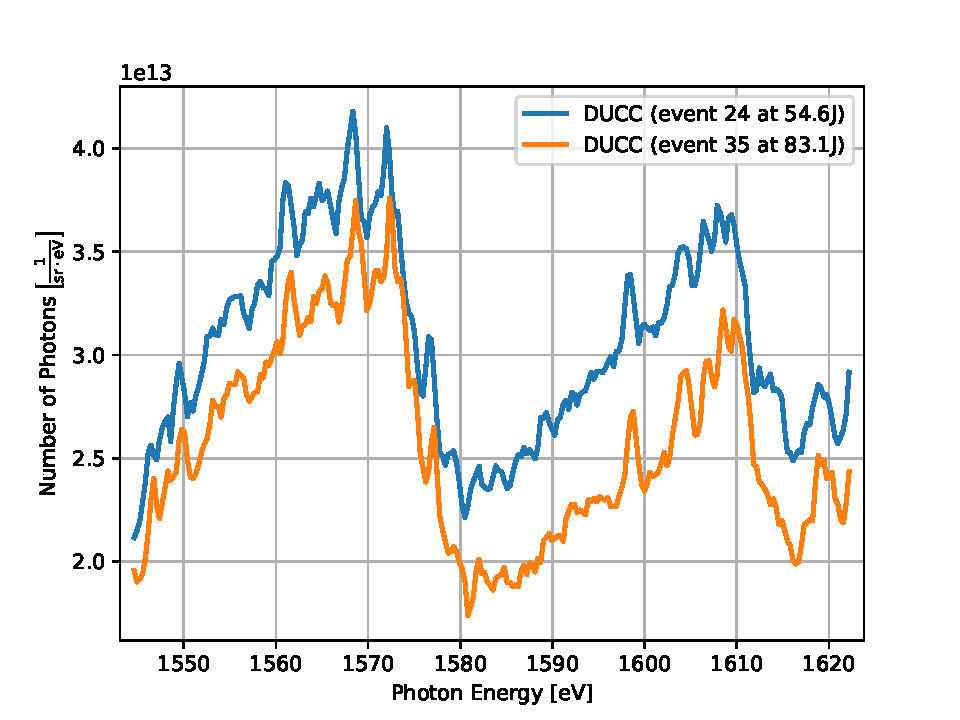
\includegraphics[width=\textwidth]{Data_Analysis/basic_spectra/spectra_of_Gd_events_24_35.pdf}
		\caption{Source spectra of gadolinium detected with the DUCC.}
		\label{}
	\end{subfigure}
	\begin{subfigure}[t]{0.49\textwidth}
		\centering
		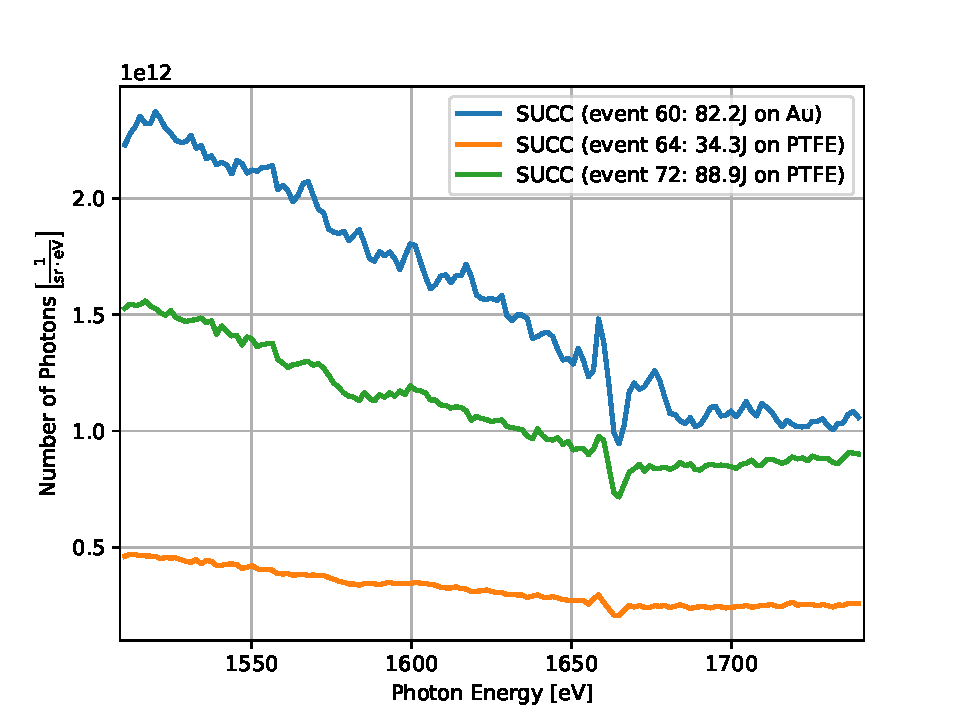
\includegraphics[width=\textwidth]{Data_Analysis/basic_spectra/spectra_of_PTFE_events_60_64_72.pdf}
		\caption{Source spectra of Teflon (PTFE) and gold detected with the SUCC.}
		\label{subfigure: PTFE basic spectra}
	\end{subfigure}%
	\hfill
	\begin{subfigure}[t]{0.49\textwidth}
		\centering
		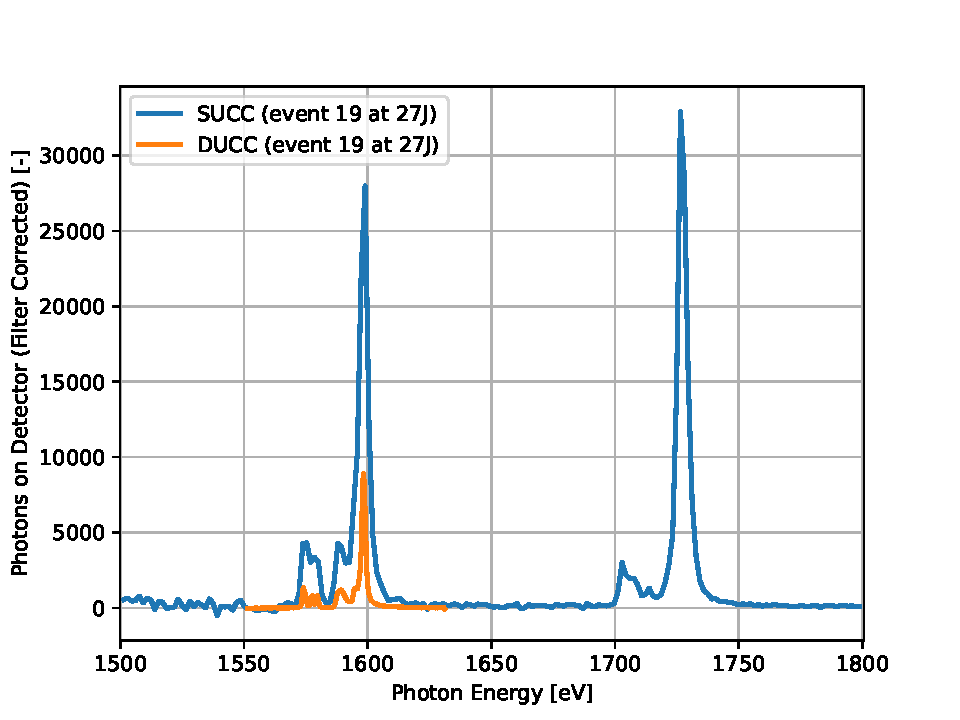
\includegraphics[width=\textwidth]{Data_Analysis/basic_spectra/spectra_of_Al_events_19_19.pdf}
		\caption{Source spectrum of aluminum detected with the DUCC and SUCC respectively.}
		\label{fig: Al DUCC series}
	\end{subfigure}
	\caption{Source spectra of laser-driven plasma from various backlighter materials. Shots of different laser energies are shown when available. Notably, the Teflon spectra are from the SUCC because the signal-to-noise ratio for the DUCC is in this case poor, as the intensity of the emission is at least an order of magnitude lower than for other backlighters.}
	\label{figure: basic spectra}
\end{figure}

In general, the spectrometers successfully produce results qualitatively in agreement with the expected source spectra. Each rare earth spectrum is dominated by high density line emission, recognizable in the peak-heavy structures, whereas the Teflon and gold spectra exhibit a quasi-continuous spectrum whose intensity falls with increasing photon energy, as is consistent with recombination or bremsstrahlung emission. Additionally, for backlighter materials with shots of various laser energies (see fig. \ref{figure: basic spectra}) the emission is stronger for greater laser energy, with the exception of gadolinium, where the \SI{54.6}{\joule} shot displays lower photon numbers than the \SI{83.1}{\joule} shot. The difference can be explained by the use of a phase plate in front of the PHELIX laser for the latter shot, which reduces the overall laser intensity. Overall, the consistency of the source spectra with expectations serves as a first validation of the spectrum processing procedure and the efficacy of the spectrometers.

\begin{figure} [H]
	\centering
	\begin{subfigure}[t]{0.7\textwidth}
		\centering
		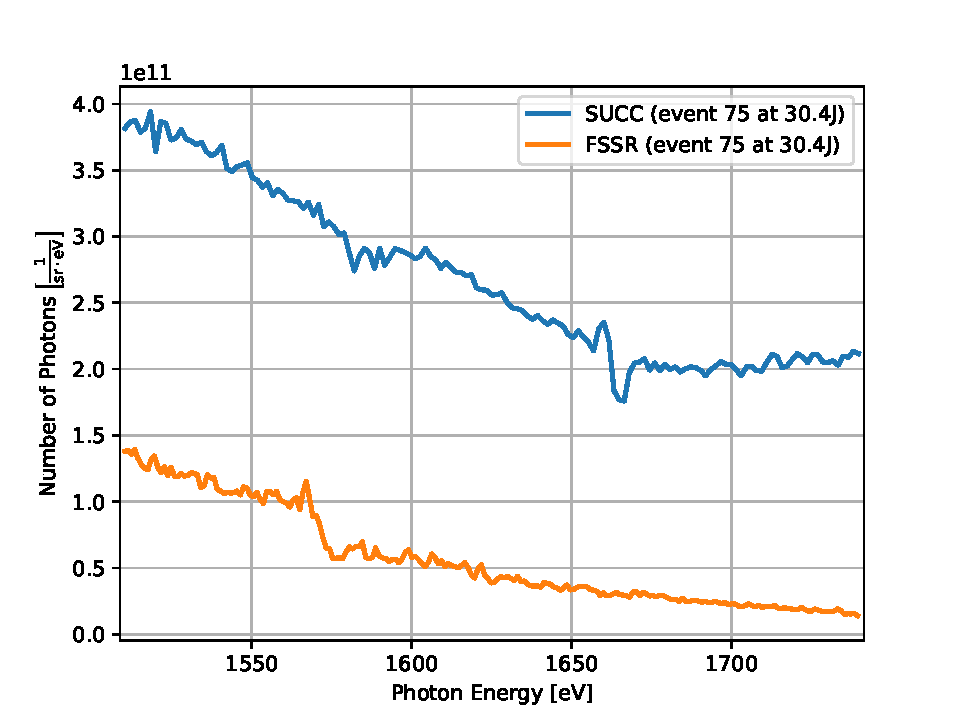
\includegraphics[width=\textwidth]{Data_Analysis/basic_spectra/spectra_of_PTFE_events_75_75.pdf}
		\caption{Source spectrum of Teflon detected with the FSSR and SUCC respectively.}
		\label{fig: FSSR basic spectrum}
	\end{subfigure}
	\hfill
	\begin{subfigure}[t]{\textwidth}
		\centering
		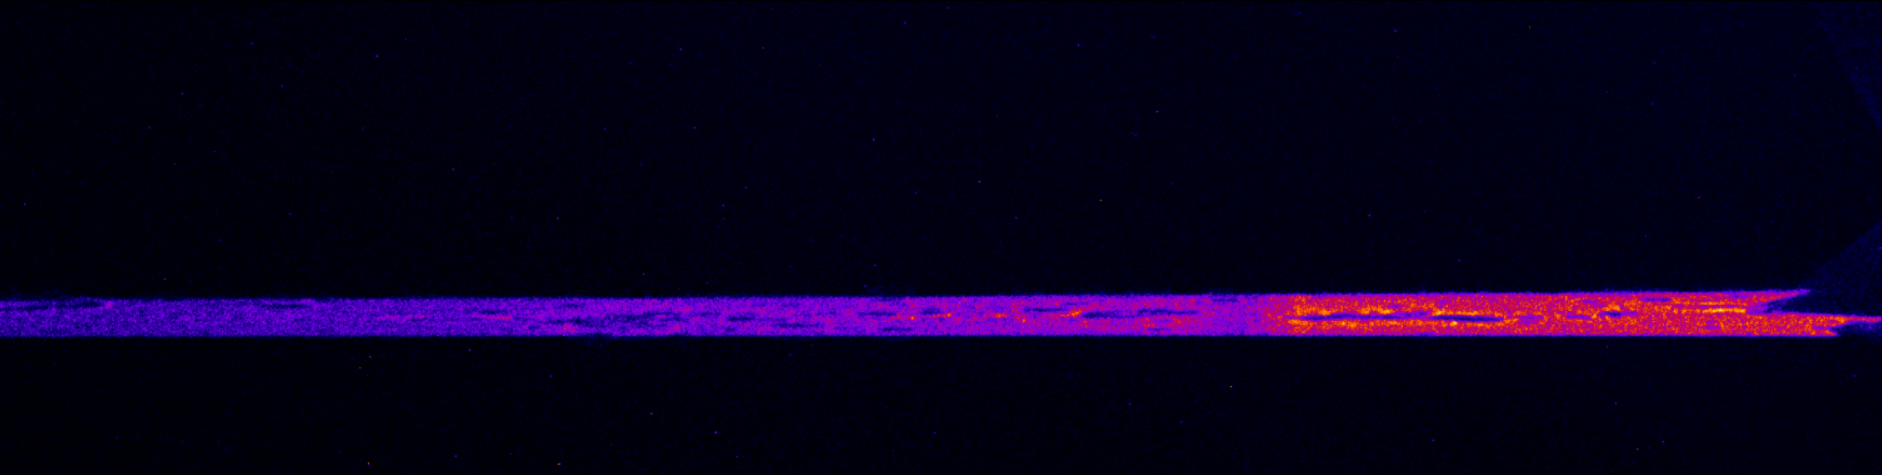
\includegraphics[width=\textwidth]{Data_Analysis/basic_spectra/FSSR_75.png}
		\caption{Raw TIFF image from the FSSR (unfocused) for a shot on Teflon at \SI{30.4}{\joule} (event 75).}
		\label{fig: FSSR TIFF}
	\end{subfigure}
	\caption{(a) shows the difference in spectra from a single shot on Teflon for different spectrometers. From this one can identify spectral features that most likely are linked to crystal defects and properties. Notable is the dip at $\approx$\SI{1570}{\electronvolt} in the spectrum from the FSSR, an artefact of the Al K-edge originating from the presence of aluminum in the mica crystal makeup. (b) is a TIFF image for the FSSR with a defocusing of \SI{5}{\milli\meter}, showing the numerous holes and deformations in the raw image of the FSSR, which are due to crystal defects and damage.}
	\label{}
\end{figure}

It is important to note that not all structures of the spectra are from the spectral properties of the emission. A significant source of spectral artefacts are the crystals, e.g. from defects in the lattice structure or outside influences, like dirt or imperfect adherence to the substrate. One example of such a spectral feature can be found in fig. \ref{subfigure: PTFE basic spectra}, where at approximately \SI{1660}{\electronvolt} there are a sudden rise and dip in all the spectra independent of the backlighter material. Such spectral features are also present and especially prevalent for the FSSR. As is apparent from fig. \ref{fig: FSSR basic spectrum}, the FSSR spectra are laden with features that are most likely caused by defects and properties of the spherically bent mica crystal, impacting the source spectrum. For example, a dip occurs for the FSSR at $\approx$\SI{1570}{\electronvolt}, preceded by a small peak at $\approx$\SI{1565}{\electronvolt}. These artefacts are likely caused by a K-edge from the aluminum component in the mica and by holes and features in the raw image (see fig. \ref{fig: FSSR TIFF}) that can be traced back to defects in the crystal. To note is that for a standard FSSR-1D setup, the signal would appear as a single horizontal line. In this case, the image was unfocused by extending the crystal-detector distance $b_0$ by \SI{5}{\milli\meter}, shifting the detector away from the Rowland circle.  Besides the difficulties of the crystal quality, the FSSR performed qualitatively as designed in that the predicted focusing properties were successfully reproduced and that spectra with the expected dispersion were extracted.

\subsection{X-ray Absorption Spectra}
\label{subsection: ab spectra}

The processing of the x-ray absorption spectra begins with the extraction of the spectra for a given absorption shot analogously to the previous section, yielding a source and transmitted spectrum from the same x-ray source. The two spectra are then aligned with an algorithm that shifts the source spectrum until the best possible alignment is found in a given energy range; a step made necessary by small shot-to-shot deviations of the x-ray source position. Once aligned, the photon energy dependent transmission $T(E)$ is calculated by the ratio of the transmitted intensity $I_{trans}$ to the source spectrum intensity $I_{source}$. The absorption coefficient $\mu$ can then be determined with the equation 
\begin{equation}
	\mu = \frac{-\ln(T)}{d_{Al,eff}},
\end{equation}
where the effective aluminum thickness $d_{Al,eff}$ takes into account the angle of the x-rays to the sample surface. The sample material was provided with an error of 10\% for $d_{Al}$, which gets passed onto the absorption coefficient using Gaussian error propagation.

While this procedure is effective for crystals of excellent quality, the processing can be improved by including a crystal calibration step. This step consists of using a calibration shot, in which spectra without a sample are taken with ideally the same setup and laser parameters as the absorption shot, in order to account for spectral features from crystal defects. In this case, the transmission is calculated by
\begin{equation}
	T = \frac{(I_{trans}/I_{source})}{(I_{cal,trans}/I_{cal,source})},
\end{equation}
where $I_{cal,trans}$ and $I_{cal,source}$ are the calibration spectra corresponding to the spectrometers/spectrometer channels of the transmitted and source spectrum of the absorption shot. To note is that this calibration introduces further complexity to the processing and hinges on how accurately the shots are reproduced, i.e. with low fluctuation of the x-ray source position and same backlighter at similar laser energy. Accordingly, I chose to apply this crystal calibration to the OSUCC/SUCC absorption shot, since the spectrometers are not identical and the crystals were of differing quality. I did not apply this calibration to the shots with the DUCC as no suitable calibration shots exist and the ADP crystals were of relatively good quality, in that they display few noticeable spectral features.

For all the results presented, the Al sample was placed directly on the spectrometer channel entrance to ensure that the Al foil remained at ambient temperature, i.e. so that no preheating due to proximity to the backlighter occurs. The experimental results are validated by an Al absorption spectrum published by \textit{Levy et al.} \citep{levy2010double}, whose experimental setup is similar to our own with the DUCC, with the key differences that they used erbium as backlighter and conically-bent crystals for their spectrometer



\begin{figure} [!htbp]
	\centering
	\begin{subfigure}[t]{0.88\textwidth}
		\centering
		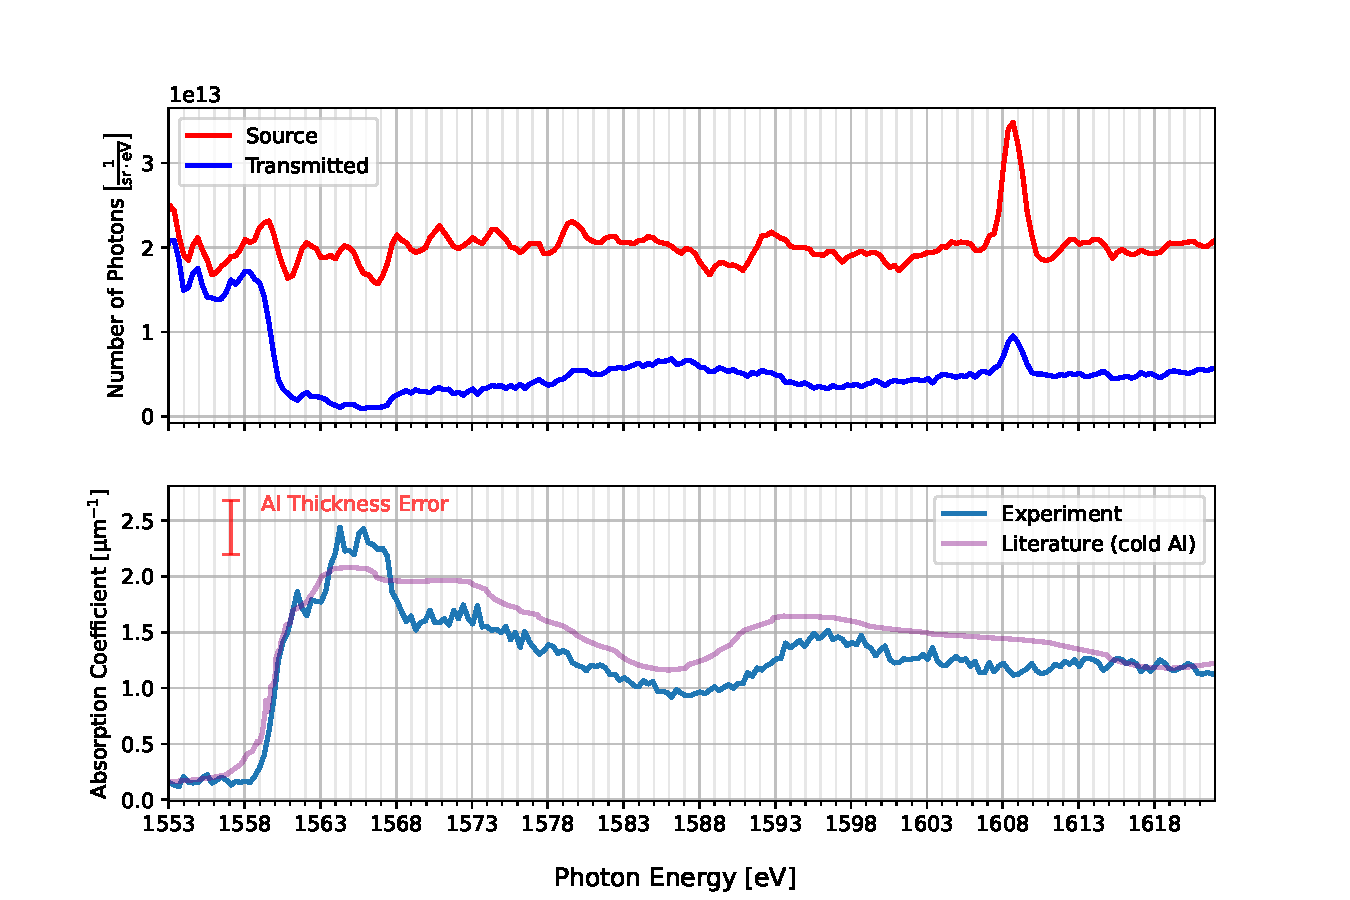
\includegraphics[width=\textwidth]{Data_Analysis/absorption_wo_calibration/absorption_spectrum_of_Sm_event_31_on_DUCC.pdf}
		\caption{X-ray absorption spectrum through a \SI{1.18\pm0.12}{\micro\meter} thick aluminum foil for a \SI{97.4}{\joule} shot on samarium.}
		\label{fig: DUCC absorption Sm}
	\end{subfigure}%
	\hfill
	\begin{subfigure}[t]{0.88\textwidth}
		\centering
		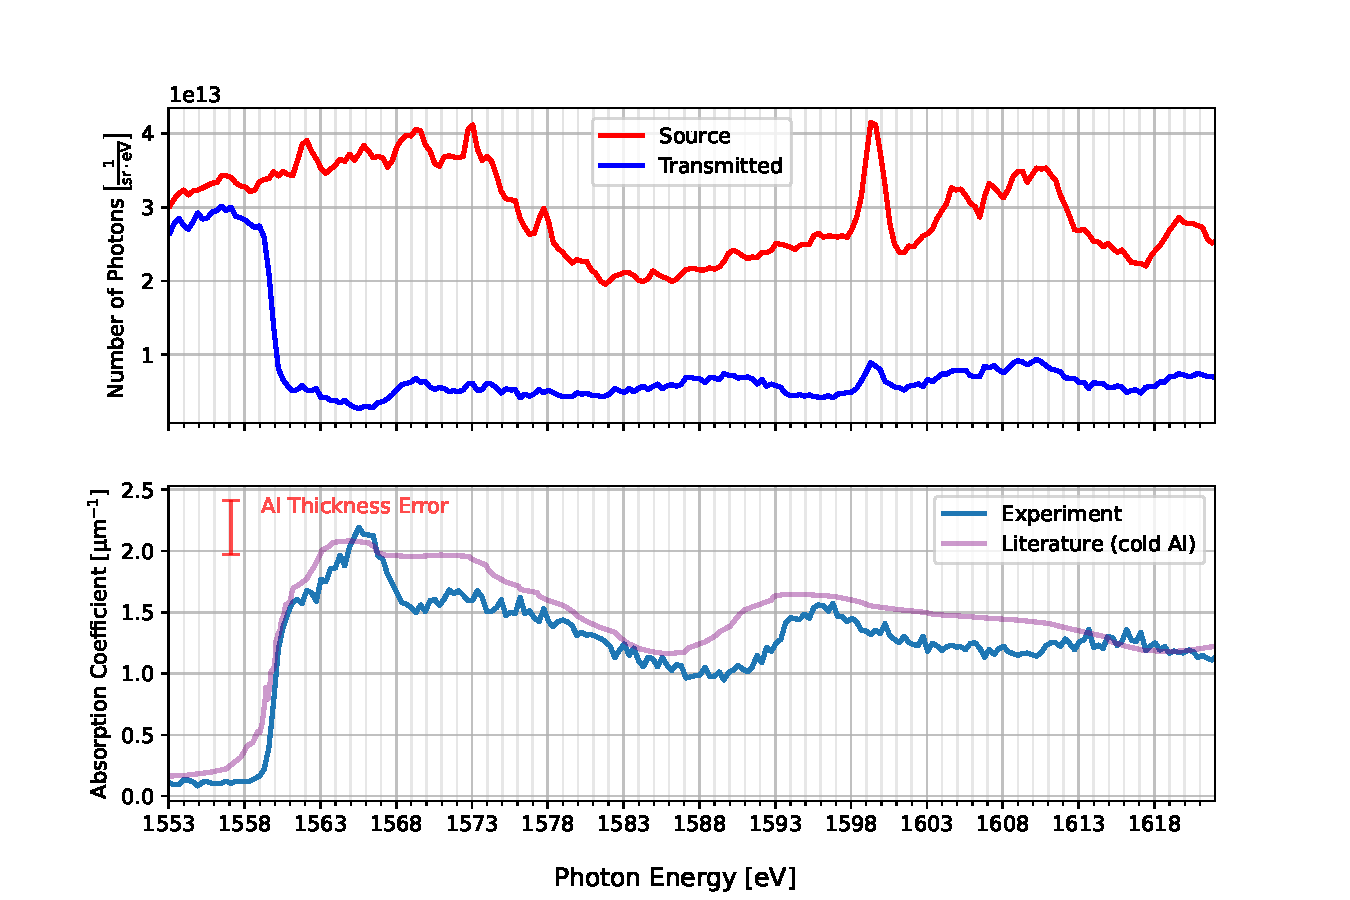
\includegraphics[width=\textwidth]{Data_Analysis/absorption_wo_calibration/absorption_spectrum_of_Gd_event_32_on_DUCC.pdf}
		\caption{X-ray absorption spectrum through a \SI{1.18\pm0.12}{\micro\meter} thick aluminum foil for a \SI{87.4}{\joule} shot on gadolinium.}
		\label{fig: DUCC absorption Gd}
	\end{subfigure}
	\caption{X-ray absorption spectra detected with the DUCC. In (a) and (b); \textbf{Top:} fully processed spectrum pair whose ratio yields the x-ray transmission through the sample. \textbf{Bottom:} absorption spectrum with comparison to a result from \textit{Levy et al.} \citep{levy2010double} and the systematic uncertainty due to the sample thickness, depicted as an error bar that aligns with the maximum value of $\mu$.}
	\label{fig: DUCC absorption}
\end{figure}

The absorption spectra of fig. \ref{fig: DUCC absorption} and \ref{fig: SUCC absorption} both exhibit reasonable agreement with the literature, with the absorption curves of the SUCC/OSUCC setup, where the first spectrometer detects the source spectrum and the second the transmitted, showing closer agreement then the spectra from the DUCC. As such, the absorption curves were successfully extracted, albeit with varying quality dependent on the spectrometer combination.

In the case of the absorption shots with the DUCC (see fig. \ref{fig: DUCC absorption}), for which the dual channels are employed to record the spectra, a reasonably good agreement with the literature curve is achieved, considering that no crystal calibration is carried out and that the transmitted and source spectra are structure-heavy. In fact, much of the structure in the absorption spectra can attributed to features of the x-ray source emission. In general, a peak in the source spectrum will yield a dip in the absorption, and vice-versa. For example, many structures occur in the range of 1561-\SI{1568}{\electronvolt} that are clearly artefacts from the source spectrum, a observation supported by the difference of the absorption curves in that range between fig. \ref{fig: DUCC absorption Sm} and fig. \ref{fig: DUCC absorption Gd}. This implies that the processing procedure for the absorption spectrum does not fully eliminate the spectral structures of the backlighter, which could be remedied by further refinement of the transmission calculation or by carrying out a crystal calibration, since the reflectivity of the two ADP crystals are likely to vary slightly depending on photon energy. Despite these deviations, the similarity of the overall behavior of the experimental absorption spectra from the DUCC, especially in the oscillation after \SI{1570}{\electronvolt}, implies qualitative consistency between shots, lending validity to the experimental setup and dual channel spectrometer design.


The two shots in fig. \ref{fig: DUCC absorption} also differ from the literature example in the magnitude of the absorption coefficient, with the experimental curve being on average lower, as well as in the dip at \SI{1568}{\electronvolt} and the location of the second peak of the oscillation at \SI{1593}{\electronvolt}. The error due to the Al sample thickness could explain the former difference. For the latter, the extra dip at \SI{1568}{\electronvolt} in the experimental absorption curve is likely due to the influence of sample thickness on XANES structures, which is illustrated in fig. 6 of the paper from \textit{Levy et al.} \citep{levy2010double}. This idea is further supported by the closer agreement of the absorption spectrum detected with the SUCC/OSUCC (see fig. \ref{fig: SUCC absorption}), where the geometry leads to a smaller effective sample thickness of \SI{0.84\pm0.08}{\micro\meter}. On the other hand, the different location of the second oscillation peak at \SI{1593}{\electronvolt} could be explained by differences in experimental setup, e.g. in the x-ray source or sample, as the deviation between the literature and experimental curve appears in all shots. The cause of both the differences should be investigated by further literature research and comparison to Al absorption curves of other experiments.

\begin{figure}[!htbp]
	\centering
	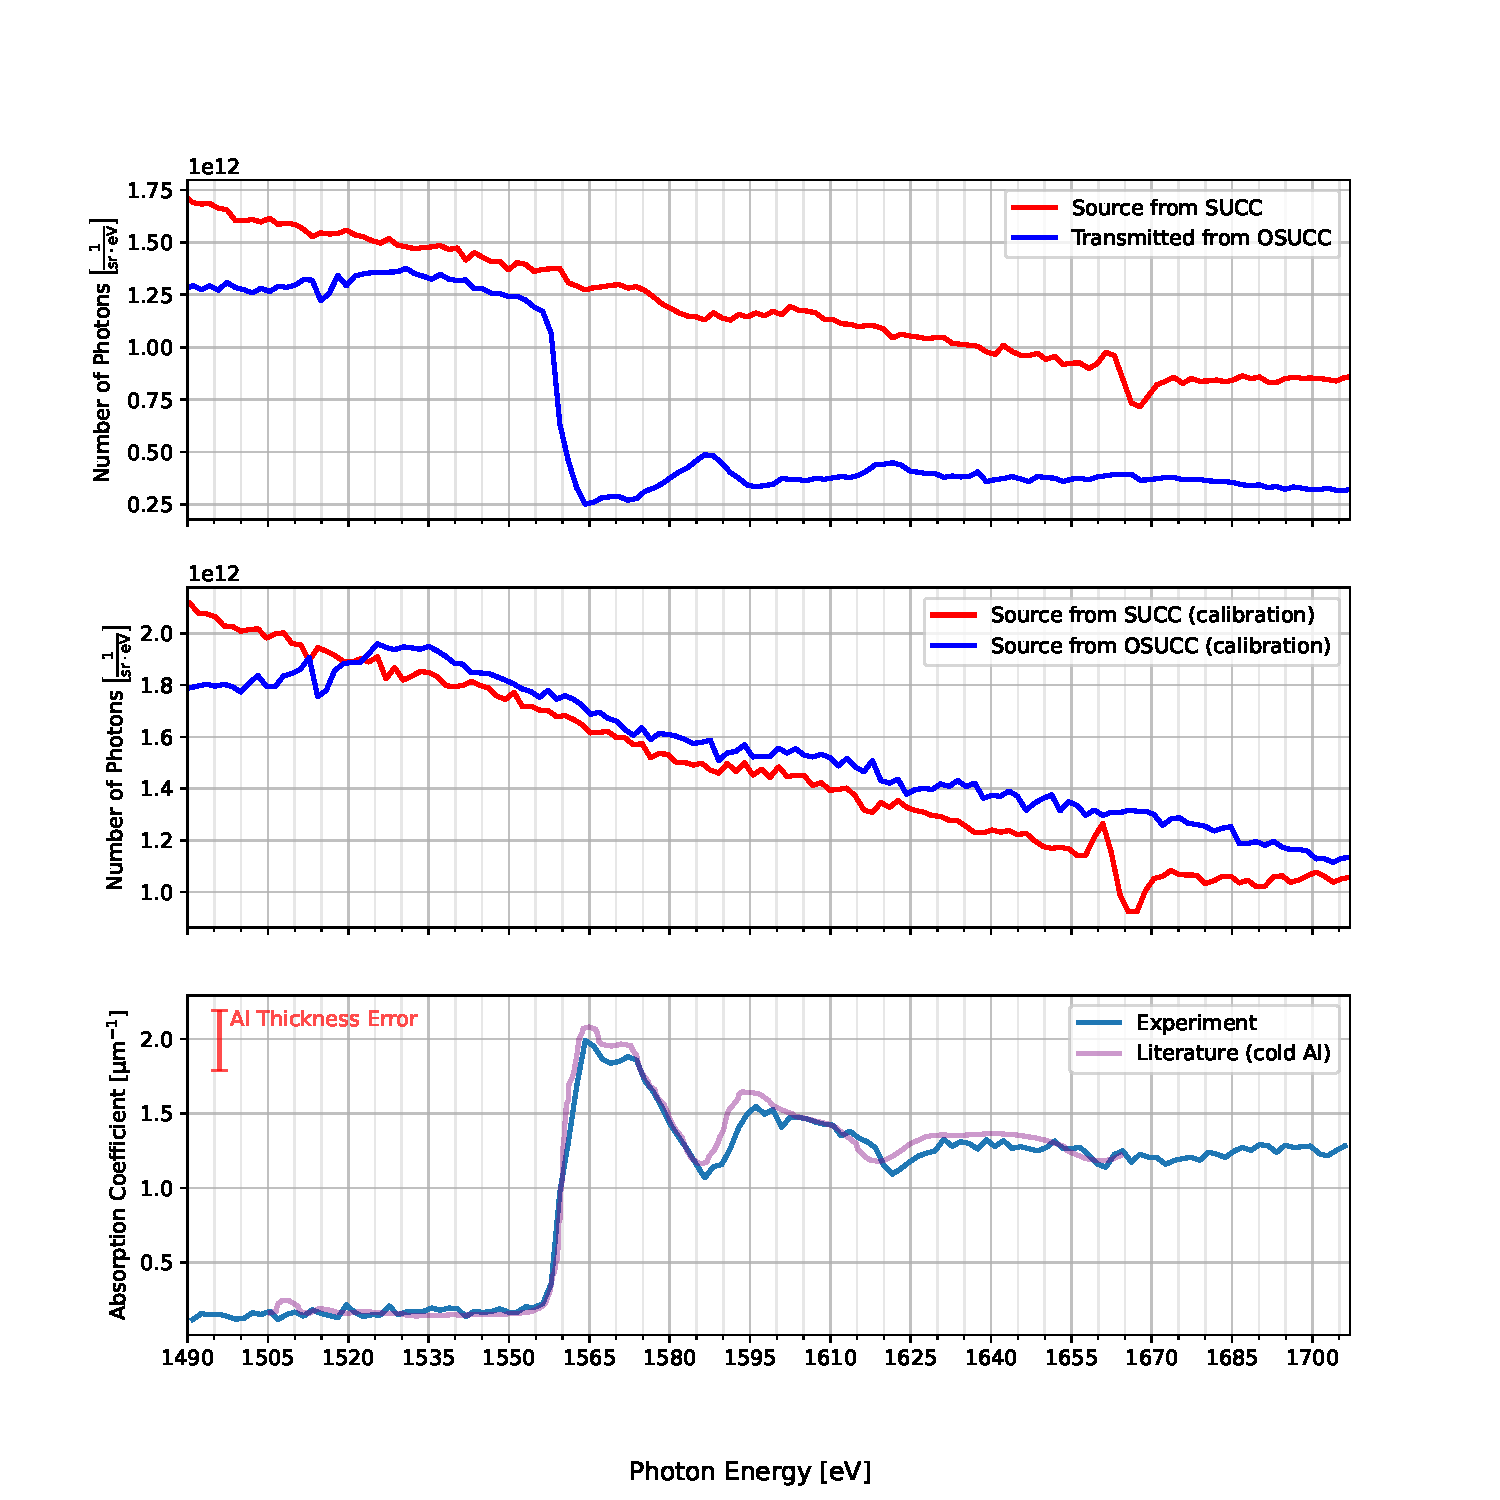
\includegraphics[width=\textwidth]{Data_Analysis/absorption/absorption_spectrum_of_PTFE_event_72_on_OSUCC.pdf}
	\caption{X-ray absorption spectrum detected with the SUCC for the source and the OSUCC for the transmitted spectrum. The crystal spectral features are corrected out using a calibration shot without a sample. \textbf{Top:} fully processed spectrum pair from a \SI{88.9}{\joule} shot on Teflon. The ratio of transmitted to source spectrum along with the crystal calibration yields the x-ray transmission through a \SI{0.84\pm0.08}{\micro\meter} thick aluminum foil sample. \textbf{Middle:} fully processed calibration spectrum pair from a \SI{110.3}{\joule} shot on Teflon. \textbf{Bottom:} absorption spectrum with comparison to a result from \textit{Levy et al.} \citep{levy2010double} and the systematic uncertainty due to the sample thickness, depicted as an error bar that aligns with the maximum value of $\mu$.}
	\label{fig: SUCC absorption}
\end{figure}

In contrast to the DUCC, the absorption spectrum pictured in fig. \ref{fig: SUCC absorption} is extracted using two separate single channel spectrometers, namely the SUCC and OSUCC, and a Teflon backlighter, which displays an exceptionally smooth x-ray source spectrum. Interestingly, the resulting absorption curve shows overall excellent agreement with the literature except for slight deviations of a few eV for the oscillation's peaks and valleys after \SI{1580}{\electronvolt}, which could be explained by experimental setup differences analogously to the discussion of the DUCC's second peak. The agreement occurs despite the fact that the KAP crystal of the OSUCC was of visibly low quality, especially apparent in the calibration spectra below \SI{1530}{\electronvolt}, and that the spectral resolutions are by nature of the spectrometer geometries different. I attribute the effectiveness of the setup to three considerations. First, the crystal features in the recorded spectra are for the most part corrected out by the crystal calibration, as apparent in the disappearance of the peak and valley around \SI{1665}{\electronvolt} inherent in both the calibration and source spectrum of the SUCC. Second, the smoothness of the Teflon spectra suppresses the difference of spectral resolutions, while reducing overall foreign structure in the absorption curve. Third, the OSUCC crystal's strongest spectral features, visible in the calibration spectrum of the OSUCC, occur below the K-edge, such that they have no influence on the fine-structures on the absorption curve. Therefore, the resulting quality of the experimental absorption spectrum demonstrates the power of a smooth backlighter spectrum as well as the crystal calibration method.

The spectrometer combination employing the SUCC/FSSR was unsuccessful, where an example with a teflon backlighter is shown in fig. \ref{fig: FSSR absorption}. Despite many attempts at tuning the alignment algorithm and selecting a suitable combination of absorption and calibration shots, the absorption spectra derived from the SUCC/FSSR setup yielded no curves that clearly aligned with that of aluminum. The main reasons are twofold. On one hand, the poor quality of the mica crystal and presence of Al in the chemical makeup lead to significant spectral structure around the K-edge energy, heavily distorting the absorption curve, especially at the edge. On the other, the vastly different geometries and function of the FSSR and SUCC hindered the aligning of the component spectra and prevented the removal of spectral structures in the absorption curve, which is most noticeable at large peaks in the backlighter emission, excluding the use of rare-earth backlighters. The difference in spectral resolution has the largest impact in this regard. Even for Teflon backlighters, the absorption spectra were not successfully extracted with the SUCC/FSSR combination (see fig. \ref{fig: FSSR absorption}). This result reflects the importance of good crystal quality, even with a meaningful tool like the crystal calibration, and similarity of the spectrometer geometries.

In summary, high quality absorption spectra are successfully extracted by the DUCC with rare-earth backlighters and the SUCC/OSUCC with Teflon, where the latter combination is closer to the literature. The SUCC/FSSR spectrometer combination does not yield viable absorption curves, even with Teflon backlighters. Accordingly, using the same spectrometers for both the source and transmitted spectra is desirable, meaning that the DUCC geometry represents the most promising setup. Additionally, the flat crystals are capable of producing low-noise, well resolved absorption spectra, as demonstrated by both the ADP crystals of the DUCC and the KAP of the SUCC/OSUCC. A smooth backlighter spectrum is also important for the quality of the absorption curves, since it simplifies processing and smooths the final absorption spectra, though the chosen x-ray source must suit the crystal, as shown by the incompatibility of Teflon backlighters with ADP. As such, combining the DUCC geometry with KAP crystals presents a promising solution, enabling the use of Teflon backlighters as well as identical geometries for the source and transmitted spectra.


\begin{figure}[H]
	\centering
	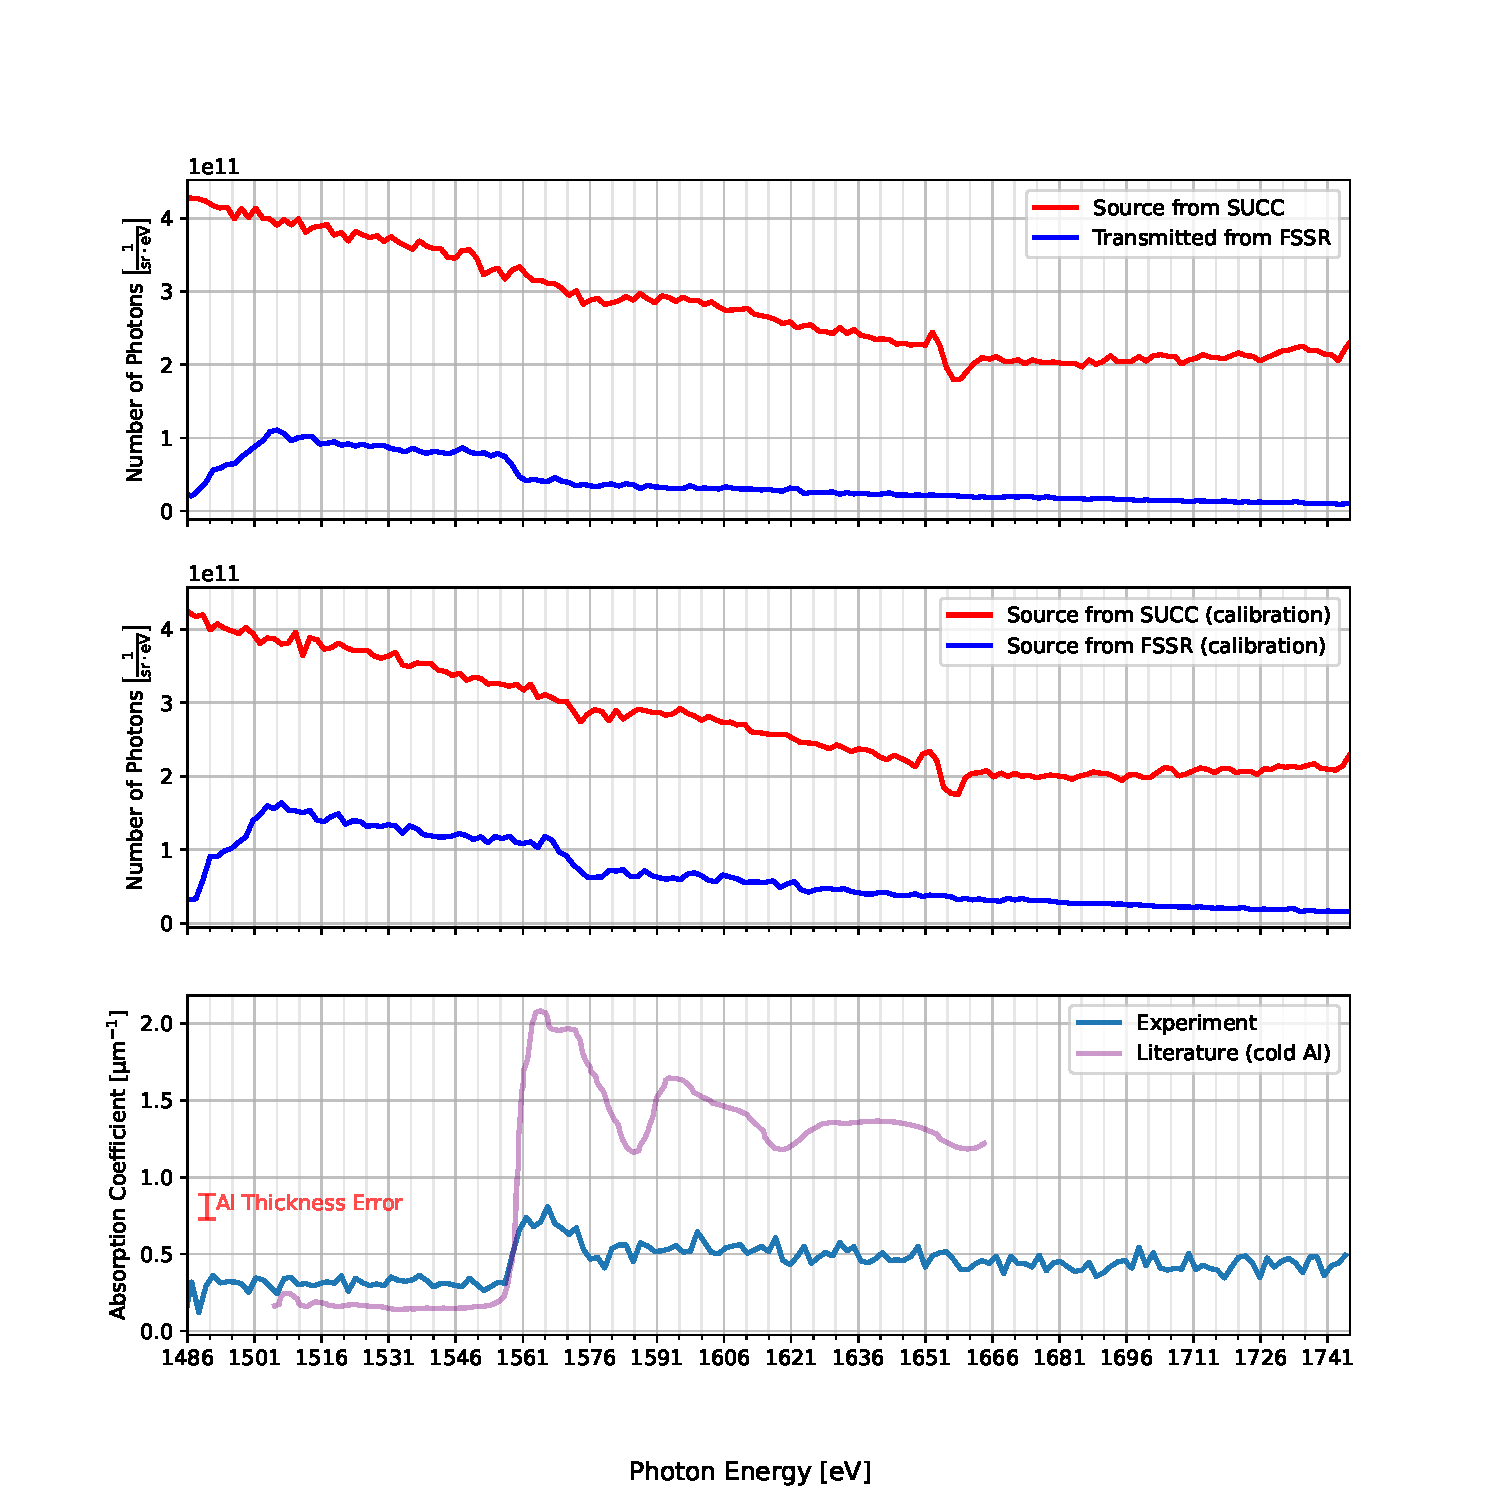
\includegraphics[width=\textwidth]{Data_Analysis/absorption/absorption_spectrum_of_PTFE_event_74_on_FSSR.pdf}
	\caption{X-ray absorption spectrum detected with the SUCC for the source and the FSSR for the transmitted spectrum. The crystal spectral features are corrected out using a calibration shot without a sample. \textbf{Top:} fully processed spectrum pair from a \SI{30.8}{\joule} shot on Teflon. The ratio of transmitted to source spectrum along with the crystal calibration yields the x-ray transmission through a \SI{1.0\pm0.1}{\micro\meter} thick aluminum foil sample. \textbf{Middle:} fully processed calibration spectrum pair from a \SI{30.4}{\joule} shot on Teflon. \textbf{Bottom:} absorption spectrum with comparison to a result from \textit{Levy et al.} \citep{levy2010double} and the systematic uncertainty due to the sample thickness, depicted as an error bar that aligns with the maximum value of $\mu$.}
	\label{fig: FSSR absorption}
\end{figure}


\section{Spectrometer Characterization}
\label{section: spectrometer characterization}

To perform a quantitative analysis of the spectrometer performance, properties of three spectrometers, namely the DUCC, FSSR, and SUCC, will be investigated, giving insight into the extent to which the designs were successfully implemented. First, I will calculate the ratio of the integrated reflectivities of the crystals for each spectrometer pairing, as well as infer the $R_{int}$ value of the mica crystal in the FSSR with the help of a simulation carried out by Artem Martynenko, allowing further characterization of the crystals and assessment of their impact on the spectrometers' performance. Second, the spectral resolution and its contributions will be determined for all the spectrometers using the He-$\upalpha$ line emission of aluminum, along with the steepness of the K-edge in transmission spectra of Al recorded with the DUCC. From these results, I will assess the efficacy of the \textit{mmpxrt} simulations and the viability of each spectrometer for its intended variant of XAFS.

In this section the crystal properties play a crucial role and therefore will be further elaborated on. As discussed in section \ref{section: resolution theory}, the relevant parameters are the integrated reflectivity $R_{int}$ and the rocking curve width $\Delta \theta$, which both are determined from a reflection curve at a given photon energy. $R_{int}$ parameterizes the reflectivity of the crystal, i.e. how many of the monochromatic photons are reflected, so that a larger $R_{int}$ implies a higher luminosity of the spectrometer, while $\Delta \theta$ gives the width of the reflection curve and impacts the spectral resolution of the spectrometer \citep{holzer1998flat}. In general, the more defects in a crystal the higher the integrated reflectivity and $\Delta \theta$. An important property of the integrated reflectivity is its independence from the x-ray source properties, like beam size, and shape of the reflection curve \citep{loisel2016measurement}. Because of this and the indirect relation of the two crystal properties, I will study $R_{int}$ and the spectral resolution separately.

Generally speaking, it is difficult to estimate $R_{int}$ and $\Delta \theta$ for a given crystal without directly measuring, since the quantities are highly sensitive to crystal quality, i.e. the density of crystal defects, and depend on the refraction order and photon energy \citep{ferrari2019characterization}, leading to significant variance among the literature. A good example of this is for ADP crystals, where integrated reflectivities can vary by an order of magnitude, as with the values \SI{2.32}{\micro\radian} \citep{ferrari2019characterization} and \SI{40}{\micro\radian} \citep{gilfrich1975integral}. Consequently, in section \ref{section: int refl ratio} the assumed values of the crystal properties will be adjusted according to new information gathered from Artem's simulation as well as experimental results, with which additional \textit{mmpxrt} simulations will be conducted and used to discuss the spectral resolutions of section \ref{subsection: spectral resolution}.

\subsection{Integrated Reflectivity Ratio}
\label{section: int refl ratio}

To build on the findings of the previous section, the ratio of $R_{int}$ between different crystals will now be determined, giving a deeper insight into the quality of the KAP, ADP, and mica crystals. I begin by extracting the source spectra of a shot on Al for two spectrometers, following the same process as described in chapter \ref{chapter: data analysis} but leaving out the binning and multiplying equation \ref{conversion to emitted photons} with $R_{int}$, $\Delta E$ and 4$\pi$. The quantity of interest becomes the integral over the $N_{\text{total}}\cdot R_{int}$ values for a given energy range, which I chose to cover the two emission lines at \SI{1588.3}{\electronvolt} and \SI{1598.4}{\electronvolt}, corresponding to the $n=2\rightarrow n=1$ transitions of heliumlike ions of aluminum \citep{thompson2001x}. An example of an integration area is given in fig. \ref{fig: R_int DUCC_t}, with the other cases available in the appendix section \ref{appendix: supplementary results}.\ref{appendix: integrated reflectivity ratio}. These lines are selected because they are the strongest that fall within the shared energy range of every spectrometer. The integral is approximated by summing, yielding
\begin{equation}
	\sum_{i}N_{\text{total}}(E_i)\cdot R_{int} = \frac{\sum_{i}[4\pi\cdot N_{\text{det}}(E_i)\cdot D(E_i)]}{\Delta x_{\text{pix}}},
	\label{eq: ratio of R_int}
\end{equation}
where as in chapter \ref{chapter: data analysis} $\Delta x_{\text{pix}}$ becomes $w_{\text{crystal}}$ for the FSSR. Next, by simply taking the ratio of the integral for both spectrometers of a shot, I can determine the integrated reflectivity ratio of the crystals. As previously noted, $R_{int}$ cannot be directly measured by this setup due to the unknown total number of emitted photons from the source $N_{\text{total}}$.

\begin{figure}[H]
	\centering
	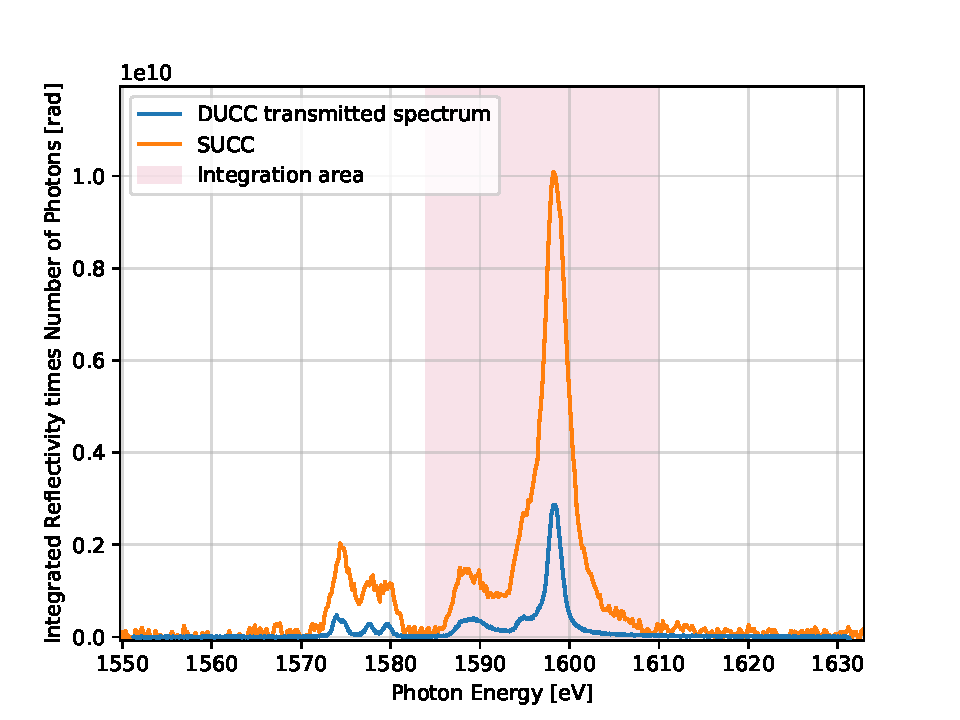
\includegraphics[width=0.8\textwidth]{Data_Analysis/R_int_ratio/spectra_of_Al_event_19_transmitted.pdf}
	\caption{$R_{int}\cdot N_\text{{total}}$ for a \SI{27}{\joule} shot on aluminum (event 19). The spectra from the transmission channel of the DUCC and the SUCC are presented, as well as the integration area used to calculate the integrated reflectivity ratio.}
	\label{fig: R_int DUCC_t}
\end{figure}

In addition to the method above, the $R_{int}$ for the mica crystal of the FSSR will be calculated directly by using the efficiency $\gamma$ of the FSSR spectrometer with mica crystal, derived in a simulation conducted by Artem Martynenko using the parameters of the FSSR geometry of this work and mica crystals typical of Sergey Pikuz' lab, where the crystal of this experiment originates. The efficiency is defined as the ratio the simulated photons reaching the detector $N_{\text{det,sim}}$ and the total number of emitted photons $N_{\text{total,sim}}$, i.e. $N_{\text{det,sim}}/N_{\text{total,sim}}$. I determine the integrated reflectivity of the FSSR by first linearly interpolating the efficiency data of fig. \ref{fig: efficiency graph} to get $\gamma(E)$. Then, equation \ref{eq: ratio of R_int} is applied to derive
\begin{equation}
	R_{int} = \frac{\sum_{i}[4\pi\cdot N_{\text{det}}(E_i)\cdot D(E_i)]/w_{\text{crystal}}}{\sum_{j}(N_{\text{det}}(E_j)/\gamma(E_j))},
\end{equation}
where the summations are over the same energy range described in the first method.



\begin{figure}[H]
	\centering
	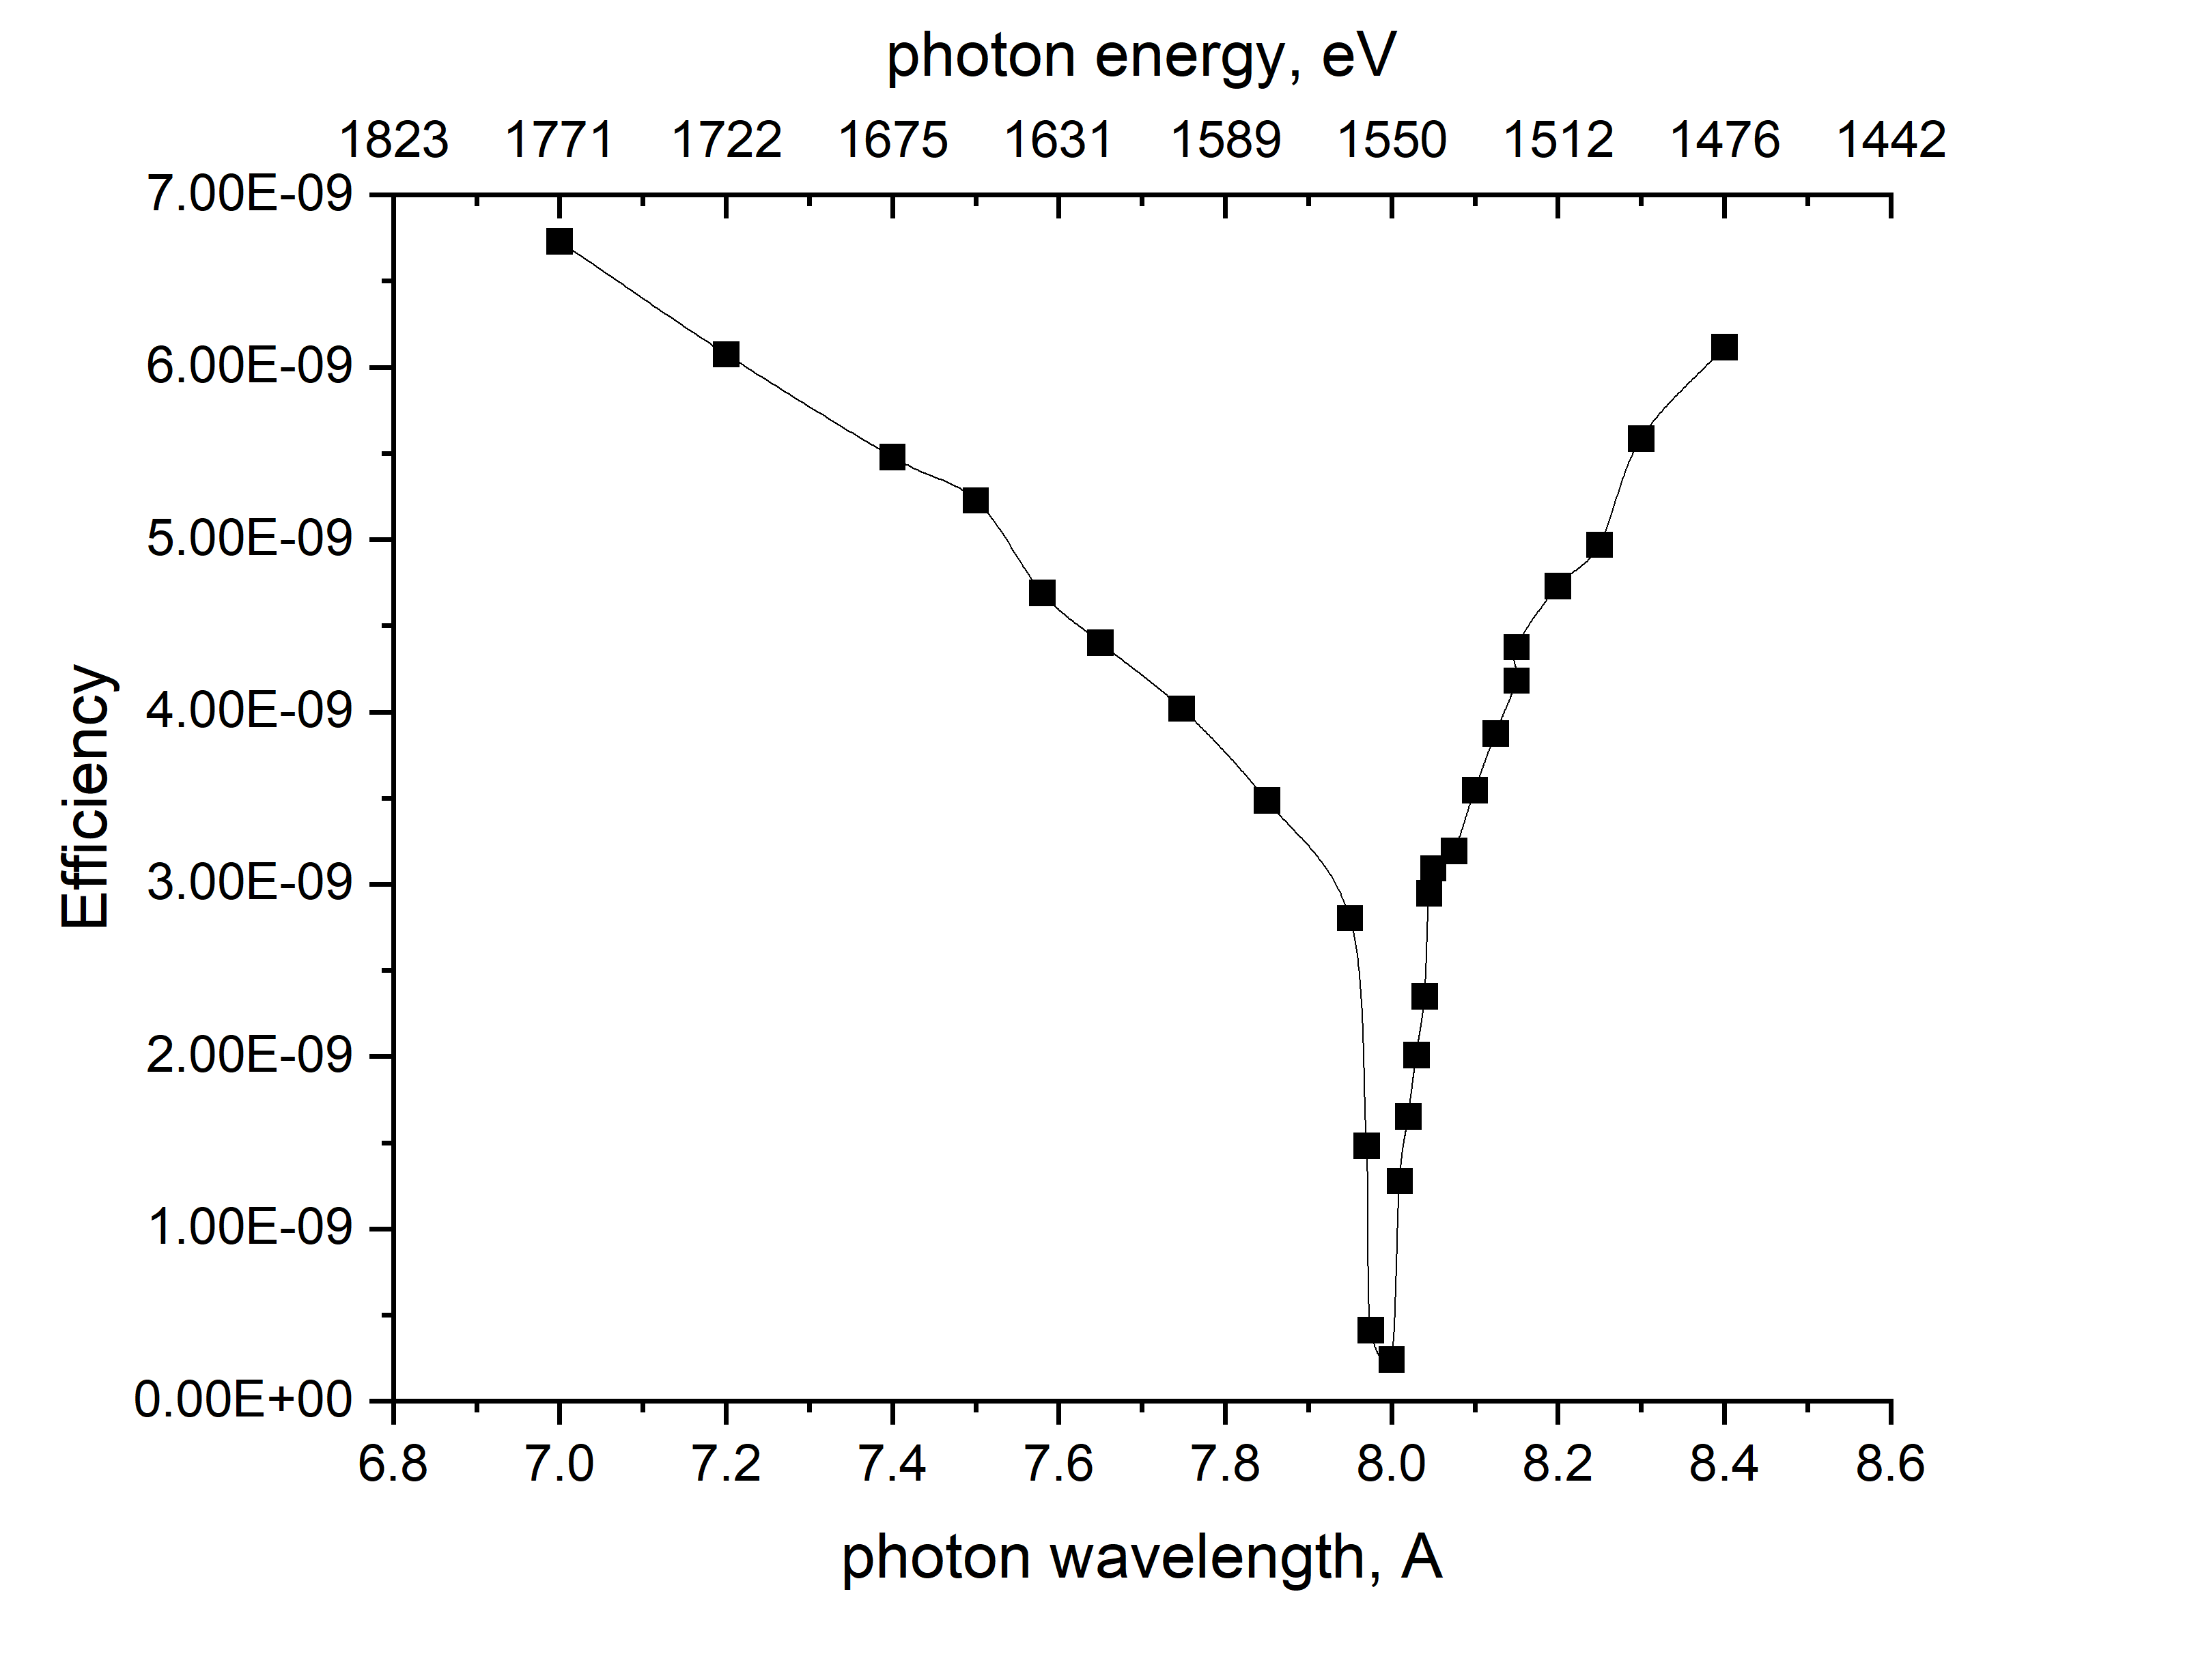
\includegraphics[width=0.8\textwidth]{Data_Analysis/efficiency_graph.png}
	\caption{Efficiency of the FSSR-1D with a mica crystal typical of Sergey Pikuz' lab, extracted by a ray tracing simulation carried out by Artem Martynenko. Immediately recognizable is a dip around 1540-\SI{1560}{\electronvolt}, which is related to the K-edge of the aluminum component of the mica crystal.}
	\label{fig: efficiency graph}
\end{figure}

The results will be compared to the estimated literature values for $R_{int}$ of \SI{40}{\micro\radian} for the ADP crystals of the DUCC \citep{gilfrich1975integral}, \SI{80}{\micro\radian} for the KAP crystal of the SUCC \citep{loisel2016measurement}, and \SI{53.6}{\micro\radian} for the mica crystal of the FSSR \citep{holzer1998flat}. In this case, \SI{40}{\micro\radian} is chosen over the value of \SI{2.32}{\micro\radian} used in the \textit{mmpxrt} simulations of section \ref{section: specs and comparison} because it lies closer to the experimental results in table \ref{Table: Rint Ratio}.

The results in table \ref{Table: Rint Ratio} for the experimentally determined ratios of the DUCC to the SUCC lie close to 1 and deviate from the expected values by less than a factor of 2, indicating that the ADP crystals have a $R_{int}$ larger than the literature value, the KAP crystals of the SUCC exhibit a lower integrated reflectivity, or some combination of the two. Interestingly, this also points to the ADP and KAP crystals having comparable integrated reflectivities, from which one would intuitively expect that the signal intensities on detector be similar, but the fact that the signal-to-noise ratio of the teflon backlighter/DUCC combination is too low to be feasible refutes this expectation. The difference between the photon intensity on the DUCC and SUCC can be explained by the difference in energy range, where the DUCC collects photons on more pixels for a given energy interval than the SUCC, reducing the overall photon count per pixel. Another interesting observation is that the DUCC/SUCC ratios for each channel of the DUCC are unequal, implying that the integrated reflectivity of each ADP crystal is different. This highlights the crystal-to-crystal variance in properties, even when they share an origin and fabrication process.

In contrast to the DUCC/SUCC ratios, the experimental FSSR/SUCC ratio of $0.062\pm0.015$ is around a factor of 10 smaller than the literature value. As the DUCC/SUCC ratios do not deviate so significantly, the discrepancy for the FSSR is likely due to the actual integrated reflectivity of the mica crystal being significantly lower than the literature value of \SI{53.6}{\micro\radian}. Further insight is offered by inferring a $R_{int}$ for mica using the simulated efficiency $\gamma$, which with the method described previously yields a value of \SI{2.752\pm0.633}{\micro\radian}, an order of magnitude lower than that of the literature. Accordingly, the $R_{int}$ from the simulation is in better agreement with the experimental FSSR/SUCC ratio. With the simulated $R_{int}$ of the mica crystal and the experimental ratios, new integrated reflectivities can be extracted for the crystals of the DUCC and SUCC. Inserting the new $R_{int}$ value into the experimental ratio FSSR/SUCC and propagating the uncertainties yields an integrated reflectivity of \SI{44.39\pm14.82}{\micro\radian} for the SUCC. Repeating this process again for the DUCC results in \SI{37.13\pm11.98}{\micro\radian}. 


\begin{table}[H]
	\centering
	\caption{Ratio of $R_{int}$ for various spectrometer combinations. DUCC$_t$ refers to the transmission channel of the DUCC and DUCC$_s$ to the source channel. The literature ratios are calculated using \SI{40}{\micro\radian} for the DUCC, \SI{80}{\micro\radian} for the SUCC, and \SI{53.6}{\micro\radian} for the FSSR.}
	\vspace{0.05cm}
	\renewcommand{\arraystretch}{1.5}
	\centering
	\begin{tabular}{|c|c|c|c|c|} 
		\hline
		Event & Shot & Spectrometer & Literature Ratio & Experimental Ratio \\ 
		[0.5ex]
		\hline\hline
		19 & \SI{27}{\joule} on Al & DUCC$_t$/SUCC & 0.5 & 0.892$\pm$0.047 \\ 
		[0.5ex]
		\hline
		19 & \SI{27}{\joule} on Al & DUCC$_s$/SUCC & 0.5 & 0.781$\pm$0.041 \\ 
		[0.5ex]
		\hline
		16 & \SI{24}{\joule} on Al & FSSR/SUCC & 0.67 & 0.062$\pm$0.015 \\ 
		[0.5ex]
		\hline
	\end{tabular}
	\label{Table: Rint Ratio}
\end{table}

Based on these results it is clear that the crystal properties used in the original \textit{mmpxrt} simulations during the design stage need to be adjusted in order to check the theoretical spectral resolution results of section \ref{section: specs and comparison}. As such, new \textit{mmpxrt} simulations are conducted for the DUCC and FSSR, whose results are given in the appendix section \ref{appendix: supplementary results}.\ref{section: new simulations}. The new DUCC simulation uses an integrated reflectivity of \SI{40}{\micro\radian} (originally \SI{2.32}{\micro\radian}). This higher $R_{int}$ yields more reflected rays in the simulation, enabling the use of the literature rocking curve width of \SI{165}{\micro\radian} \citep{rajesh2015growth}. These parameters give a spectral resolution of \SI{0.685}{\electronvolt}, approximately aligning with the original value of \SI{0.703}{\electronvolt} that contained an analytical estimate of the broadening due to crystal properties (see appendix section \ref{section: all simulations}.\ref{section: DUCC Simulation}). Due to this agreement, the original values in table \ref{TableResolutions} will be used in the following section. As for the FSSR, the new simulation uses the $R_{int}$ of \SI{2.752}{\micro\radian} as determined from the simulated efficiency. The rocking curve width is changed to \SI{349}{\micro\radian}, which was also delivered by Artem's simulation. The new parameters yield a $\Delta E$ of \SI{0.563}{\electronvolt}, significantly better than the value of \SI{3.097}{\electronvolt} of the design phase. Since the simulated $R_{int}$ value agrees more closely to the experimental FSSR/SUCC ratio, the results of the new FSSR simulation will be used for the further discussion. 


\subsection{Spectral Resolution}
\label{subsection: spectral resolution}

The analysis of the spectral resolution begins with the extraction of spectra, following the same method as chapter \ref{chapter: data analysis} except for not binning the data in order to maximize the number of data points. In the case of the calculations using the He-$\upalpha$ line, the peak at \SI{1598.4}{\electronvolt} in aluminum source spectra is first isolated. Due to the influence of a neighboring small emission line (see fig. \ref{fig: Al DUCC series}), the data is cut at the lower energy side of the peak where the photon numbers are below the half maximum. The empty region is then replaced by mirroring the higher energy side of the line, taking only the photon numbers with values below half the maximum. Consequently, a near symmetrical, approximately Gaussian peak remains. The data points are then fitted to a Gaussian function of the form
\begin{equation}
	N_{\text{st,eV}}(E_{\text{ph}}) = A\cdot \exp\left(\frac{-(E_{\text{ph}}-\mu)^2}{2\sigma^2}\right)+c
\end{equation}
with the fit parameters $A$, $\mu$, $\sigma$, and $c$. The goal is to determine the FWHM through the equation
\begin{equation}
	\text{FWHM} = 2\sqrt{2\ln(2)}\cdot \sigma,
\end{equation}
corresponding to the convolution of a number of line broadening mechanisms. The significant contributions are Doppler broadening due to the thermal motion of the ions in the plasma and spectrometer resolution (see section \ref{section: resolution theory}), consisting of source broadening, detector resolution, and broadening due to crystal properties, the latter henceforth referred to as crystal broadening, which is affected by geometry as well as crystal quality. The spectrometer resolution is directly relevant to the absorption spectra for XAFS, while the Doppler broadening is an aspect of the emission line used here. Assuming that each contribution has a Gaussian distribution, I calculate the crystal broadening $\sigma_{\text{crystal}}$ by deconvolving the FHWM result with 
\begin{equation}
	\sigma_{\text{crystal}} = \sqrt{\text{FWHM}^2-\sum_{i}^{n}\sigma_i^2},
	\label{eq: crystal broadening}
\end{equation}
where the sum over $\sigma_i$ represents the resolution contributions listed above apart from the crystal broadening. By comparing $\sigma_{\text{crystal}}$ to the results of the \textit{mmpxrt} simulations, I will assess the spectrometer performance and quality of the crystals.

In the case of the DUCC, the resolution can also be found using the transmission $T$ from absorption shots. This method leverages the dual channel aspect of the geometry and the absence of significant crystal features in the spectra and works under the assumption that the resolutions of both channels are equal. For the analysis I first extract the transmission spectrum analogously to the method described in section \ref{subsection: ab spectra}. Next, I fit the data with the modified error function
\begin{equation}
	N_{\text{st,eV}}(E_{\text{ph}}) = A\cdot\text{erf}\left(\frac{-(E_{\text{ph}}-\mu)}{(\sigma\sqrt{2})}\right)+c \quad\text{with}\quad \text{erf}(z) = \frac{2}{\sqrt{\pi}}\int_{0}^{z}e^{-t^2}dt,
\end{equation}
yielding the same fit parameters as with the Gaussian function. Finally, $\sigma_{\text{crystal}}$ can be determined just as with the He-$\upalpha$ line, except without the Doppler broadening contribution.

In order to have full insight into the FWHM uncertainty calculation, I conduct the fitting with a self-built algorithm that tests a range of possible FWHM values. The algorithm functions as follows:
\begin{enumerate}
	\item Initialize a set of evenly spaced FWHM values ranging from 0.5-\SI{7}{\electronvolt}.
	\item Loop through the FWHM set, where for each value a model is created by fitting the data while holding the fit parameter $\sigma$ constant as calculated from the FWHM.
	\item The "goodness" of each model is parameterized using the reduced chi-squared test, which determines a $\chi^2$ value with the formula
	\begin{equation}
		\chi^2 = \frac{1}{n-m}\sum_{i}^{n}\frac{(O_i-M_i)^2}{s_i^2},
	\end{equation}
	where $O_i$ is the observed data point, $M_i$ the corresponding fitted value, $s_i$ the statistical error of the data point, $n$ the number of data points, and $m$ the number of fit parameters.
	\item With this test, models are generally accepted if $\chi^2\leq 1$. In this case, the error of the data used for the resolution calculation, consisting of purely statistical error from the camera and Poisson noise, and the Gaussian fit result in a $\chi^2 > 1$ for all spectrometers. This is attributed to two different effects: the error is incorrect, giving a too small uncertainty relative to the data, and/or the model does not accurately represent the data, a possibility that will be discussed later. Since I only want to determine the FWHM, I consider a model acceptable if $\chi^2\leq1.5\cdot\chi^2_{min}$, where $\chi^2_{min}$ is defined as the minimum value of all the fit models. I chose the prefactor 1.5 heuristically by testing the fits and gradually reducing the prefactor until the fringe models were visually reasonable.
	\item The final FWHM is chosen from the best model, i.e. with $\chi^2_{min}$. The bounds of the error are given by the absolute difference between the best FWHM and the worst accepted FWHM, so with the largest $\chi^2$ within the accepted range.
\end{enumerate}
In the following I present the fits of data produced by the algorithm for the DUCC, FSSR, and SUCC. The graphs of the remaining shots not shown can be found in the appendix section \ref{appendix: supplementary results}.\ref{appendix: spectral resolution}.

\begin{figure}[H]
	\centering
	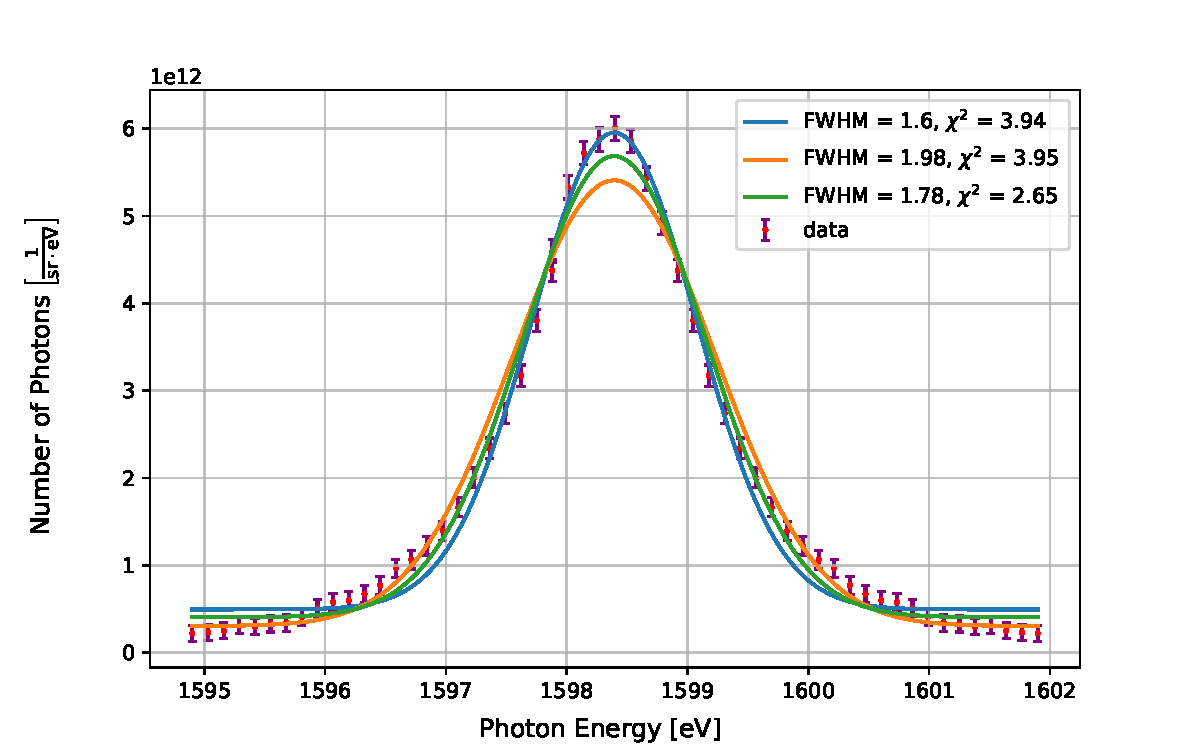
\includegraphics[width=0.9\textwidth]{Data_Analysis/resolution/peak_of_Al_(thick)_event_16_on_FSSR.pdf}
	\caption{Gaussian fit of the He-$\upalpha$ line for a \SI{24}{\joule} shot on aluminum (event 16) used to determine the spectral resolution of the FSSR. The best (green) and worst (blue and orange) fit models are depicted and labeled with their corresponding FWHM and $\chi^2$ values.}
	\label{fig: resolution FSSR}
\end{figure}

\begin{figure} [H]
	\centering
	\begin{subfigure}[t]{0.9\textwidth}
		\centering
		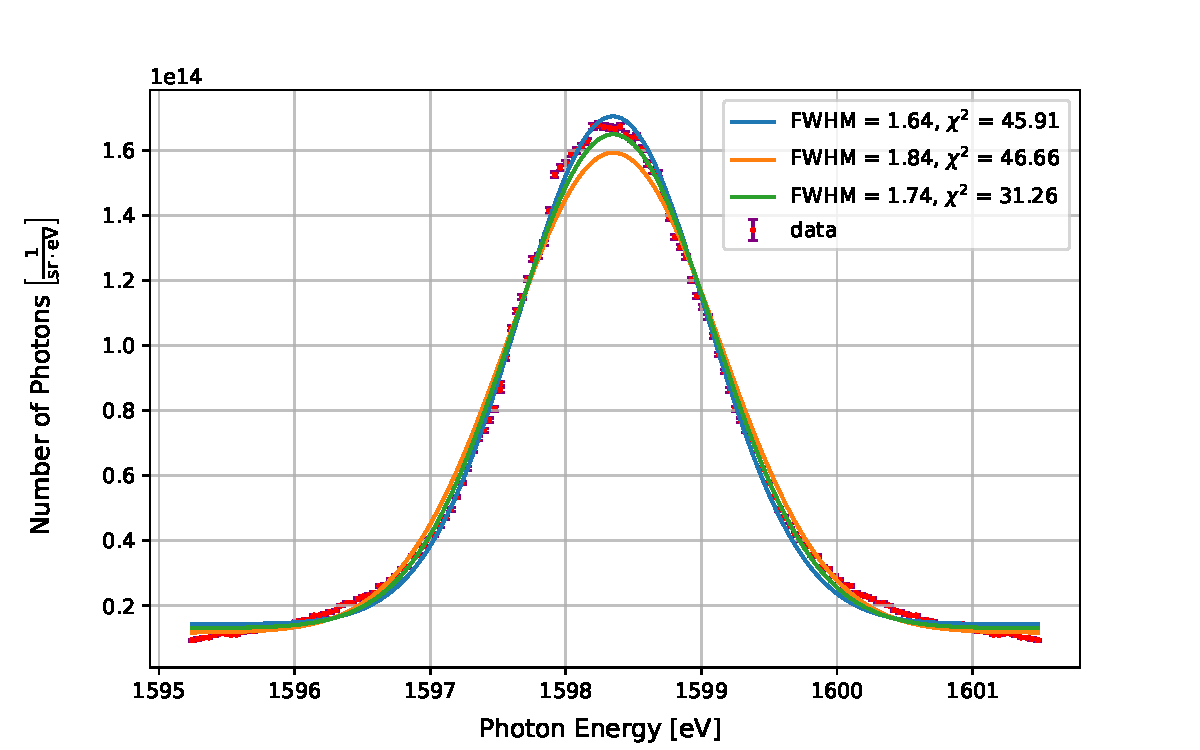
\includegraphics[width=\textwidth]{Data_Analysis/resolution/peak_of_Al_event_19_on_DUCC.pdf}
		\caption{Gaussian fit of the He-$\upalpha$ line for a \SI{27}{\joule} shot on aluminum (event 19).}
		\label{}
	\end{subfigure}%
	\hfill
	\begin{subfigure}[t]{0.9\textwidth}
		\centering
		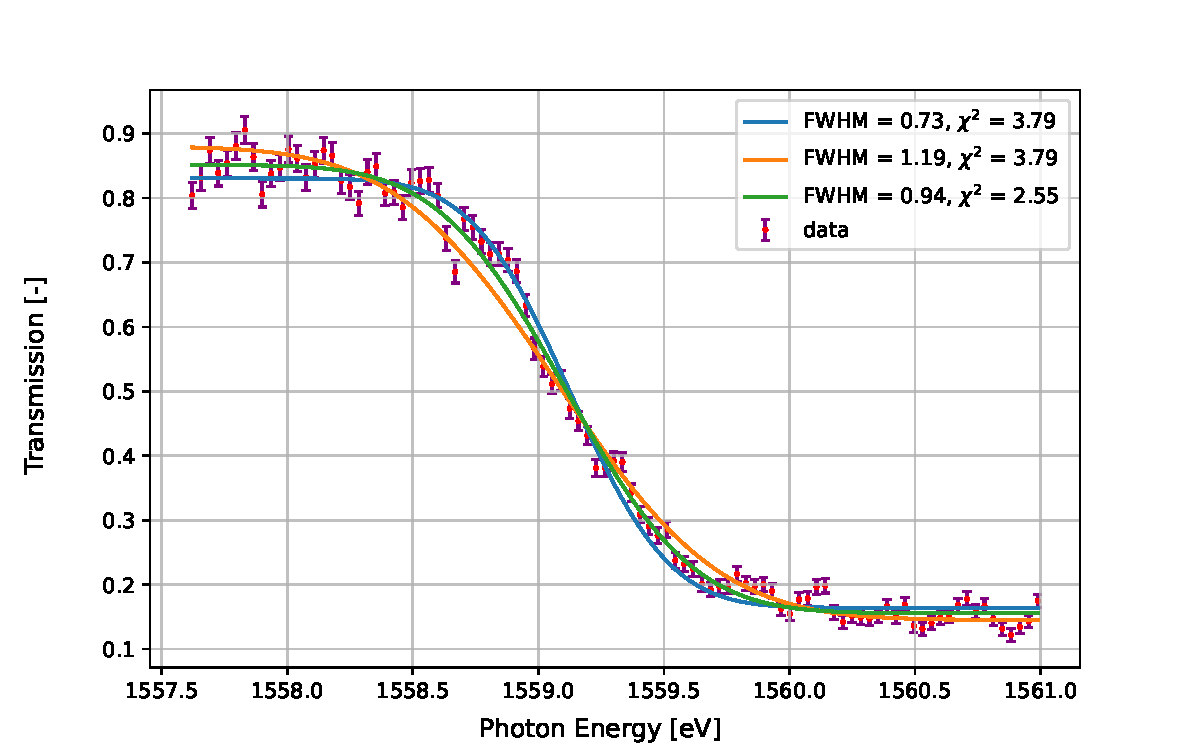
\includegraphics[width=\textwidth]{Data_Analysis/resolution/transmission_of_Gd_event_32_on_DUCC.pdf}
		\caption{Error function fit of the transmission through a \SI{1.18\pm0.12}{\milli\meter} thick aluminum sample for a \SI{87.4}{\joule} shot on gadolinium (event 32).}
		\label{}
	\end{subfigure}
	\caption{Fits used to determine the spectral resolution of the DUCC with a (a) Gaussian fit and (b) error function fit respectively. The best (green) and worst (blue and orange) fit models are depicted and labeled with their corresponding FWHM and $\chi^2$ values.}
	\label{}
\end{figure}

\begin{figure}[H]
	\centering
	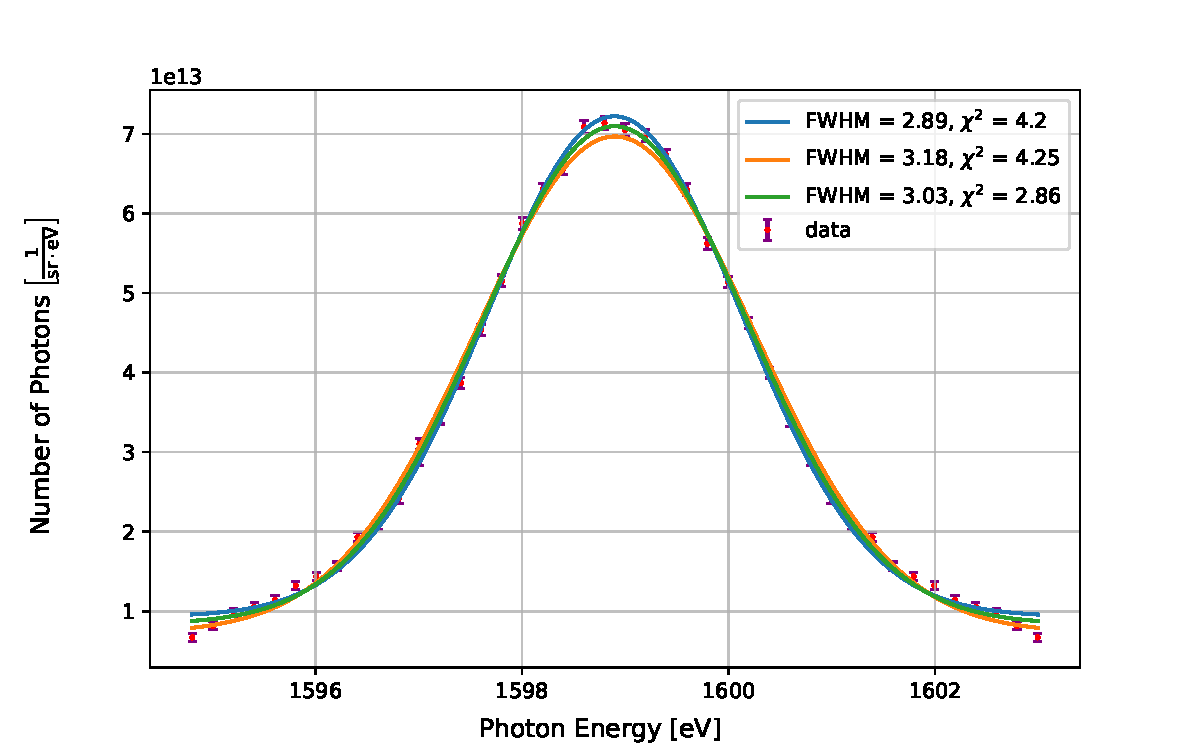
\includegraphics[width=0.9\textwidth]{Data_Analysis/resolution/peak_of_Al_event_18_on_SUCC.pdf}
	\caption{Gaussian fit of the He-$\upalpha$ line for a \SI{28}{\joule} shot on aluminum (event 18) used to determine the spectral resolution of the SUCC. The best (green) and worst (blue and orange) fit models are depicted and labeled with their corresponding FWHM and $\chi^2$ values.}
	\label{}
\end{figure}

For the SUCC and DUCC the source broadening plays a crucial role. It is derived from the source size and is influenced by the spectrometer geometry. To determine the source size, we placed a knife edge on the SUCC, consisting of an opaque metal sheet placed in front of the crystal in the x-ray path in such a way as to cover approximately half of the source image on the detector. By fitting an error function to the edge of the shadow cast by the knife edge and taking into account the magnification of the image, the FWHM of the source size in non-dispersive direction can be extracted. I then begin calculating the source broadening by projecting the source size $x_s$ onto the detector of a given spectrometer with the formula
\begin{equation}
	x_{s,d} = \frac{x_s}{\cos(\theta_0)}.
\end{equation}
The source image size $x_{s,d}$ is converted to eV using the dispersion of the spectrometer, finally resulting in the source broadening. To note is that all shots used to calculate the resolution using transmission were with a phase plate, while all the shots using the He-$\upalpha$ emission line were without a phase plate.

The Doppler broadening is from a FLYCHK simulation with the electron temperature $T_e$ = \SI{1000}{\electronvolt}, whose error is estimated from comparison to a simulation of $T_e$ = \SI{500}{\electronvolt}. In both simulations the electron density is set to \SI{4e21}{\centi\meter}$^{-3}$.

In the following I present the results for the spectral resolution calculations of the DUCC, FSSR, and SUCC. The final results for the crystal broadening as compared to the \textit{mmpxrt} simulations, adjusted according to the discussion of section \ref{section: int refl ratio}, are then given. 

The results for the DUCC shown in table \ref{Table: DUCC resolution} are calculated by neglecting the detector resolution contribution to the spectral resolution, a property that is apparent in table \ref{TableResolutions}. Interestingly, all the source sizes are larger than \SI{120}{\micro\meter} across different backlighter materials, which is expected for event 31 and 32 due to the use of a phase plate with a focus spot of at least \SI{120}{\micro\meter} in size, supporting the effectiveness of the knife edge method. Further investigation of the source sizes of a wider range of shots could be instructive for the optimization of the backlighter in future experiments. Furthermore, it is clear that the crystal broadening is the dominant contribution for the DUCC, in contrast to the theoretical predictions, where the source broadening was most significant. The higher than expected crystal broadening points to a high rocking curve width of the crystals and therefore worse crystal quality, which could be due to the fact that the ADP crystals were left exposed to air for a long period of time, as all the crystals were packaged together. The exposure could have caused absorption of water in the crystal, altering the lattice structure and crystal properties. Additionally, the crystal broadening values calculated from the transmission are in agreement, in the sense that they fall within each other's uncertainty, allowing the averaging of the two values to get $\left(0.94^{+0.31}_{-0.22}\right)$ eV. The large error range as compared to the Gaussian fit result can be attributed to the propagation of the error of two spectra, from which the transmission is determined. The crystal broadening from the transmission is more than \SI{0.6}{\electronvolt} lower than that from the Gaussian fit, a deviation that will be discussed later in this section. 

\begin{table}[H]
	\centering
	\caption{Resolution contributions of the DUCC calculated for different shots, where every value is given in eV unless another unit is expressly assigned. The results are obtained by a Gaussian fit to the Al He-a line (g) or an error function fit to the transmission (t). The detector resolution of the DUCC is negligible (see table \ref{TableResolutions}) and therefore not shown.}
	\vspace{0.05cm}
	\renewcommand{\arraystretch}{1.5}
	\centering
	\begin{tabular}{|c|c|c|c|c|c|c|c|} 
		\hline
		Event & Shot & Type & FWHM & \makecell{Source Size \\ $[$mm$]$} & \makecell{Source \\ Broadening} & \makecell{Doppler \\ Broadening} & \makecell{Crystal \\ Broadening} \\ 
		[0.5ex]
		\hline\hline
		19 & \SI{27}{\joule} on Al & g & 1.74$^{+0.11}_{-0.01}$ & 0.12$\pm$0.02 & 0.49$\pm$0.06 & 0.47$\pm$0.10 & 
		1.60$^{+0.12}_{-0.11}$ \\ 
		[0.5ex]
		\hline
		31 & \SI{92.7}{\joule} on Sm & t & 1.29$^{+0.47}_{-0.32}$ & 0.15$\pm$0.002 & 0.61$\pm$0.01 & - & 
		1.13$^{+0.53}_{-0.36}$ \\ 
		[0.5ex]
		\hline
		32 & \SI{87.4}{\joule} on Gd & t & 0.94$^{+0.25}_{-0.21}$ & 0.14$\pm$0.002 & 0.57$\pm$0.01 & - & 
		0.75$^{+0.32}_{-0.26}$ \\  
		[0.5ex]
		\hline
	\end{tabular}
	\label{Table: DUCC resolution}
\end{table}

In the case of the FSSR, the source broadening becomes negligible thanks to the focusing properties of the geometry, while the detector resolution is relevant. As displayed in table \ref{Table: FSSR resolution}, the main contribution to the spectral resolution is crystal broadening, where both shots yield approximately \SI{1.7\pm0.2}{\electronvolt}. The excellent agreement, despite the difference in laser energy of more than a factor 10, speaks for the efficacy of the analysis procedure. That the crystal broadening dominates is in agreement with theory.

\begin{table}[H]
	\centering
	\caption{Resolution contributions of the FSSR calculated for different shots, where every value is given in eV unless another unit is expressly assigned. The results are obtained by a Gaussian fit to the Al He-a line (g). The source broadening is negligible due to the focusing properties of the FSSR (see table \ref{TableResolutions}). The detector resolution uncertainty is neglected, as it is small compared to other error sources because of the precisely known pixel size.}
	\vspace{0.05cm}
	\renewcommand{\arraystretch}{1.5}
	\centering
	\begin{tabular}{|c|c|c|c|c|c|c|} 
		\hline
		Event & Shot & Type & FWHM & \makecell{Detector \\ Resolution} & \makecell{Doppler \\ Broadening} & \makecell{Crystal \\ Broadening} \\ 
		[0.5ex]
		\hline\hline
		2 & \SI{1.7}{\joule} on Al & g & 1.80$^{+0.19}_{-0.18}$ & 0.14 & 0.47$\pm$0.10 & 
		1.73$^{+0.20}_{-0.19}$ \\ 
		[0.5ex]
		\hline
		16 & \SI{24}{\joule} on Al & g & 1.78$^{+0.20}_{-0.18}$ & 0.14 & 0.47$\pm$0.10 & 
		1.71$^{+0.21}_{-0.19}$ \\ 
		[0.5ex]
		\hline
	\end{tabular}
	\label{Table: FSSR resolution}
\end{table}

For the SUCC, the detector resolution is neglected, as the spectrometer shares a basic geometry with the DUCC. In table \ref{Table: SUCC resolution} the results are presented, where again the crystal broadening dominates. Most striking is that all the crystal broadening results are in good agreement, hovering around \SI{2.4}{\electronvolt}, although the FWHM values deviate by up to \SI{0.34}{\electronvolt}, falling outside the range of the errors of the FWHM. The FWHM discrepancy is compensated by the smaller source broadening of event 16, which indicates that the source broadening processing method functions well. The overall crystal broadening agreement across shots again shows that the resolution calculation method is reliable.

\begin{table}[H]
	\centering
	\caption{Resolution contributions of the SUCC calculated for different shots, where every value is given in eV unless another unit is expressly assigned. The results are obtained by a Gaussian fit to the Al He-a line (g). The detector resolution is assumed to be negligible, following from the shared basic design of the SUCC and DUCC.}
	\vspace{0.05cm}
	\renewcommand{\arraystretch}{1.5}
	\centering
	\begin{tabular}{|c|c|c|c|c|c|c|c|} 
		\hline
		Event & Shot & Type & FWHM & \makecell{Source Size \\ $[$mm$]$} & \makecell{Source \\ Broadening} & \makecell{Doppler \\ Broadening} & \makecell{Crystal \\ Broadening} \\ 
		[0.5ex]
		\hline\hline
		16 & \SI{24}{\joule} on Al & g & 2.69$^{+0.15}_{-0.14}$ & 0.08$\pm$0.01 & 1.16$\pm$0.20 & 0.47$\pm$0.10 & 
		2.38$^{+0.20}_{-0.19}$ \\ 
		[0.5ex]
		\hline
		18 & \SI{28}{\joule} on Al & g & 3.03$^{+0.15}_{-0.14}$ & 0.11$\pm$0.03 & 1.69$\pm$0.44 & 0.47$\pm$0.10 & 
		2.48$^{+0.35}_{-0.34}$ \\ 
		[0.5ex]
		\hline
		19 & \SI{27}{\joule} on Al & g & 2.92$^{+0.19}_{-0.18}$ & 0.11$\pm$0.02 & 1.69$\pm$0.33 & 0.47$\pm$0.10 & 
		2.34$^{+0.34}_{-0.33}$ \\ 
		[0.5ex]
		\hline
	\end{tabular}
	\label{Table: SUCC resolution}
\end{table}


\begin{table}[H]
	\centering
	\caption{The final results for the experimentally determined crystal broadening compared to simulation when applicable. The results are obtained by a Gaussian fit to the Al He-a line (g) or an error function fit to the transmission (t). The experimental broadening is calculated by the mean of the crystal broadening results of all available shots.}
	\vspace{0.05cm}
	\renewcommand{\arraystretch}{1.5}
	\centering
	\begin{tabular}{|c|c|c|c|} 
		\hline
		Spectrometer & Type & \makecell{Simulated \\ Broadening} & \makecell{Experimental \\ Broadening} \\ 
		[0.5ex]
		\hline\hline
		DUCC & g &  \SI{0.24}{\electronvolt} & $\left(1.60^{+0.12}_{-0.11}\right)$ eV \\ 
		[0.5ex]
		\hline
		DUCC & t & \SI{0.24}{\electronvolt} & $\left(0.94^{+0.31}_{-0.22}\right)$ eV \\ 
		[0.5ex]
		\hline
		FSSR & g & \SI{0.54}{\electronvolt} & $\left(1.72^{+0.15}_{-0.13}\right)$ eV \\ 
		[0.5ex]
		\hline
		SUCC & g & - & $\left(2.40^{+0.18}_{-0.17}\right)$ eV \\ 
		[0.5ex]
		\hline
	\end{tabular}
	\label{Table: Final Resolutions}
\end{table}

The considerations and adjustments of section \ref{section: int refl ratio} result in the following simulated crystal broadening: \SI{0.24}{\electronvolt} for the DUCC as in the design phase and \SI{0.54}{\electronvolt} for the FSSR as calculated by the deconvolution of the spectral resolution of the new \textit{mmpxrt} simulation from the detector resolution. Table \ref{Table: Final Resolutions} compares the simulated crystal broadening to the experimentally determined ones, where it is immediately apparent that the former deviate significantly from the latter. In all cases, the main cause likely lies in the discrepancy of the rocking curve widths used in the \textit{mmpxrt} simulations (\SI{349}{\micro\radian} for mica and \SI{165}{\micro\radian} for ADP) to the real, unmeasured values. This demonstrates the inherent difficulty in assuming accurate crystal properties purely from the literature. As such, a reasonable next step would be the direct measurement of the integrated reflectivity and rocking curve width of the crystals actually used/to be used in experiments. With this information, more accurate \textit{mmpxrt} simulations could be conducted, ensuring that the desired spectral resolution is achieved in experiment. Another interesting observation is the fact that all the experimental values are higher than the simulated ones. This is expected for the FSSR, whose $\Delta \theta$ of the simulation is determined from the ray tracing code of Artem, meaning that the rocking curve width of the actual crystal is increased due to defects or damage. Despite this, the experimental crystal broadening $\left(1.72^{+0.15}_{-0.13}\right)$ eV falls well below the result in the original \textit{mmpxrt} simulation of \SI{2.95}{\electronvolt} (see table \ref{TableResolutions}), implying that the mica crystal's quality is still significantly better than that calculated by \textit{Hölzer et al.} \citep{holzer1998flat}.

Another interesting finding from table \ref{Table: Final Resolutions} is the more than 50\% deviation of the crystal broadenings found with the transmission and the He-$\upalpha$ line for the DUCC, lying outside the margins of error. A possible origin of this discrepancy is additional broadening effects of the emission line which have not been accounted for, leading to an artificially inflated result for the He-$\upalpha$ line. The most probable mechanism is Stark broadening caused by interaction with charged particles in the plasma, which broadens lines according to a Lorentz distribution. Notably, Doppler broadening dominates for high electron temperature, low electron density plasma \citep{wiese1965plasma}, as is expected for the Al plasma where He-$\upalpha$ emission is the strongest. Still, the inherent spatial and temporal inhomogeneity of laser plasma means that the influence of the Stark broadening would have to be estimated with further simulations. Another indication that could point to Stark broadening is the form of the He-$\upalpha$ line, which the Gaussian fit does not entirely correspond to, as most easily seen in fig. \ref{fig: resolution FSSR}, but also apparent for all the spectrometers. The relatively far extending wings of the data are characteristic of the Lorentz profile \citep{kunze2009introduction} and indicate that the peak likely conforms to a Voigt profile, which is the convolution of the Gauss and Lorentz profile. Despite this, a Gaussian profile is applied for the fitting because it still closely describes the data and markedly simplifies the analysis, since the Voigt fitting would require an additional fitting parameter.

To close, the experimentally determined resolutions will be compared to the requirements for EXAFS and XANES respectively. The crystal broadening for the DUCC of $\left(1.60^{+0.12}_{-0.11}\right)$ eV using the Gaussian fit method and $\left(0.94^{+0.31}_{-0.22}\right)$ from the fit of the transmission combined with the source broadening both lie above the original spectrometer design consideration for conducting XANES of $\Delta E \leq\SI{1}{\electronvolt}$. Consequently, the future use of the DUCC geometry with ADP crystals requires that the crystal properties are measured beforehand and if necessary exchanged for new crystals. Conversely, the excellent spectral resolutions, as calculated by the deconvolution of the FWHM from the Doppler broadening, of $\left(1.72^{+0.15}_{-0.13}\right)$ eV for the FSSR and $\left(2.84^{+0.10}_{-0.09}\right)$ eV for the SUCC, easily fulfill the requirement of $\Delta E <\SI{10}{\electronvolt}$ for EXAFS. As such, both the spectrometers could be considered viable candidates for future designs, purely from a spectral resolution standpoint.


\section{Setup Validation}
\label{section: setup validation}

As of yet, the spectrometers, and by extension the experimental setup have been assessed without quantitative comparison to similar experiments. To remedy this and place the captured spectra in a broader context, the conversion efficiency of the PHELIX laser energy into the He-$\upalpha$ emission line of aluminum will be extracted. I will then check the reasonableness of the results by comparing them to the expected order of magnitude estimated from the literature. A more exacting comparison is not possible in this case due to the fundamental differences between experimental setups and studied backlighter materials.

\subsection{Conversion Efficiency into He-$\upalpha$ Emission Line of Aluminum}

I determine the conversion efficiency of the laser energy into the Al He-$\upalpha$ line by first processing the source spectra of shots on aluminum as described in chapter \ref{chapter: data analysis} without the binning step, where I use the same integrated reflectivity values from the literature as in section \ref{section: int refl ratio}. I then multiply the resulting $N_{\text{st,eV}}$ in equation \ref{conversion to emitted photons} with 4$\pi$ and $\Delta E$ to get the total number of emitted photons $N_{\text{total}}$ in each energy interval covered by a given pixel. Next, I approximate integrating by summing over all the energy intervals included in the He-$\upalpha$ line, avoiding the neighboring other heliumlike ion emission line. An example of an integration area is depicted in fig. \ref{fig: CE DUCC_t}. Multiplying the energy of the line, i.e. \SI{1598.4}{\electronvolt}, onto this sum yields the total energy emitted into the He-$\upalpha$ line. The ratio of this quantity to the laser energy then gives the desired conversion efficiency.

\begin{figure}[H]
	\centering
	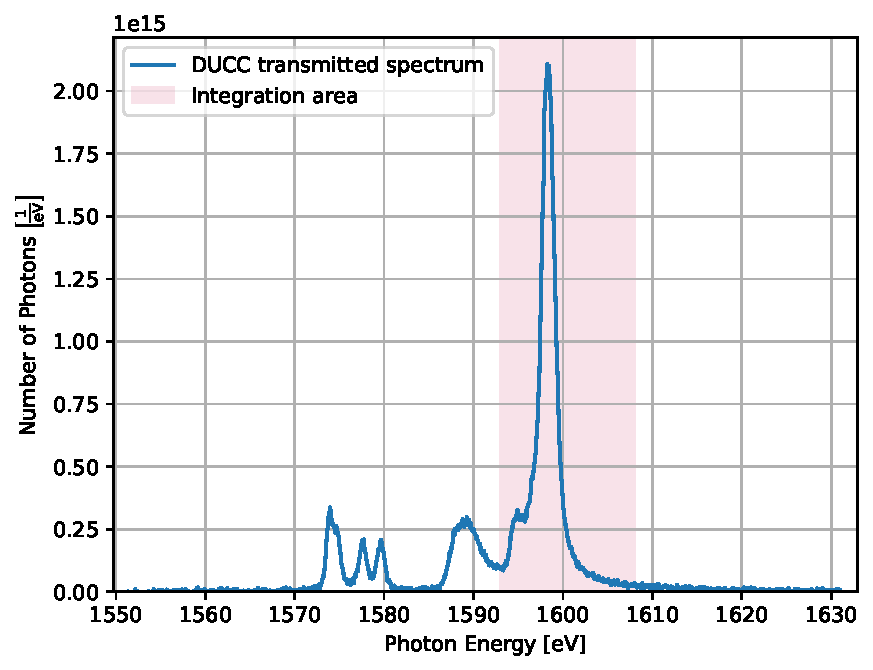
\includegraphics[width=0.8\textwidth]{Data_Analysis/converison_efficiency/spectra_of_Al_event_19_on_DUCC_transmitted_spectrum.pdf}
	\caption{Spectrum from a \SI{27}{\joule} shot on aluminum (event 19) captured with the transmission channel of the DUCC and utilized to determine the conversion efficiency. The area over which the data belonging to the Al He-$\upalpha$ line is summed is depicted in pink.}
	\label{fig: CE DUCC_t}
\end{figure}

As with the $R_{int}$ ratio, the conversion efficiency $CE$ using the FSSR can alternatively be determined through the simulated efficiency of the FSSR from section \ref{section: int refl ratio}. In this case, I use the $R_{int}$ of the mica crystal of \SI{2.752\pm0.633}{\micro\radian} derived in section \ref{section: int refl ratio} in place of the literature value and follow the same calculation as above.

In table \ref{Table: CE} I present the experimentally determined conversion efficiencies for each spectrometer, along with the integrated reflectivity used in the calculation. All the $CE$ are in the region of a few percent and lie approximately within each others error ranges, with the exception of the FSSR result derived using the literature $R_{int}$ value, again reinforcing the notion that the $R_{int}$ from simulation is closer to the actual value. This agreement also serves to demonstrate the consistency of the setup across all spectrometers and support the validity of the spectrum processing procedure.

\begin{table}[H]
	\centering
	\caption{Conversion efficiency of the laser energy into the He-$\upalpha$ line of aluminum. DUCC$_t$ refers to the transmission channel of the DUCC, DUCC$_s$ to the source channel. The integrated reflectivity value used in the calculation is given.}
	\vspace{0.05cm}
	\renewcommand{\arraystretch}{1.5}
	\centering
	\begin{tabular}{|c|c|c|c|c|} 
		\hline
		Event & Shot & Spectrometer & $R_{int}$ & \makecell{Conversion \\ Efficiency} \\ 
		[0.5ex]
		\hline\hline
		19 & \SI{27}{\joule} on Al & DUCC$_t$ & \SI{40}{\micro\radian} & (4.50$\pm$2.25)\% \\ 
		[0.5ex]
		\hline
		19 & \SI{27}{\joule} on Al & DUCC$_s$ & \SI{40}{\micro\radian} & (3.76$\pm$1.88)\% \\ 
		[0.5ex]
		\hline
		16 & \SI{24}{\joule} on Al & FSSR & \SI{53.6}{\micro\radian} & (0.20$\pm$0.10)\% \\ 
		[0.5ex]
		\hline
		16 & \SI{24}{\joule} on Al & FSSR & \SI{2.752}{\micro\radian} & (3.89$\pm$0.28)\% \\ 
		[0.5ex]
		\hline
		16 & \SI{24}{\joule} on Al & SUCC & \SI{80}{\micro\radian} & (2.55$\pm$1.28)\% \\ 
		[0.5ex]
		\hline
		19 & \SI{27}{\joule} on Al & SUCC & \SI{80}{\micro\radian} & (2.71$\pm$1.36)\% \\ 
		[0.5ex]
		\hline
	\end{tabular}
	\label{Table: CE}
\end{table}

For comparison, I estimate the expected order of magnitude for the results using values of the conversion efficiency of the Z-Beamlet laser at Sandia National Laboratories into He-like emission lines of laser-plasma of various elements ranging from Z$=21$ to 32 \citep{ruggles2003measurements}. Extrapolating from the conversion efficiencies in fig. 5 of \textit{Ruggles et. al.}'s paper, a $CE$ into the Al He-$\upalpha$ line on the order of 1\% is reasonable. Consequently, every spectrometer yields acceptable values, supporting the efficacy of the experimental setup as a whole.


	\chapter{Summary and Outlook}
\label{chapter: outlook}

In the course of this work, I designed, built, and tested two spectrometers, namely the Dual Unbent Crystal 
Spectrometer (DUCC) and the Focusing Spectrograph 
with Spatial Resolution in 1 Dimension (FSSR-1D), with the purpose of conducting XAFS on heavy-ion heated aluminum samples at GSI and FAIR. The 
DUCC aims to resolve XANES around the Al K-edge and 
leverages a dual crystal design to simultaneously 
capture a transmitted and source spectrum on 
one detector. With its flat crystal design, it emphasizes consistency and simplicity. The FSSR-1D is designed to measure 
EXAFS and sports a spherically bent crystal, which 
enables spectral focusing and 1D spatial imaging onto 
the detector, significantly reducing background and 
increasing the signal-to-noise ratio (SNR). This spectrometer prioritizes performance, having the potential for excellent spectral resolution relative to its energy range, at the cost of higher complexity and possibly lower consistency. 

The designs were informed 
by considerations stemming from the unique requirements of the experimental setup and the purpose of the spectrometers, which include: 
covering the energy ranges relevant to XANES ($\sim$1540-\SI{1585}{\electronvolt}) and 
EXAFS ($\sim$1560-\SI{1810}{\electronvolt}) respectively, limitations imposed by the WDM 
sample size ($\leq\SI{1}{\milli\meter}$) due to the uniformity requirements of the 
heavy-ion heating, goals for the spectral 
resolution for observing XANES ($\Delta E\leq\SI{1}{\electronvolt}$) and EXAFS ($\Delta E<\SI{10}{\electronvolt}$), achieving 
sufficient intensity on the detector for a workable SNR, and keeping the 
physical size ($<\SI{550}{\milli\meter}$) within the confines of the setup. In theory and simulation, both 
spectrometers fulfill all the considerations, with 
the DUCC covering an energy range of 
1541-\SI{1618}{\electronvolt}, having a sample size of 
\SI{0.75}{\milli\meter}, and exhibiting a spectrometer length of 
\SI{235.17}{\milli\meter}. The FSSR-1D records in an 
energy range of 1465-\SI{1755}{\electronvolt}, gives a 
sample size of \SI{1.07}{\milli\meter}, and has a spectrometer 
length of \SI{404.30}{\milli\meter}. The energy 
resolutions were 
determined using \textit{mmpxrt} simulations, with the exception of the crystal properties' 
contribution to the DUCC resolution determined analytically, resulting in $\Delta E = 
\SI{0.703}{\electronvolt}$ for the DUCC 
and $\Delta E = \SI{3.097}{\electronvolt}$ for 
the 
FSSR-1D. The largest contribution to $\Delta E$ originated from the source broadening for 
the DUCC using a source size of \SI{100}{\micro\meter} and the crystal properties for the FSSR-1D. With the schemes theoretically proven, the spectrometers were mechanically modeled using 
\textit{Autodesk Inventor 2020} and fabricated. Each spectrometer 
takes into account the harsh experimental conditions by 
shielding the sensitive crystals and camera chips, 
where the chips are further insulated from visible 
light, and includes necessary parts to fully 
align the spectrometers in the experimental setup, 
which must be especially exacting for the FSSR-1D.

In a laser-only experiment using the PHELIX beam conducted in May, 2023, which is part of a series of preparatory experiments for eventual WDM experiments at FAIR, I tested and vetted the DUCC and FSSR, as well as another spectrometer designed by Philipp Hesselbach called the Single Unbent Crystal Spectrometer (SUCC), whose geometry effectively corresponds to a single channel of the DUCC, adjusted to accommodate a KAP crystal instead of ADP, and is intended for capturing wide energy range (1400-\SI{1800}{\electronvolt}) source spectra as a control. The spectral data gathered as TIFF images is processed and analyzed by a \textit{python3} code I developed called \textit{AXAWOTLS}, designed from the ground up to be applicable during future beamtimes using any spectrometer. With this code, I extracted source spectra of every backlighter material, produced x-ray absorption spectra, and calculated the ratio of integrated reflectivity, the spectral resolution, and conversion efficiency of laser energy into the Al He-$\upalpha$ emission line for each spectrometer.

Every spectrometer covers the expected energy range with generally sufficient SNR, assuring that the basic geometries and designs are successful. Additionally, the x-ray source spectra behave as anticipated and yield reasonable photon numbers. In contrast, each spectrometer performs to varying degrees when extracting x-ray absorption spectra. The SUCC/OSUCC combination with a Teflon backlighter delivers absorption curves with excellent agreement with the literature, where the crystal calibration method and the smooth backlighter spectra from Teflon prove to be effective. The DUCC with rare-earth backlighters also performs well, albeit with notable features in the absorption curve due to the lack of a suitable crystal calibration shot and the requirement of rare-earth backlighters, which exhibit structure-rich source spectra. The results, along with the simplified processing, speak for the double channel design, since it enables fairly accurate absorption spectrum extraction even without crystal calibration. The same cannot be said of the SUCC/FSSR combination, which did not produce any reasonable absorption spectra. The spectrometer combination is hindered most significantly by the spectral features around the K-edge due to the mica crystal defects as well as the presence of aluminum in mica's chemical makeup, leading to an Al K-edge even in source spectra. These aspects heavily distort the fine structures around the absorption edge, making the constellation untenable for XAFS applications.

The results for the ratios of integrated reflectivity indicate that the KAP crystals of SUCC and the ADP crystals of the DUCC have comparable $R_{int}$ values, with an averaged experimental DUCC/SUCC ratio of $0.84\pm0.03$, in contrast to the literature value of 0.5. A deviation from the literature is also observed for the FSSR/SUCC ratio with an experimental value of $0.06\pm0.02$ and literature ratio of 0.67. In addition, with the help of ray tracing simulation of the FSSR conducted by Artem Martynenko, an $R_{int}$ of \SI{2.75\pm0.63}{\micro\radian} for the mica crystal was calculated, over a factor of 10 lower than the literature value of \SI{53.6}{\micro\radian} \citep{holzer1998flat} and therefore in better agreement with the experimental FSSR/SUCC ratio. These results highlight the difficulty of estimating crystal properties from the literature, since $R_{int}$ and the rocking curve width $\Delta \theta$ are highly sensitive to individual crystal quality. Accordingly, new \textit{mmpxrt} simulations were conducted for the DUCC and FSSR using adjusted crystal properties, which were estimated considering the experimental $R_{int}$ ratios and the values from Artem's simulation. The adjusted \textit{mmpxrt} simulations confirmed the validity of the original theoretical resolution of the DUCC of \SI{0.703}{\electronvolt}, while the resolution of the FSSR was reduced to \SI{0.563}{\electronvolt}, a consequence of a significantly lower mica rocking curve width. 

The adjusted theoretical resolutions proved to be universally lower than the experimentally determined ones. The crystal broadening contribution to the DUCC's spectral resolution was $\left(1.60^{+0.12}_{-0.11}\right)$ eV, as calculated from a Gaussian fit, and $\left(0.94^{+0.31}_{-0.22}\right)$ eV, as determined by an error function fit, significantly exceeding the theoretical value of \SI{0.24}{\electronvolt}. The increased crystal broadening indicates that the ADP crystals are of lower quality than expected, in terms of a higher $\Delta \theta$. Together with source broadening, the DUCC does not fulfill the resolution requirement for XANES of $\Delta E\leq\SI{1}{\electronvolt}$. In contrast, the FSSR meets the resolution requirement for EXAFS of $\Delta E <\SI{10}{\electronvolt}$ with an experimental resolution of $\left(1.72^{+0.15}_{-0.13}\right)$ eV, lower than the original simulated resolution of \SI{3.01}{\electronvolt} but higher than that of the new simulation, suggesting that the mica crystal has a lower rocking curve width than that of the literature but higher than the idealized crystal of Artem's simulation. Additionally, the SUCC is capable of EXAFS from a resolution standpoint with a resolution of $\left(2.84^{+0.10}_{-0.09}\right)$ eV.

Finally, the conversion efficiency results show good agreement between all spectrometers and fall within a reasonable order of magnitude as compared to literature, i.e. on the order of a few percent. This demonstrates that the experimental setup yields consistent measurements of the source across different spectrometers that qualitatively agree with the literature.

In light of these results, it is clear that: 
\begin{enumerate}
	\item Crystal quality plays a crucial role in the extraction of absorption spectra with resolved fine-structure, as crystal broadening significantly impacts spectrometer resolution.
	\item Smooth backlighter spectra greatly enhance the quality of the absorption spectra, since structure in the source spectra are passed on enough to be significant.
	\item Identical spectrometer channels for the transmitted and source spectra markedly improve absorption curve quality, even for structure-heavy backlighter spectra.
	\item The current ADP and mica crystals are unsuitable for this experimental setup, the former due to high crystal broadening effects, and the latter because of the aluminum in its chemical makeup, along with numerous defects.
\end{enumerate}
With these findings in mind, I recommend that the next spectrometer, which will be designed for the combined heavy-ion beam/intense laser experiment of 2024, use the double channel layout of the DUCC with KAP crystals, in combination with teflon backlighters. This design leverages the smooth spectrum of teflon with the high x-ray collection of KAP, as well as the advantages offered by the dual channels. Furthermore, the spectral resolution and energy range allows for EXAFS, as shown by the SUCC. The flat crystal design also ensures reliability and ease-of-use, which are essential when considering the high complexity of a combined experiment. Lastly, the individual features of the spectrometer have all already been proven to work, reducing the potential for unforeseen difficulties during a beamtime.

The FSSR has potential, as its resolution and inherent focusing and imaging properties, allowing for high signal-to-noise ratios, would be valuable to conducting absorption spectroscopy in volatile environments. In addition, the crystal broadening and integrated reflectivity results point to good non-local (i.e. ignoring local defects) crystal quality as compared to literature. But the advantages are counter-balanced by the presence of visible crystal damage and, more significant for this application, an inherent Al absorption edge, preventing the extraction of absorption spectra suitable for conducting EXAFS of the Al K-edge. Further research into alternative crystal materials without aluminum and additional testing of novel spectrometer designs, for example a FSSR using two spherically bent crystals, i.e. double channels, could alleviate the drawbacks of the current FSSR and leverage the focusing properties of the geometry. Even so, the time investment required, along with the further complexity introduced by such a design, make this approach difficult to realize in the scope of the currently planned experiments. Consequently, I would not recommend pursuing the FSSR design in the next combined experiments, but consider it for future experiments if resources allow. 

The DUCC geometry with ADP crystals for use with XANES should also be considered for the future, since the spectrometer fell short only in its resolution due to crystal broadening and by extension in the quality of the ADP crystals. New crystals could be ordered and tested to ensure sufficient rocking curve widths for a resolution of below \SI{1}{\electronvolt}, enabling XANES. In general, the results of this thesis highlight the importance of characterizing the crystals of a spectrometer before finalizing a design, as quality can vary significantly between individual crystals, even with shared origins. In fact, the degree to which the crystal quality effects spectrometer performance makes it sensible to stock up on and test extra crystals when possible, guaranteeing replacements in the case of unexpected damage or alterations to the crystal.

In conclusion, the careful design, realization, and detailed analysis of the spectrometers, independent 
of and in relation to the backlighters, are an important contribution to the optimization of XAFS of 
heavy-ion heated aluminum using laser-driven plasmas as x-ray sources. The recommended spectrometer design for the 2024 combined experiment and the analysis code \textit{AXAWOTLS} will simplify workflow during beamtimes and enable the extraction of high-resolution, high signal-to-noise ratio absorption spectra for EXAFS of aluminum, helping to pave the way to new WDM physics at GSI and FAIR.
	
	\newpage
	\bibliography{ThesisBib}

	\appendix
\addappheadtotoc
\renewcommand{\thechapter}{\Roman{chapter}}
\renewcommand{\thesection}{\roman{section}}

\chapter{Crystal Considerations}
\label{section: crystal}

The choice 
of crystal for the spectrometers took several 
aspects into account: 
\begin{itemize}
	\item \textbf{Lattice Spacing:} The lattice 
	spacing must lie in a range that ensures the 
	Bragg condition is fulfilled for reasonable 
	incident angles depending on the spectrometer 
	geometry and the consideration 2 outlined above. 
	\item \textbf{Diffraction Order:} Reflection 
	in the first order is preferred, as the lower 
	orders 
	typically display 
	higher reflection efficiency and cover a lower 
	energy range, corresponding to higher intensities 
	from the plasma source compared 
	to intensities at higher energies 
	\citep{monot2002high, 
	renner2019challenges}. 
	\item \textbf{Bendability:} A bent crystal 
	allows for high intensities on the detector 
	and reduces shot-to-shot fluctuations 
	\citep{levy2010double}. It could also potentially 
	offer spatial resolution. 
	\item \textbf{Intrinsic Properties:} As 
	discussed in section 2.4, a compromise between a 
	small rocking 
	curve width and sufficiently high
	integrated reflectivity is required to reach 
	high resolutions while maintaining good luminosity 
	on the detector.
	\item \textbf{Availability:} The crystals 
	themselves must be acquirable.
\end{itemize}

It is noted that various crystals were 
considered for each spectrometer, but were 
gradually eliminated during the initial 
design development. For example, KAP was 
considered for the flat 
crystal geometry, but was rejected since it 
would lead to a too 
high 
spectrometer length. Quartz also 
came into 
consideration for the FSSR-1D, but in 
the end did not allow 
for a FSSR geometry that fulfilled the 
experimental 
requirements. 

\chapter{Spectrometer Simulations}
\label{section: all simulations}

To investigate the spectrometer properties and 
validate the design I ran ray tracing 
simulations, using a self-made simple ray tracing 
code and the 
python3 ray 
tracing code mmpxrt, built by Michal 
\v{S}m\'{i}d at the Helmholtz-Zentrum 
Dresden-Rossendorf \citep{vsmid2021x}. mmpxrt is 
specialized for 
x-ray spectrometers and supports bent crystal 
geometries. 

First, I will discuss the simple ray tracing 
code and its application in section 
4.1. This is followed by the presentation and discussion of the 
results of the 
mmpxrt simulations of the DUCC and FSSR spectrometers in 
sections 4.2 and 4.3 
respectively. Finally, I will summarize the results of the 
simulations and 
present the expected contributions to the resolution for each 
spectrometer in 
section 4.4.

\section{Simple Ray Tracing of the Focusing 
Spectrograph with Spatial Resolution}
It should be noted that this code is not, strictly 
speaking, a full ray tracing program, as the 
direction and 
energy of the rays are not randomly chosen. Despite 
this I will use the term ray tracing in this section 
for simplicity.

During the design phase of this work, it was unclear how exactly 
the detector 
surface should be orientated for the FSSR-1D. In 
order to directly 
test this, I made a simple 2D ray tracing code. The 
calculation of 
the rays is 
done by finding the line equation for each ray before and after 
reflection on 
the crystal. It then uses the imaging condition in the vertical 
plane (see eq.
\ref{Sfocusing}) to find the optimal intersection point with the 
detector for 
each photon energy. The ray tracing follows the steps:
\begin{enumerate}
	\item The initial ray begins at the source, which is assumed 
	to be a point 
	source, and ends at the contact point with the crystal 
	surface. By taking 
	advantage of the known location of the source, set by the 
	geometry of the 
	spectrometer, and the circle equation of the crystal 
	curvature, the contact 
	point can be calculated for a given Bragg angle, 
	and 
	therefore energy.
	\item Using the calculated contact point and the fact that 
	the ray is 
	reflected on the crystal, the line equation of the reflected 
	ray is 
	determined. 
	\item The reflected ray is propagated until it reaches the 
	distance $b$ 
	given by the imaging condition in the vertical plane. $a$ is 
	calculated by 
	the length of the initial ray. This final point is denoted 
	as the imaging 
	point of the ray.
	\item Finally, the detector line is drawn out along the line 
	of best fit of 
	the set of imaging points for a range of energies, where all 
	rays that do 
	not land on the crystal are filtered out. 
\end{enumerate}

\begin{figure}[H]
	\centering
	\includegraphics[width=0.9\textwidth]{Diagrams/FSSRsimpleRayTracing.png}
	\caption{Simple ray tracing of the FSSR-1D with 
	a mica 
	crystal with second order diffraction, where $R = 
	155$ 
	\unit{mm}, $E_0 = 1600$ \unit{eV} and $a_0 = 
	549.7$ 
	\unit{mm}. The detector 
	length in dispersive direction is 27.6 \unit{mm} and the 
	crystal length is 
	50 \unit{mm}. The red dot represents the source 
	and the red ray is the central ray. The remaining rays are 
	shown in green 
	The crystal is in blue and the detector in black. The dotted 
	circles depict 
	the crystal curvature and the RC respectively. Finally, the 
	black dot shows 
	the center of the crystal curvature circle.}
	\label{FSSRSimpleRayTracing}
\end{figure}

The code delivers the diagram seen in fig. 
\ref{FSSRSimpleRayTracing}, where 
the parameters of the final FSSR-1D are used. 
Notably, the 
detector line 
lies exactly on a symmetry axis of the circle drawn out from the 
crystal 
curvature, even though no explicit symmetry relations were used 
in the 
calculations. This supports the optimal orientation outlined in 
section \ref{section:dispersion calculation}. In 
addition, the angle of the central ray to the detector line is 
$90\degree$, as   
expected for the FSSR-1D geometry.

To note is that this geometry has many degrees of freedom when fine tuning the 
spectrometer. As such, it's simpler to set a parameter first, then adjust the 
others accordingly. In this work, I set the central ray to be incident on the 
center of the crystal, meaning the central energy $E_0$ corresponding to this 
ray doesn't lie in the center of the energy range due to the off-axis source 
location (relative to the spherical crystal optical axis). Therefore, the 
easiest way to fine tune the energy range, limited by detector position and 
size as well as crystal position and size, is to slightly shift the detector 
location along the symmetry axis mentioned above. In this case, I chose the top 
end of the detector (positive y direction) to correspond with the topmost ray 
(lowest energy ray) reflected from the crystal, as seen in fig. 
\ref{FSSRSimpleRayTracing}. This choice covered the largest 
possible energy range with this setup. With the offset and 
orientation set, the placement of the detector is determined. 

This code is applicable for all FSSR geometries and can be used 
to quickly 
determine the optimal detector placement for any FSSR. 

\section{Simulation of the Focusing Spectrograph with 
Spatial Resolution}
\label{section: FSSR simulation}
I simulated the FSSR-1D with the same parameters as in the final 
design (see table \ref{Table: Specs}) using 
mmpxrt. In this section I will discuss the quantities relevant 
to the 
validation of the final design. For more details about each 
graph and result of 
the simulation, refer to \citep{vsmid2021x}. 

\begin{figure}[H]
	\centering
	\includegraphics[width=\textwidth]{Diagrams/FSSRmmpxrtGraphs.PNG}
	\caption{Graphical results of mmpxrt simulation 
	of the FSSR-1D, wherein the point 
		spread function used to find the energy 
		resolution is in the bottom middle.}
	\label{mmpxrtFSSRGraphs}
\end{figure}

\begin{figure} [H]
	\begin{subfigure}[t]{0.37\textwidth}
	\centering
		\includegraphics[width=\textwidth]{Diagrams/FSSRmmpxrtData.PNG}
		\caption{Numerical results of mmpxrt 
		simulation of FSSR-1D with some 
		quantities removed for clarity.}
		\label{mmpxrtFSSRData}
	\end{subfigure}%
	\hfill
	\begin{subfigure}[t]{0.68\textwidth}
	\centering
		\includegraphics[width=\textwidth]{Diagrams/DispersionComparisonFSSR.png}
		\caption{Dispersion of the FSSR-1D calculated 
		with three 
		different methods.}
		\label{DispComparisonFSSR}
	\end{subfigure}%
	\caption{(a): Results of simulation of 
	the FSSR-1D with the parameters as in 
	fig. \ref{FSSRSimpleRayTracing}. Simulated using 
	mmpxrt \citep{vsmid2021x}. (b): Comparison of 
	dispersion. Energy range was extended for the 
	simple ray tracing and analytical results to 
	render them visible on the graph. }
	\label{mmpxrtFSSR}
\end{figure}

To run the ray tracing simulation, a number of parameters needed 
to be input. 
These include the geometry dependent parameters like radius of 
crystal 
curvature and source-crystal distance, among others, along with 
settings 
pertaining to the simulation and source/crystal 
properties. I set the simulation settings according 
to limitations 
of the computer 
and code, where the most important is the parameter 
p['simulation']['numerical\_intersect\_halving']=1, which 
increases the runtime 
but is necessary for simulating curved crystals. As for the 
source and crystal 
properties, I set the source to be a cube with length of 0.1 
\unit{mm} and the 
crystal as a monocrystal with a rocking curve width of 
\SI{2322}{\micro\radian}
and an integrated reflectivity of 
\SI{28.9}{\micro\radian}, as typical values for mica
\citep{holzer1998flat}.



To assess the accuracy of the simulation, I will first 
look at the dispersion. I determined the dispersion using three 
different 
techniques and graphed them together in fig. 
\ref{DispComparisonFSSR}. The 
simple ray tracing calculation was done by finding $d$ through 
the absolute 
distance between the imaging points of a given ray and the 
central ray. This is 
an excellent approximation, as the detector line 
follows the line of 
imaging points 
almost exactly, with negligibly small deviations on 
the order of 
$10^{-13}$\,\si{\milli\meter}. 
For the analytical calculation I used the relation in eq. 
\ref{DispersionCalcFSSR}. The simulation dispersion is found in 
fig. 
\ref{mmpxrtFSSRData}, where one need only take the 
inverse. It's 
immediately clear 
that the results show extremely good agreement. In fact, the 
lines overlap 
almost perfectly. This speaks for the validity of all three 
methods. 
Furthermore, the dispersion is, as desired, approximately 
linear over the energy range covered by the detector, 
as apparent 
in the fit of the analytical formula 
\begin{equation}
d(E) = 1.932\cdot 
10^{-5}\,\si{\milli\meter\per\electronvolt\squared} \cdot E^2 
+ 0.03292\,\si{\milli\meter\per\electronvolt} \cdot E - 102.1 
\,\si{\milli\meter} + \mathcal{O}(E^3).
\end{equation}

The simulation recovers an energy range of 1465 - 
1757\,\si{\electronvolt}, 
which is comparable to the range expected from the FSSR-1D 
design of 
approximately 1465 - 1755\,\si{\electronvolt}. Additionally, the 
dispersion per pixel, using a pixel size of 
\SI{13.5}{\micro\meter}, is 
reasonable when 
compared to the estimated value of \SI{0.14}{\electronvolt\per 
pixel} from the 
analytical 
formula. The magnification in dispersive direction 
and source size broadening 
are also as 
expected, taking negligibly small values, with the 
source broadening resulting in $\Delta E = 
$\SI{0.014}{\electronvolt}, assuming a source size of 
\SI{150}{\micro\meter}.

Before discussing the energy resolution, an 
explanation of each type of resolution given in the 
mmpxrt results is useful (see fig. 
\ref{mmpxrtFSSRData}). Each of the three resolutions 
given is derived from the point spread function (PSF) 
seen in fig. \ref{mmpxrtFSSRGraphs} using different 
methods. The first value from "vertical spread from 
rms" is calculated by taking the root-mean-square of 
the spread of points in the d direction, then 
multiplying a factor onto it to approximate a 
gaussian profile. Consequently, this value is not of 
much immediate use in this work, as it assumes a 
distribution. The second value from "vertical spread 
from fwhm" corresponds to the FWHM of the plot of the 
profile in dispersive (d) direction, integrating over 
the y direction. As such, this resolution takes into 
account the full y range shown in the PSF graph. The 
third value from "vert. spr. narrow (fwhm) uses the 
same process as the second value, with the exception 
of using only the y range shown by two red lines in 
the PSF graph. In summary, the first value will not 
be used in this work, while the choice between the 
second and third value depends on the y range on the 
detector one wishes to cover. It is important to 
mention that this energy resolution result takes only 
the crystal quality into account.

In the case of the FSSR-1D, the most instructive 
energy resolution is the second one, as the detector 
is large enough in the vertical direction 
(\SI{6.9}{\milli\meter}) to capture all the rays in 
the PSF graph. The result $\Delta E = 
2.954$\,\si{\electronvolt} is comparable to an 
estimated value of $\Delta E_{est} = 
2.960$\,\si{\electronvolt}, calculated from the 
rocking curve width $\Delta\theta =$ 
\SI{2322}{\micro\radian} with the formula
\begin{equation}
	\Delta E_{est} = E(\theta_0) - E(\theta_0 + 
	\Delta\theta),
	\label{eq: energy resolution estimate}
\end{equation}
where $E(\theta)$ is determined using Bragg's law 
(see eq. \ref{Bragg}). The agreement between the 
estimated and simulated value speaks for the 
trustworthiness of the result. To note is that this 
energy resolution depends directly on the crystal 
quality, and 
as such can be noticeably different in the experiment.

\section{Simulation of the Dual Unbent Crystal 
Spectrometer}
\label{section: DUCC Simulation}
As with the FSSR-1D, I simulated the DUCC using the 
parameters as 
in the design (see section \ref{section:DUCC 
design}), where only one 
channel was 
considered, as the geometry is analogous along both channels. 

The source and simulation parameters in mmpxrt were set just as 
in section \ref{section: FSSR simulation}, 
with the exception of leaving out the 
"numerical\_intersect\_halving" parameter, 
since the crystal is flat. The geometry parameters were chosen 
as in the actual 
design (see table \ref{Table: Specs}). The crystal 
properties were chosen to 
correspond to a 
monocrystal with an integrated 
reflectivity 
of \SI{2.32}{\micro\radian}, taken from 
\citep{ferrari2019characterization}, and 
rocking curve width of \SI{800}{\micro\radian}, which 
was artificially increased from the literature value 
of 
\SI{165}{\micro\radian} \citep{rajesh2015growth}, since the 
simulation did not 
function for too small a $\Delta \theta$, most likely owing to 
too few 
reflected rays.


\begin{figure}[H]
	\centering
	\includegraphics[width=\textwidth]{Diagrams/DUCCmmpxrtGraphs.PNG}
	\caption{Graphical results of mmpxrt simulation 
	of the DUCC, wherein the point 
		spread function used to find the energy 
		resolution is in the bottom middle.}
	\label{mmpxrtDUCCGraphs}
\end{figure}

\begin{figure} [H]
	\begin{subfigure}[t]{0.37\textwidth}
	\centering
		\includegraphics[width=\textwidth]{Diagrams/DUCCmmpxrtData.PNG}
		\caption{Numerical results of mmpxrt 
		simulation of DUCC with some 
		quantities removed for clarity.}
		\label{mmpxrtDUCCData}
	\end{subfigure}%
	\hfill
	\begin{subfigure}[t]{0.68\textwidth}
	\centering
		\includegraphics[width=\textwidth]{Diagrams/DispersionComparisonDUCK.png}
		\caption{Dispersion of the DUCC calculated 
		with two different methods.}
		\label{DispComparisonDUCK}
	\end{subfigure}%
	\caption{(a): Results of simulation of 
	the DUCC with the parameters as in 
	table \ref{Table: Specs}. Simulated using 
	mmpxrt \citep{vsmid2021x}. (b): Comparison of 
	dispersion calculated analytically and 
	through the mmpxrt simulation.}
	\label{mmpxrtDUCC}
\end{figure}

As before, the dispersion $d(E)$ is determined using different 
methods, namely 
by the simulation and analytically using eq. 
\ref{DispersionCalcDUCK}. The 
results are pictured in fig. \ref{DispComparisonDUCK}, where 
again a very good 
agreement is apparent. In this case the dispersion is also 
approximately 
linear, albeit less than for the FSSR-1D, with a fit 
of the 
analytical 
equation resulting in 
\begin{equation}
d(E) = 6.306\cdot 
10^{-4}\,\si{\milli\meter\per\electronvolt\squared} \cdot E^2 
-2.35\,\si{\milli\meter\per\electronvolt} \cdot E - 2139 
\,\si{\milli\meter} + \mathcal{O}(E^3).
\end{equation}

The energy range as well shows good agreement, with ranges of 
1541 - 
1618\,\si{\electronvolt} for the simulation and approximately 
1541 - 
1620\,\si{\electronvolt} for the design. The dispersion per 
pixel is also as 
expected, with 0.037\,\si{\electronvolt\per pixel} for the 
analytical 
dispersion taking into account the pixel size of 
\SI{13.5}{\micro\meter}, which 
is low 
enough to display as 0.0\,\si{\electronvolt\per pixel} in the 
simulation.

In the case of the source broadening, the 
simulation results slightly deviate from the 
analytically 
estimated value. This estimate assumes a 
source size in 
the dispersive plane of \SI{150}{\micro\meter} and 
uses 1-to-1 imaging of a 2D source onto the detector, 
which follows from the 
geometry and the fact that source extension in the 
vertical direction should not affect spectral 
resolution. Together with the dispersion, this 
delivers a broadening of \SI{0.592}{eV}, while the 
simulation gives a value of 
$\SI{4.14}{\electronvolt\per\milli\meter}\cdot 
\SI{0.15}{\milli\meter} = \SI{0.621}{\electronvolt}$. 
The deviation can be possibly traced back to 
the way that mmpxrt handles the source broadening 
calculation, which is done using a monochromatic ray 
tracing, where an offset of the source is 
introduced for some rays \citep{vsmid2021x}. 
Accordingly, the source broadening becomes dependent 
on the crystal quality. The artificially increased 
rocking curve width therefore leads to higher values 
of the source broadening in the code. Despite this, 
the simulation value will be carried over, as the 
estimate is fairly coarse.

For the energy resolution, as opposed to the FSSR-1D, 
the third value in fig. \ref{mmpxrtDUCCData} is used, 
as the detector only covers a fraction of the y range 
in the PSF graph, so that $\Delta E = 
$\SI{0.952}{\electronvolt}, while the formula to 
estimate the spectral resolution from the rocking 
curve width (see eq. \ref{eq: energy resolution 
estimate}) yields $\Delta E_{est} = 
$\SI{0.238}{\electronvolt}. Due to the artificial 
increase of $\Delta\theta$ in the simulation, $\Delta 
E_{est}$ will be used instead of $\Delta E$ in this 
work.


\section{Summary of Simulation Results}
\label{section: simulation results}
For both the DUCC and FSSR-1D spectrometers, the mmpxrt 
simulations yielded 
results consistent with the analytical calculations, 
showing very good 
agreement for the 
dispersion, dispersion per pixel and energy range, 
and good agreement for source broadening. The 
energy resolution agreed well for the FSSR-1D, while 
the $\Delta E_{crystal}$ from the DUCC simulation is 
not 
meaningful due to the artificially increased 
$\Delta\theta$.

Since one of the main goals of the simulations was assessing the 
spectral 
resolution of each spectrometer, I have gathered and presented 
the 
contributions to the resolutions in table 
\ref{TableResolutions}, along with the total spectral 
resolution $\Delta E_{tot}$ calculated by summing all 
the results. 

It is immediately clear that the crystal properties 
are the main limiting factor on the resolution for 
the FSSR-1D, while the DUCC resolution is mostly 
limited 
by the source broadening, with a significant, though 
smaller, contribution from the rocking curve width. 
Here we see the advantage offered by the ADP crystal 
in comparison to the mica, in that it delivers better 
spectral resolution, albeit at the cost of lower 
integrated reflectivity and worse bendability. These 
results also indicate that the detector 
resolution does not limit the overall spectral 
resolution for either spectrometer. In general, both 
spectrometers have sufficient 
spectral resolutions to perform their roles outlined 
in section \ref{section: spectrometer geometries}.

\begin{table}[H]
\centering
\caption{Resolution contributions for the DUCC and FSSR-1D 
spectrometers. 
 In both cases, the source broadening is taken from 
 mmpxrt and assumes a source size of 
 \SI{150}{\micro\meter}, and the detector resolution 
 is calculated from the mmpxrt dispersion and uses a 
 pixel size of \SI{13.5}{\micro\meter}. The 
 contribution due to the crystal properties for the 
 DUCC is estimated as described in section 
 \ref{section: DUCC Simulation}, while for the 
 FSSR-1D it is taken from mmpxrt's second $\Delta E$ 
 value. The total spectral resolution is calculated by using error propagation 
 on the source broadening and crystal properties' resolution, then linearly 
 adding on the detector resolution.}
\vspace{0.05cm}
\renewcommand{\arraystretch}{1.5}
\centering
\begin{tabular}{|c|c|c|} 
\hline
$\Delta E$ Contributions & DUCC 
& FSSR-1D \\ [0.5ex]
\hline\hline
Source Broadening & \eV{0.621} & \eV{0.014} \\ 
[0.5ex]
\hline
Detector & \eV{0.038} & \eV{0.143} \\ [0.5ex]
\hline
Crystal Properties & \eV{0.238} & \eV{2.954} \\ 
[0.5ex]
\hlineB{7}
Total & \eV{0.703} & \eV{3.097} \\ [0.5ex]
\hline
\end{tabular}
\label{TableResolutions appendix}
\end{table}

\chapter{Alignment Procedure for FSSR-1D}
\label{section: FSSR-1D alignment}

The alignment process can be broken down into 5 steps. To note is that parts of 
the alignment are built into the mechanical design itself, such that manual 
adjustments are not required. I will touch on these aspects after explaining 
the procedure. 

Essential to the alignment are the four optical stages labeled in fig. 
\ref{InvFSSRAlignment}. The rotation stage is a PR01/M, the large 
linear stage a LX10/M, and the tip-tilt stage a KM100B/M from 
\textit{Thorlabs}. The fine linear stage, a TSDS-1 from 
\textit{SigmaKoki}, serves to adjust the crystal-pin distance and the 
tip-tilt stage allows for pointing in step 2. 

The first three steps are conducted outside the target chamber on an optical 
table equipped with an expanded collimated laser beam, in our case a 
HeNe laser, while the last two steps are carried out in 
the chamber.

\begin{enumerate}
	\item First, the FSSR-1D without the crystal apparatus is brought into 
	alignment with the HeNe beam for the next steps, simultaneously ensuring 
	that the spectrometer 
	base plate lies parallel to the floor. The HeNe beam is directed onto the 
	opening of the front plate, onto which a pin is affixed, as seen in 
	fig \ref{InvFSSRAlignment11}. The shadow cast by the pin is then 
	aligned with the center of 
	the cross on a plate attached to the back of the base of the 
	FSSR-1D (see fig. \ref{InvFSSRAlignment12}). In this way the beam 
	is parallel to the base plate of the FSSR-1D and to the line drawn 
	out from the pin to the rotation axis of the rotation stage.
	\item Now the crystal apparatus, consisting of the rotation stage, 
	fine linear stage, tip-tilt stage and the crystal holder, is put 
	in, as seen in fig. \ref{InvFSSRAlignment21}. Using the fine linear 
	stage and tip-tilt stage, the beam is 
	focused with the crystal onto the 
	surface of the pin (see fig. \ref{InvFSSRAlignment22}), whose 
	distance to the crystal is exactly the 
	focal length of the crystal. This 
	serves to set the location of the Rowland circle 
	and ensure that the crystal center intersects the rotation axis of 
	the rotation stage. It also corrects for any unintended tilts or 
	shifts of the crystal w.r.t the rest of the spectrometer. 
	\item Next, the central Bragg angle is set by rotating the crystal 
	with the rotation stage. This step leaves the crystal in its final 
	position (see fig. \ref{InvFSSR}). In preparation for the next 
	step, the pin is removed 
	and the pointer holder shown in fig. \ref{InvFSSRAlignment3} is 
	attached to the front of the front plate. Analogously to the DUCC, 
	an optical post is set to the required distance and screwed onto 
	the pointer holder.
	\item The pointer is then used to orientate the FSSR-1D in the 
	chamber. This is equivalent to fixing the $a_0$ 
	distance as defined in section \ref{SectionTheoryFSSR}.
	\item Finally, a laser is shone onto the tip of a needle placed at 
	the TCC. This 
	allows for taking images of the source with photons in the optical 
	range being reflected on the crystal and detected by the CCD camera 
	of the FSSR-1D. By adjusting the distance from chip to 
	crystal using the large linear stage under the camera pictured in 
	fig. \ref{InvFSSRAlignment12}, the position of best focus is found, 
	resulting in the thinnest possible horizontal line on the camera. 
	This is paramount to setting the 
	$b_0$ distance for the FSSR-1D geometry.
\end{enumerate}

With this the alignment is complete and the FSSR-1D geometry is realized. The 
most important mechanical details that assist in the alignment are as follows:
\begin{itemize}
	\item The rotation stage, front plate, cross plate (used in the first step) 
	and camera linear stage all lie in grooves in the base plate, which fixes 
	their locations and angles w.r.t one another. 
	\item Through additional positioning grooves for the pin and pointer 
	holder, the relative distances between every part is further preserved by 
	mechanical precision. In this way the distance from pin to rotation axis of 
	the rotation stage is set to the focal length of the spherical crystal, 
	allowing the second alignment step to line up the crystal center with the 
	rotation axis. 
	\item Finally, the crystal holder and corresponding connections to the 
	stages ensure that the crystal lies at the correct height and parallel to 
	the base plate, carrying over the alignment achieved in the first step. 
\end{itemize}

With this setup the error of the alignment is mostly limited to mechanical 
precision, excepting the fourth step, which relies on bare-eye precision. 
Despite this the overall precision remains excellent, as this uncertainty 
occurs relatively far from the spectrometer itself, reducing its 
impact.  

\begin{figure}[H]
	\centering
	\includegraphics[width=0.4\textwidth]{InventorPics/Alignment3.PNG}
	\caption{Front view of step 3 depicting the pointer 
		holder set in 
		its groove in purple.}
	\label{InvFSSRAlignment3}
\end{figure}

\begin{figure} [H]
	\centering
	\begin{subfigure}[t]{0.42\textwidth}
		\includegraphics[width=\textwidth]{InventorPics/Alignment1.1.PNG}
		\caption{Top view of step 1. The HeNe beam is directed through 
		the front plate opening onto the cross plate.}
		\label{InvFSSRAlignment11}
	\end{subfigure}%
	\hfill
	\begin{subfigure}[t]{0.56\textwidth}
	\centering
		\includegraphics[width=\textwidth]{InventorPics/Alignment1.2.PNG}
		\caption{Back view of step 1, where the shadow of the pin is 
		visible in the HeNe beam. The rotation stage and large linear 
		stage are labeled.}
		\label{InvFSSRAlignment12}
	\end{subfigure}\\[1ex]
	\centering
	\begin{subfigure}[t]{0.48\textwidth}
	\centering
		\includegraphics[width=\textwidth]{InventorPics/Alignment2.1.PNG}
		\caption{Front view of focusing in step 2. The focused HeNe 
		beam is depicted within the main beam in a darker red. The 
		rotation axis of the rotation stage is also shown.}
		\label{InvFSSRAlignment21}
	\end{subfigure}% 
	\hfill
	\begin{subfigure}[t]{0.48\textwidth}
	\centering
		\includegraphics[width=\textwidth]{InventorPics/Alignment2.2.PNG}
		\caption{Back view of focusing in step 2. The tip-tilt and fine 
		linear stage are labeled.}
		\label{InvFSSRAlignment22}
	\end{subfigure}
	\caption{Model depicting the alignment process for the FSSR-1D 
	using a collimated HeNe laser, which is shown in red. The various 
	optical stages are labeled.}
	\label{InvFSSRAlignment}
\end{figure}

\chapter{Supplementary Results}
\label{appendix: supplementary results}


\section{Spectral Resolution}
\label{appendix: spectral resolution}

\begin{figure} [H]
	\centering
	\begin{subfigure}[t]{0.49\textwidth}
		\centering
		\includegraphics[width=\textwidth]{Data_Analysis/resolution/peak_of_Al_event_2_on_FSSR.pdf}
		\caption{FSSR: Gaussian fit of the He-$\upalpha$ line for a \SI{1.7}{\joule} shot on aluminum (event 2).}
		\label{}
	\end{subfigure}%
	\hfill
	\begin{subfigure}[t]{0.49\textwidth}
		\centering
		\includegraphics[width=\textwidth]{Data_Analysis/resolution/peak_of_Al_(thick)_event_16_on_SUCC.pdf}
		\caption{SUCC: Gaussian fit of the He-$\upalpha$ line for a \SI{24}{\joule} shot on aluminum (event 16).}
		\label{}
	\end{subfigure}
	\begin{subfigure}[t]{0.49\textwidth}
		\centering
		\includegraphics[width=\textwidth]{Data_Analysis/resolution/transmission_of_Sm_event_31_on_DUCC.pdf}
		\caption{DUCC: Error function fit of the transmission for a \SI{92.7}{\joule} shot on samarium (event 31).}
		\label{}
	\end{subfigure}%
	\hfill
	\begin{subfigure}[t]{0.49\textwidth}
		\centering
		\includegraphics[width=\textwidth]{Data_Analysis/resolution/peak_of_Al_event_19_on_SUCC.pdf}
		\caption{SUCC: Gaussian fit of the He-$\upalpha$ line for a \SI{27}{\joule} shot on aluminum (event 19).}
		\label{}
	\end{subfigure}
	\caption{Fits used to determine the spectral resolution of various spectrometers. The best (green) and worst (blue and orange) fit models are depicted and labeled with their corresponding FWHM and $\chi^2$ values.}
	\label{}
\end{figure}

\section{Integrated Reflectivity Ratio}
\label{appendix: integrated reflectivity ratio}

\begin{figure}[H]
	\centering
	\includegraphics[width=0.6\textwidth]{Data_Analysis/R_int_ratio/spectra_of_Al_event_19_source.pdf}
	\caption{$R_{int}\cdot N_{total}$ for a \SI{27}{\joule} shot on aluminum (event 19). The spectra from the source channel of the DUCC and the SUCC are presented, as well as the integration area used to calculate the integrated reflectivity ratio.}
	\label{}
\end{figure}

\begin{figure}[H]
	\centering
	\includegraphics[width=0.6\textwidth]{Data_Analysis/R_int_ratio/spectra_of_Al_(thick)_event_16.pdf}
	\caption{$R_{int}\cdot N_{total}$ for a \SI{24}{\joule} shot on aluminum (event 16). The spectra from the FSSR and the SUCC are presented, as well as the integration area used to calculate the integrated reflectivity ratio.}
	\label{}
\end{figure}

\section{Conversion Efficiency into He-$\upalpha$ Emission Line of Aluminum}

\begin{figure} [H]
	\centering
	\begin{subfigure}[t]{0.49\textwidth}
		\centering
		\includegraphics[width=\textwidth]{Data_Analysis/converison_efficiency/spectra_of_Al_event_19_on_DUCC_source_spectrum.pdf}
		\caption{DUCC source channel: Spectrum from a \SI{27}{\joule} shot on aluminum (event 19).}
		\label{}
	\end{subfigure}%
	\hfill
	\begin{subfigure}[t]{0.49\textwidth}
		\centering
		\includegraphics[width=\textwidth]{Data_Analysis/converison_efficiency/spectra_of_Al_(thick)_event_16_on_SUCC.pdf}
		\caption{SUCC: Spectrum from a \SI{24}{\joule} shot on aluminum (event 16).}
		\label{}
	\end{subfigure}
	\begin{subfigure}[t]{0.49\textwidth}
		\centering
		\includegraphics[width=\textwidth]{Data_Analysis/converison_efficiency/spectra_of_Al_event_19_on_SUCC.pdf}
		\caption{SUCC: Spectrum from a \SI{27}{\joule} shot on aluminum (event 19).}
		\label{}
	\end{subfigure}%
	\hfill
	\begin{subfigure}[t]{0.49\textwidth}
		\centering
		\includegraphics[width=\textwidth]{Data_Analysis/converison_efficiency/spectra_of_Al_(thick)_event_16_on_FSSR.pdf}
		\caption{FSSR: Spectrum from a \SI{24}{\joule} shot on aluminum (event 16).}
		\label{}
	\end{subfigure}%
	\caption{Spectra from various spectrometers utilized to determine the conversion efficiency. The area over which the signals belonging to the Al He-$\upalpha$ line are summed is depicted in pink.}
	\label{}
\end{figure}

\section{Additional Simulations}
\label{section: new simulations}

\begin{figure}[H]
	\centering
	\includegraphics[width=1.12\textwidth, angle=90]{Data_Analysis/mmpxrt_DUCC_new_values.png}
	\caption{Results of \textit{mmpxrt} simulation of the DUCC with an integrated reflectivity of \SI{40}{\micro\radian} and a rocking curve width of \SI{165}{\micro\radian}}
	\label{fig: DUCC new mmpxrt}
\end{figure}

\begin{figure}[H]
	\centering
	\includegraphics[width=1.15\textwidth, angle=90]{Data_Analysis/mmpxrt_FSSR_new_values.png}
	\caption{Results of \textit{mmpxrt} simulation of the FSSR with an integrated reflectivity of \SI{2.752}{\micro\radian} and a rocking curve width of \SI{349}{\micro\radian}, as derived by Artem's simulation.}
	\label{fig: FSSR new mmpxrt}
\end{figure}

\chapter{Uncertainty Analysis}
\label{chapter: uncertainty analysis}

In this chapter, the error calculations for the quantitative results presented in chapter \ref{chapter: results and discussion} are elaborated on. As section \ref{section: qualitative performance} contains solely qualitative results, only the results of the remaining sections, namely \ref{section: spectrometer characterization} and \ref{section: setup validation}, will be addressed. 

Every error calculation begins with the statistical error, which consists of camera background noise and Poisson noise. I compute the background noise by first getting the standard deviation of the signals of every pixel in the area of the TIFF image from which the background is extracted, e.g. the middle region in fig. \ref{fig: analysis overview}. In the case of the SUCC and DUCC, this standard deviation is then divided by the number of pixel rows $N_{rows}$ that is used for the horizontal lineout of the source spectrum to account for the averaging. For the FSSR, the final background noise corresponds to standard deviation times $\sqrt{N_{rows}}$, since the lineout is formed with summing.

The Poisson noise calculation begins with the raw spectrum extracted by the first part of \textit{AXAWOTLS}, i.e. the counts for each photon energy. As the Poisson noise accounts for the full counts on the ccd chip, for the DUCC and SUCC I multiply $N_{rows}$ onto the raw spectrum counts to approximately undo the averaging of the lineout. The FSSR spectrum is left the same. I then apply equation \ref{eq: detector correction} to get the number of photons incident on the ccd chip. The square root of this number yields the Poisson noise in photons. Inserting this result in the inverse of equation \ref{eq: detector correction} gives the counts noise, which for the DUCC and SUCC is divided by $N_{rows}$ to reinstate the lineout averaging. The sum of the Poisson noise and camera background noise gives the statistical error in counts. As the rest of the spectrum processing steps consist of linear calculations, the statistical error can be propagated just like a standard spectrum, effectively converting it to number of photons per steradian per eV.

For every result, a flat error of 20\% of the mean signal of the peak is imposed on the FSSR, which is added onto the statistical error to account for the poor crystal quality.

\section{Spectral Resolution}

The uncertainty of the FWHM of the fits takes the error of the data points into consideration by nature of the algorithm outlined in section \ref{subsection: spectral resolution}. In this case the only error present on the data is the statistical error. For the cases using the transmission data, the error of both source and transmitted spectra are extended using Gaussian error propagation. The remaining uncertainties of the resolution contributions are determined as follows:
\begin{itemize}
	\item Source broadening: The error of the source size found from the fitting of the knife edge image is carried over to the source broadening through the same path at the source size, since the relations are linear.
	\item Doppler broadening: FLYCHK simulations of Al plasma with an electron temperature of $T_e$ = \SI{1000}{\electronvolt} deliver the base broadening of \SI{0.474}{\electronvolt}. The difference of this value and the Doppler broadening of the He-$\upalpha$ line for $T_e$ = \SI{500}{\electronvolt} corresponds to the error.
	\item Crystal broadening: Gaussian error propagation is applied to equation \ref{eq: crystal broadening}, giving
	\begin{equation}
		s_{crystal} = \frac{1}{\sigma_{crystal}}\sqrt{\text{FWHM}^2\cdot s_{\text{FWHM}}^2 + \sum_{i} \sigma_i^2\cdot s_i^2},
	\end{equation}
	where $s$ represents the uncertainty of each resolution contribution.
\end{itemize}

\section{Ratio of Integrated Reflectivities}

The error on the data points is a combination of the statistical error and a systematic error in the form of a filter transmission error. The latter is based off a 5\% uncertainty placed on the filter thickness. This relative error is propagated to the filter transmission, which is converted into an absolute error on the counts. The sum of this error and the statistical error builds the uncertainty on the signal. In addition, a systematic error of \SI{5}{\milli\meter} is imposed on the diverging distance and added onto the cumulative error. Through Gaussian error propagation, the error is passed onto the final $R_{int}$ ratio. The same method is applied for the $R_{int}$ of the FSSR computed using the simulated efficiency.

\section{Conversion Efficiency into He-$\upalpha$ Emission Line of Aluminum}

The uncertainty of $CE$ is determined analogously to that of the $R_{int}$ ratio, except that an additional 50\% relative error is assumed for the literature $R_{int}$ values, as estimated from the comparison of the experimental $R_{int}$ ratios with the literature. This uncertainty is incorporated in the same way as with that of the diverging distance $D$. As such, the error of the $CE$ from the simulated efficiency of the FSSR exhibits a smaller relative error than with the original method, since the uncertainties of $D$ and $R_{int}$ do not play a role.
 

	
\end{document}
